%%%%%%%%%%%%%%%%%%%%%%%%%%%%%%%%%%%%%%%%%
%
% PSI Chair Thesis Template
% Version 20200913
%
% based on MastersDoctoralThesis.cls
% Version 2.5 (27/8/17)
%
% which was obtained from:
% http://www.LaTeXTemplates.com
%
% Version 2.x major modifications by:
% Vel (vel@latextemplates.com)
%
% This template is based on a template by:
% Steve Gunn (http://users.ecs.soton.ac.uk/srg/softwaretools/document/templates/)
% Sunil Patel (http://www.sunilpatel.co.uk/thesis-template/)
%
% License of this guide and the template
% CC BY-SA 4.0 (http://creativecommons.org/licenses/by-sa/4.0/)
%
% Exception 1: Some excerpts, figures, and tables that have been taken
% from the literature (denoted with a citation in the caption) are not
% covered by the above license. Permission to re-use and distribute
% these excerpts, figures, and tables must be obtained from the
% respective holder of the copyrights.
%
% Exception 2: Chapter 1 and Appendix C are based on content from the
% MastersDoctoralThesis template mentioned above, which is licensed under
% CC BY-SA 3.0 (http://creativecommons.org/licenses/by-nc-sa/3.0/)
%
% License of the PSIThesis.cls class file:
% LPPL v1.3c (http://www.latex-project.org/lppl)
%
%%%%%%%%%%%%%%%%%%%%%%%%%%%%%%%%%%%%%%%%%

%----------------------------------------------------------------------------------------
%	PACKAGES AND OTHER DOCUMENT CONFIGURATIONS
%----------------------------------------------------------------------------------------

\PassOptionsToPackage{english,ngerman}{babel}
\documentclass[
11pt, % The default document font size is 11 (recommended), options: 10pt, 11pt, 12pt
%oneside, % Two-side layout is recommended; uncomment to switch to one-sided
english, % replace with ngerman for German; not fully supported so far -- requires changes elsewhere
singlespacing, % Single line spacing (recommended), alternatives: onehalfspacing or doublespacing
%draft, % Uncomment to enable draft mode (no pictures, no links, overfull hboxes indicated)
%nolistspacing, % If the document is onehalfspacing or doublespacing, uncomment this to set spacing in lists to single
%liststotoc, % Uncomment to add list of figures/tables/etc to table of contents (not recommended)
%toctotoc, % Uncomment to add the main table of contents to the table of contents (not recommended)
parskip, % add space between paragraphs (recommended)
nohyperref, % do not load the hyperref package (is loaded in setup.tex)
%headsepline, % print a horizontal line under the page header
consistentlayout, % layout of declaration, abstract and acknowledgements pages matches the default layout
%final, % Uncomment to hide all todo notes
]{PSIThesis} % The class file specifying the document structure

% version of the guide
\def\tversion{v20200913}

% long-term stable URL to the thesis guide
\def\doiurl{https://doi.org/10.20378/irb-48428}
\def\githuburl{https://github.com/UBA-PSI/psi-thesis-guide}

%%%%%%%%%%%%%%%%%%%%%%%%%%%%%%%%%%%%%%%%%%%%%%%%%%%
%
% File: setup.tex
%
% This file is part of the PSIThesis.cls
% LaTeX documentclass
%
% The code in this file is made available
% under the following license:
%
% LPPL v1.3c (http://www.latex-project.org/lppl)
%
%%%%%%%%%%%%%%%%%%%%%%%%%%%%%%%%%%%%%%%%%%%%%%%%%%%

%----------------------------------------------------------------------------------------
%		Configuration switches
%----------------------------------------------------------------------------------------
% The following switches are used to enable or disable certain features of the document.
% Uncomment the line to enable the feature, and comment the line to disable the feature.

% Enable minted code listings, this will disable the listings package
% \def\enableMinted{useMinted}




%----------------------------------------------------------------------------------------
%		UNIVERSITY OF BAMBERG COLORS
%----------------------------------------------------------------------------------------

% http://www.brandwares.com/RGBTintCalculator.php
% Base Color value obtained from UB Corporate Identity Manual
\definecolor{ubblue}{HTML}{00457D}
\definecolor{ubblue80}{HTML}{336A97}
\definecolor{ubblue60}{HTML}{668FB1}
\definecolor{ubblue40}{HTML}{99B5CB}
\definecolor{ubblue20}{HTML}{CCDAE5}

\definecolor{ubyellow}{HTML}{FFD300}
\definecolor{ubyellow25}{HTML}{FFF4BF}

\definecolor{ubred}{HTML}{e6444F}

\definecolor{ubgreen}{HTML}{97BF0D}

\definecolor{gray75}{gray}{0.75}
\definecolor{gray50}{gray}{0.50}

%----------------------------------------------------------------------------------------
%		FONT SETUP
%----------------------------------------------------------------------------------------

%\usepackage[T1]{fontenc} % Output font encoding for international characters - do not use T1 encoding with luatex!
\usepackage[utf8]{luainputenc} % makes unicode characters like –, €, and ß work properly

% amssymb must be loaded before newtxmath to avoid this error:
% Command `\Bbbk' already defined
\usepackage{amssymb}
\usepackage[cochineal]{newtxmath} % must be loaded before fontspec

\usepackage[no-math]{fontspec} % allows us to use OTF/TTF fonts, but do not interfere with math (because we use newtxmath, which does support Cochineal)

% If you cannot use the cochineal font, uncomment the following lines to select
% the Crimson font. Note, however, that you'll have to take care of the math font
% on your own.
%
%\setmainfont[
%	Path           = fonts/,
%    BoldFont       = {Crimson-Semibold.otf},
%    ItalicFont     = {Crimson-Italic.otf},
%    BoldItalicFont = {Crimson-BoldItalic.otf}
%]{Crimson-Roman.otf}

\setmainfont{Cochineal}[
  Numbers={Proportional,OldStyle},
  Style=Swash % for nice swashed Q letter, see https://golatex.de/spezeielle-opentype-features-in-fontspec-aktivieren-t19831.html
]
%\setmainlanguage{english}
\DeclareSymbolFont{operators}{\encodingdefault}{\familydefault}{m}{n} %  render numbers in cochineal, cf. https://tex.stackexchange.com/questions/398895/using-two-different-math-fonts-with-lualatex

% imitate the behavior of the cochineal package as follows:
% cf. https://tex.stackexchange.com/questions/448895/fontenc-vs-fontspec-with-xelatex
\DeclareRobustCommand{\lfstyle}{\addfontfeatures{Numbers=Lining}}
\DeclareTextFontCommand{\textlf}{\lfstyle}
\DeclareRobustCommand{\tlfstyle}{\addfontfeatures{Numbers={Tabular,Lining}}}
\DeclareTextFontCommand{\texttlf}{\tlfstyle}

% Exception: tables should use "lining figures" (all digits having same width)
\AtBeginEnvironment{tabular}{%
  \tlfstyle
}
\AtBeginEnvironment{tabularx}{%
  \tlfstyle
}


% monospace font, will be used in verbatim and listing environments
\setmonofont[
	Path           = fonts/,
    BoldFont       = {iosevka-ss04-bold.ttf},
    ItalicFont       = {iosevka-ss04-italic.ttf},
    BoldItalicFont       = {iosevka-ss04-bolditalic.ttf},
    Scale = 0.83 % manually determined value;
]{iosevka-ss04-regular.ttf}


% sans-serif font, will be used in the margins
\setsansfont[
	Path          	= fonts/,
	BoldFont		= Roboto-Bold.otf,
	ItalicFont		= Roboto-Italic.otf,
	BoldItalicFont	= Roboto-BoldItalic.otf,
	Scale = 0.83 % manually determined value;
]{Roboto-Regular.otf}

\renewcommand{\familydefault}{\rmdefault}
\defaultfontfeatures{Ligatures=TeX}


%----------------------------------------------------------------------------------------
%		HEADINGS SETUP (CHAPTERS, SECTIONS, …)
%----------------------------------------------------------------------------------------

\usepackage[explicit]{titlesec}
\newcommand{\hsp}{\hspace{20pt}}

\setcounter{secnumdepth}{3}

% We use lining figures for headers (tlfstyle) because they fit better with uppercase letters than old-style figures.

% chapters have a vertical line between number and title
\titleformat{\chapter}[hang]{\Huge\bfseries\tlfstyle}{\color{black}\thechapter}{20pt}{\begin{tabular}[t]{@{\color{ubblue60}\vrule width 2pt\hsp}p{0.85\textwidth}}\raggedright #1\end{tabular}}

% sections
\titleformat{\section}[hang]{\bfseries\large\tlfstyle}{{\color{ubblue}\thechapter.\arabic{section}}}{1ex}{{\color{ubblue} #1}}{}

% subsections
\titleformat{\subsection}[hang]{\bfseries\large\tlfstyle}{{\color{ubblue}\thechapter.\arabic{section}.\arabic{subsection}}}{1ex}{{\color{ubblue} #1}}{}

% subsubsections
\titleformat{\subsubsection}[hang]{\bfseries\tlfstyle}{{\color{ubblue}\thechapter.\arabic{section}.\arabic{subsection}.\arabic{subsubsection}}}{1ex}{{\color{ubblue} #1}}{}

% vertical spacing for headings ==============
\titlespacing*{\section}
{0pt}{7ex}{3ex}

\titlespacing*{\subsection}
{0pt}{4ex}{2ex}

\titlespacing*{\subsubsection}
{0pt}{4ex}{2ex}
% end of vertical spacing ====================

%----------------------------------------------------------------------------------------
%		TABLE OF CONTENTS SETUP
%----------------------------------------------------------------------------------------

% solution inspired from https://tex.stackexchange.com/questions/178510/how-can-i-reproduce-this-beautiful-table-of-contents
\usepackage{etoc}
\etocsetlevel{section}{2}
\etocsetlevel{subsection}{3}

\etocsettocdepth{section} % set to subsection for adding subsections to toc (not recommended)

\newlength{\tocleft}
\setlength{\tocleft}{2.5cm} % must be set to fit the innermargin defined in geometry (change only if you have changed the margins)

\newlength{\tocsep}
\setlength{\tocsep}{2em}

\usepackage{textcase}


\etocsetstyle{chapter}
   {}
   {}
   {\etocifnumbered
     {\makebox[0pt][r]
       % we use \etocthenumber instead of \etocnumber to avoid the href, which is part of \etocthenumber, messing with MakeTextLowercase
       {\textsc{\MakeTextLowercase\chaptername\ \MakeTextLowercase\etocthenumber}\hspace{\tocsep}}%
       \textbf{\etocname\kern1em\relax\etocpage}%
    }%
    {\textbf{\etocname\kern1em\relax\etocpage}}%
    \par\vspace{3ex}%
   }%
   {}

\etocsetstyle{section}
   {\vspace{-2ex}} % Muss von den 3ex aus Chapter abgezogen werden
   {}
   % see the comment regarding etocthenumber in the chapter style definition
   {\makebox[0pt][r]{\textsc{\MakeTextLowercase\etocthenumber}\hspace{\tocsep}}%
    \etocname\kern1em\etocpage\par%
   }%
   {\addvspace{3ex}} % 3ex falls danach Chapter kommt

\etocsetstyle{subsection}
   {\vspace{0ex}}
   {}
   {\makebox[3em][l]{\etocnumber}\etocname\kern1em\etocpage\par}
   {\addvspace{2ex}} % 2ex falls danach Section kommt

\etocsettocstyle{\chapter*{\contentsname}
                \thispagestyle{plain}%
                \leftskip\tocleft\parindent0pt}{}


%----------------------------------------------------------------------------------------
%		OTHER PACKAGES
%----------------------------------------------------------------------------------------

\usepackage{tabularx} % for more flexible tables

\usepackage{marginnote} % Enable Notes on the Page Margin
\usepackage{marginfix} % Enables floating for margin figures
\usepackage{ragged2e} % provides better hyphenation, use with camel case: \RaggedRight
\renewcommand*{\raggedleftmarginnote}{\RaggedLeft}
\renewcommand*{\raggedrightmarginnote}{\RaggedRight}

% justified margin notes:
% uncomment the following two lines to for justified layout of margin notes
%\renewcommand*{\raggedleftmarginnote}{\RaggedLeft}
%\renewcommand*{\raggedrightmarginnote}{\RaggedRight}



\renewcommand*{\marginfont}{\setlength{\parskip}{0.5ex}\scriptsize\sffamily} % format margin text



% for sidenotes: change marginpar font
\usepackage{xparse}
\let\oldmarginpar\marginpar
\RenewDocumentCommand{\marginpar}{om}{%
  \IfNoValueTF{#1}
    {\oldmarginpar{\mymparsetup #2}}
    {\oldmarginpar[\mymparsetup #1]{\mymparsetup #2}}}
\newcommand{\mymparsetup}{\scriptsize\sffamily}


% this provides correct alignment for margin text that is inserted
% right at the beginning of a paragraph; however, it messes up the
% alignment in all other cases.
%% therefore, removed for now:
%%\renewcommand{\marginnotevadjust}{0.71\baselineskip}
% The following is the necessary correction for in-paragraph use
\renewcommand{\marginnotevadjust}{0.21\baselineskip}
\renewcommand{\marginnotevadjust}{0.55\baselineskip}

\usepackage{microtype} % enable better typographic setup

\usepackage{multicol} % enable usage of multiple columns

% biblatex setup
% inspired by https://anneurai.net/2017/10/18/thesis-formatting-in-latex/
\usepackage[
  backend=biber,
  style=alphabetic,
  doi=false,isbn=false, % these fields are commonly omitted
  terseinits=true, % no points between initials
  giveninits=true, % always print only initials for given names
  sortcites=true,
  language=english,
  backref=true, % show on what pages a ref has been cited
  maxcitenames=2, % how many names the \citeauthor will show
]{biblatex} % Use biber backend with alphabetic reference style
\AtEveryBibitem{%
  \clearlist{language} % don't show "en."
  \clearlist{extra} % clears extra fields such as ISBN nrs
}

% shorten the strings used in back references
\DefineBibliographyStrings{english}{%
  backrefpage = {page},
  backrefpages = {pages},
}

%-- no "quotes" around titles of chapters/article titles
\DeclareFieldFormat[article, inbook, incollection, inproceedings, misc, thesis, unpublished]{title}{#1}
%-- no punctuation after volume
\DeclareFieldFormat[article]{volume}{{#1}}
%-- puts number/issue between brackets
\DeclareFieldFormat[article, inbook, incollection, inproceedings, misc, thesis, unpublished]{number}{\mkbibparens{#1}}
%-- and then for articles directly the pages w/o any "pages" or "pp."
\DeclareFieldFormat[article]{pages}{#1}
%-- format 16(4):224--225 for articles
\renewbibmacro*{volume+number+eid}{\printfield{volume}\printfield{number}\printunit{\addcolon}
}
\DeclareFieldFormat{url}{\url{#1}}


\usepackage[autostyle=true]{csquotes} % Required to generate language-dependent quotes in the bibliography

\usepackage[
  obeyFinal,
  textsize=scriptsize,
  backgroundcolor=ubyellow25,linecolor=ubyellow,bordercolor=ubyellow,
]{todonotes}

% change font of todo notes to sans-serif
\makeatletter
\renewcommand{\todo}[2][]{\@bsphack\@todo[#1]{\sffamily #2}\@esphack\ignorespaces}
\makeatother

\usepackage{booktabs} % use formal table layout

\urlstyle{same} % avoids printing URLs in typewriter font

% enable very extensive URL breaking
% https://tex.stackexchange.com/questions/3033/forcing-linebreaks-in-url
\PassOptionsToPackage{hyphens}{url}
\expandafter\def\expandafter\UrlBreaks\expandafter{\UrlBreaks% save the current one
  \do\a\do\b\do\c\do\d\do\e\do\f\do\g\do\h\do\i\do\j%
  \do\k\do\l\do\m\do\n\do\o\do\p\do\q\do\r\do\s\do\t%
  \do\u\do\v\do\w\do\x\do\y\do\z\do\A\do\B\do\C\do\D%
  \do\E\do\F\do\G\do\H\do\I\do\J\do\K\do\L\do\M\do\N%
  \do\O\do\P\do\Q\do\R\do\S\do\T\do\U\do\V\do\W\do\X%
  \do\Y\do\Z\do\*\do\-\do\~\do\'\do\"\do\-}%

% TODO consider using package xurl, which is supposed to handle url breaking

% https://tex.stackexchange.com/a/450695
% allow URLs to be spaced out at / => much better URL breaking in margins
\makeatletter
\g@addto@macro\UrlSpecials
{%
    \do\/{\mbox{\UrlFont/}\hskip 0pt plus 0.1em minus 0.1em}%
}
\Urlmuskip=0mu plus 1mu\relax
\makeatother


% hyperlink layout
\usepackage{hyperref}
 \hypersetup{colorlinks,breaklinks,unicode,
             citecolor=ubblue60,
             linkcolor=ubblue60,
             filecolor=ubblue60,
             urlcolor=ubblue60}

% cleverref allows you to use \Cref{sec:foo} to get the text "Section 1.2".
% This also works with figures and tables.
\usepackage{cleveref}

% credit to @martin-endress https://github.com/UBA-PSI/psi-thesis-guide/issues/14
\crefname{lstlisting}{listing}{listings}
\Crefname{lstlisting}{Listing}{Listings}
\crefname{figure}{Fig.}{Figs.}
\Crefname{figure}{Figure}{Figures}


% datetime is use to automatically handle the date rendering on the titlepage.
\usepackage{datetime}
% rendering the current date as Month/JJJJ
% see: https://tex.stackexchange.com/questions/212263/month-year-format-in-latex
\newdateformat{monthyeardate}{%
  \monthname[\THEMONTH] \THEYEAR}


\raggedbottom % do NOT force all pages to have the same height (which would be done by increasing the space between paragraphs, which can create noisy layouts)

%----------------------------------------------------------------------------------------
%	SETUP BIBLIOGRAPHY
%----------------------------------------------------------------------------------------
\setlength{\bibitemsep}{.3\baselineskip plus .05\baselineskip minus .05\baselineskip}
\newlength{\bibparskip}\setlength{\bibparskip}{0pt}
\let\oldthebibliography\thebibliography
\renewcommand\thebibliography[1]{%
  \oldthebibliography{#1}%
  \setlength{\parskip}{\bibitemsep}%
  \setlength{\itemsep}{\bibparskip}%
}

% allow much more liberal line breaks in URLs
\setcounter{biburllcpenalty}{7000}
\setcounter{biburlucpenalty}{8000}

% adjust space between key and entry, default is 2\labelsep
\setlength{\biblabelsep}{1\labelsep}

% configures indentation of bibentries
\defbibenvironment{bibliography}
  {\list
     {\hspace{0.5\labelalphawidth}\bfseries\printtext[labelalphawidth]{%
        \printfield{prefixnumber}%
        \printfield{labelalpha}%
        \printfield{extraalpha}}}
     {\setlength{\labelsep}{\biblabelsep}%
      \setlength{\leftmargin}{0.5\labelalphawidth}%
      \setlength{\itemsep}{1.5\bibitemsep}%
      \setlength{\parsep}{\bibparsep}}%
      \renewcommand*{\makelabel}[1]{##1\hss}}
  {\endlist}
  {\item}


%----------------------------------------------------------------------------------------
%	MARGIN SETTINGS
%----------------------------------------------------------------------------------------

% Using the layout from kaobook
\geometry{
		paper=a4paper,
		head=13.6pt,
		top=27.4mm,
		bottom=27.4mm,
		inner=24.8mm,
		%outer=24.8mm,
		%right=2.183cm,
		textwidth=107mm,
		marginparsep=8.2mm,
		marginparwidth=49.4mm,
		%textheight=49\baselineskip,
		includemp,
		% showframe
}

% Wide figures span text and margin.
% Use the pre-calculated length \widefigurewidth in \includegraphics.
\def\widefigurewidth{\dimexpr(\marginparwidth + \textwidth + \marginparsep)}

% Adjust penalties for widows and orphans (credit to @relikd https://github.com/UBA-PSI/psi-thesis-guide/issues/8)
\widowpenalty10000
\clubpenalty10000


%----------------------------------------------------------------------------------------
%	SETUP HEADER AND FOOTER
%----------------------------------------------------------------------------------------


\newlength{\overflowingheadlen}
\setlength{\overflowingheadlen}{\textwidth}
\addtolength{\overflowingheadlen}{\marginparsep}
\addtolength{\overflowingheadlen}{\marginparwidth}

% old header/footer, maybe not necessary any more?
% \automark[chapter]{chapter}
% \ihead{\textup{\headmark}} % Inner header; do not use italics: therefore textup
% \ihead{\textup{\textsc{\MakeLowercase\headmark}}}% Inner header - use this line for Small Caps in header
% \ohead[]{\pagemark} % Outer header
% \cfoot[\pagemark]{} % On chapter opening pages, the page number goes centered into the footer
% \automark*[section]{}%

% new header/footer, from kaobook; we could probably remove the original definitions from the cls
\renewpagestyle{thesis}{
  {\hspace{-\marginparwidth}\hspace{-\marginparsep}\makebox[\overflowingheadlen][l]{\textup{\thepage}\quad\rule[-\dp\strutbox]{1pt}{\baselineskip}\quad{}\textup{\textsc{\MakeLowercase \leftmark}}}} % left page two sided
  {\makebox[\overflowingheadlen][r]{\textup{\textsc{\MakeLowercase \rightmark}}\quad\rule[-\dp\strutbox]{1pt}{\baselineskip}\quad\textup{\thepage}}} % right page two sided
  % TODO ifthispageodd appears to not effect the header of even/odd pages in onesided layouts
  {\ifthispageodd{\makebox[\overflowingheadlen][l]{\textup{\thepage}\quad\rule[-\dp\strutbox]{1pt}{\baselineskip}\quad{}\textup{\textsc{\MakeLowercase \leftmark}}}}{\makebox[\overflowingheadlen][l]{\textup{\thepage}\quad\rule[-\dp\strutbox]{1pt}{\baselineskip}\quad{}\textup{\textsc{\MakeLowercase \rightmark}}}}} % one sided       
}{
  {}%
  {}%
  {}
}
\renewpagestyle{plain.thesis}{
  {}%
  {}%
  {}
}{
  {\hspace{-\marginparwidth}\hspace{-\marginparsep}\makebox[\overflowingheadlen][l]{\textup{\textsc{\thepage}}\quad\rule[-\dp\strutbox]{1pt}{\baselineskip}}} % left page two sided
  {\makebox[\overflowingheadlen][r]{\rule[-\dp\strutbox]{1pt}{\baselineskip}\quad\textup{\textsc{\thepage}}}} % right page two sided
  {\makebox[\overflowingheadlen][l]{\textup{\textsc{\thepage}}\quad\rule[-\dp\strutbox]{1pt}{\baselineskip}}} % one sided
}

%----------------------------------------------------------------------------------------
%	LISTINGS SETTINGS
%----------------------------------------------------------------------------------------
\usepackage{textcomp}

% check if minted was enabled, if not use listings as fallback
\ifx\enableMinted\undefined
\usepackage{listings}
\definecolor{darkgray}{rgb}{.4,.4,.4}

\lstdefinelanguage{JavaScript}{
  keywords={typeof, new, true, false, catch, function, return, null, catch, switch, var, if, in, while, do, else, case, break},
  ndkeywords={class, export, boolean, throw, implements, import, this},
  sensitive=false,
  comment=[l]{//},
  morecomment=[s]{/*}{*/},
  morestring=[b]',
  morestring=[b]"
}

\lstset{
    aboveskip={1\baselineskip},
    abovecaptionskip=-1\baselineskip,
    belowcaptionskip=2ex,
    basicstyle=\footnotesize\ttfamily\linespread{4},
    breaklines=true,
    columns=flexible,
    commentstyle=\color{gray50}\ttfamily\itshape,
    escapechar=@,
    extendedchars=true,
    frame=l,
    framerule=.5pt,
    identifierstyle=\color{black},
    inputencoding=latin1,
    keywordstyle=\color{ubblue80}\bfseries,
    ndkeywordstyle=\color{ubblue80}\bfseries,
    numbers=left,
    numbersep=1.25em,
    numberstyle=\scriptsize\ttfamily,
    prebreak = \raisebox{0ex}[0ex][0ex]{\ensuremath{\hookleftarrow}},
    stringstyle=\color{ubblue60}\ttfamily,
    upquote=true,
    showstringspaces=false,
}

\lstset{literate=%
   *{0}{{{\color{darkgray}0}}}1
    {1}{{{\color{darkgray}1}}}1
    {2}{{{\color{darkgray}2}}}1
    {3}{{{\color{darkgray}3}}}1
    {4}{{{\color{darkgray}4}}}1
    {5}{{{\color{darkgray}5}}}1
    {6}{{{\color{darkgray}6}}}1
    {7}{{{\color{darkgray}7}}}1
    {8}{{{\color{darkgray}8}}}1
    {9}{{{\color{darkgray}9}}}1
}

\lstnewenvironment{latex}
    {\lstset{language=[LaTeX]TeX}}
    {}

\else % minted was enabled
\usepackage{minted}

% set up a new environment using minted for latex code
\newenvironment{latex}
    {\VerbatimEnvironment
    \begin{minted}{latex}}
    {\end{minted}}
\fi

%----------------------------------------------------------------------------------------
%	MARGINAL CAPTIONS
%----------------------------------------------------------------------------------------

\usepackage{sidenotes}
\usepackage{scrextend} % for ifthispageodd

% objective: instead of having the sidenode number in superscript, we want it like "1:"
\makeatletter
\ExplSyntaxOn
\RenewDocumentCommand \sidenotetext { o o +m }
{
  \IfNoValueOrEmptyTF{#1}
    {
      \@sidenotes@placemarginal{#2}{\thesidenote{}:~#3}
  \refstepcounter{sidenote}
}
    {\@sidenotes@placemarginal{#2}{#1{}:~#3}}
}
\ExplSyntaxOff
\makeatother

% optional objective: automatically justify sidecaptions to match the other marginnotes
% captions of marginfigures etc. shall always be raggedright
% solution from: https://tex.stackexchange.com/questions/358010/subfigures-break-figure-numbering-with-sidecaptions-from-sidenotes-package/358012#358012

\makeatletter
% Instead of "justified" you *can* use "outerraged" in the DeclareCaptionStyle below.
% This may create a inconsistent layout, therefore, we stick to justified by default.
\DeclareCaptionJustification{outerragged}{\ifthispageodd{\RaggedRight}{\RaggedLeft}}

\DeclareCaptionStyle{sidecaption}{format=plain,font={scriptsize,sf},labelfont=bf,margin=0pt,singlelinecheck=true,justification=justified}
\DeclareCaptionStyle{marginfigure}{format=plain,font={scriptsize,sf},labelfont=bf,margin=0pt,singlelinecheck=true}
\DeclareCaptionStyle{margintable}{format=plain,font={scriptsize,sf},labelfont=bf,margin=0pt,singlelinecheck=true}
\DeclareCaptionStyle{widefigure}[justification=centering]{format=plain,font=small,labelfont=bf,justification=RaggedRight,singlelinecheck=true,margin={0px,0px},oneside}
\DeclareCaptionStyle{widetable}[justification=centering]{format=plain,font=small,labelfont=bf,justification=RaggedRight,singlelinecheck=true,margin={0px,0px},oneside}
\makeatother


%----------------------------------------------------------------------------------------
%	RESET SIDENOTE COUNTER AT EVERY CHAPTER
%----------------------------------------------------------------------------------------

\let\oldchapter\chapter
\def\chapter{%
  \setcounter{sidenote}{1}%
  \oldchapter
}


%----------------------------------------------------------------------------------------
%	SYMBOLS
%----------------------------------------------------------------------------------------

\usepackage{pifont}
\let\oldding\ding% Store old \ding in \oldding
\renewcommand{\ding}[2][1]{\scalebox{#1}{\oldding{#2}}}% Scale \oldding via optional argument
% usage \ding{number} or |ding[factor]{number}


%----------------------------------------------------------------------------------------
%	ITEMIZE AND ENUMERATE ENVIRONMENTS
%----------------------------------------------------------------------------------------

\renewcommand{\labelitemi}{\color{ubblue80}{\scalebox{0.8}{\raisebox{0.2ex}{$\blacktriangleright$}}}}
\renewcommand{\labelitemii}{\textbullet}
\usepackage{enumitem}
\setlist[itemize]{parsep=0.8\parskip,left=0pt,topsep=0pt,partopsep=0pt}
\setlist[enumerate]{parsep=0.8\parskip,left=0pt,topsep=0pt,partopsep=0pt}
\setlist[description]{parsep=0.8\parskip,left=0pt,topsep=0pt,partopsep=0pt}


%----------------------------------------------------------------------------------------
%	SET PDF METADATA
%----------------------------------------------------------------------------------------

\AtBeginDocument{
\hypersetup{pdftitle=\ttitle} % Set the PDF's title to your title
\hypersetup{pdfauthor=\authorname} % Set the PDF's author to your name
%\hypersetup{pdfkeywords=\keywordnames} % Set the PDF's keywords to your keywords
}
 % Load the settings from Misc/setup.tex
%%%%%%%%%%%%%%%%%%%%%%%%%%%%%%%%%%%%%%%%%%%%%%%%%%%
%
% File: commands.tex
% 
% This file is part of the PSIThesis.cls
% LaTeX documentclass
% 
% The code in this file is made available
% under the following license:
%
% LPPL v1.3c (http://www.latex-project.org/lppl)
%
%%%%%%%%%%%%%%%%%%%%%%%%%%%%%%%%%%%%%%%%%%%%%%%%%%%


% --------------------------------------------------------
% 			CUSTOM COMMANDS FOR BETTER USABILITY
% --------------------------------------------------------


% Custom image command to insert an image
% This command uses 4 required and one optional arguments/parameters with the following meaning:
%
% Optional:
% 1 - Position of the figure (the default position is 't' for top; if no argument is provided, 't' is used
%
% Required:
% 1 - Width of the image
% 2 - Path to the image (inside the figures folder)
% 3 - Caption of the image
% 4 - Label for the image (a universal fig: is prepended)
%
% Required ----------------------------------------------------------------------------
% Optional -------------|		|			  |					|					  |
% 						V		V (1)		  V	(2)				V (3)				  V (4)
% Example Usage: \image[h]{\textwidth}{barplot-before}{This is a fancy barplot.}{barplot-before}
%
% The result will be the same as:
%
% \begin{figure}[h]
% 	\centering
% 	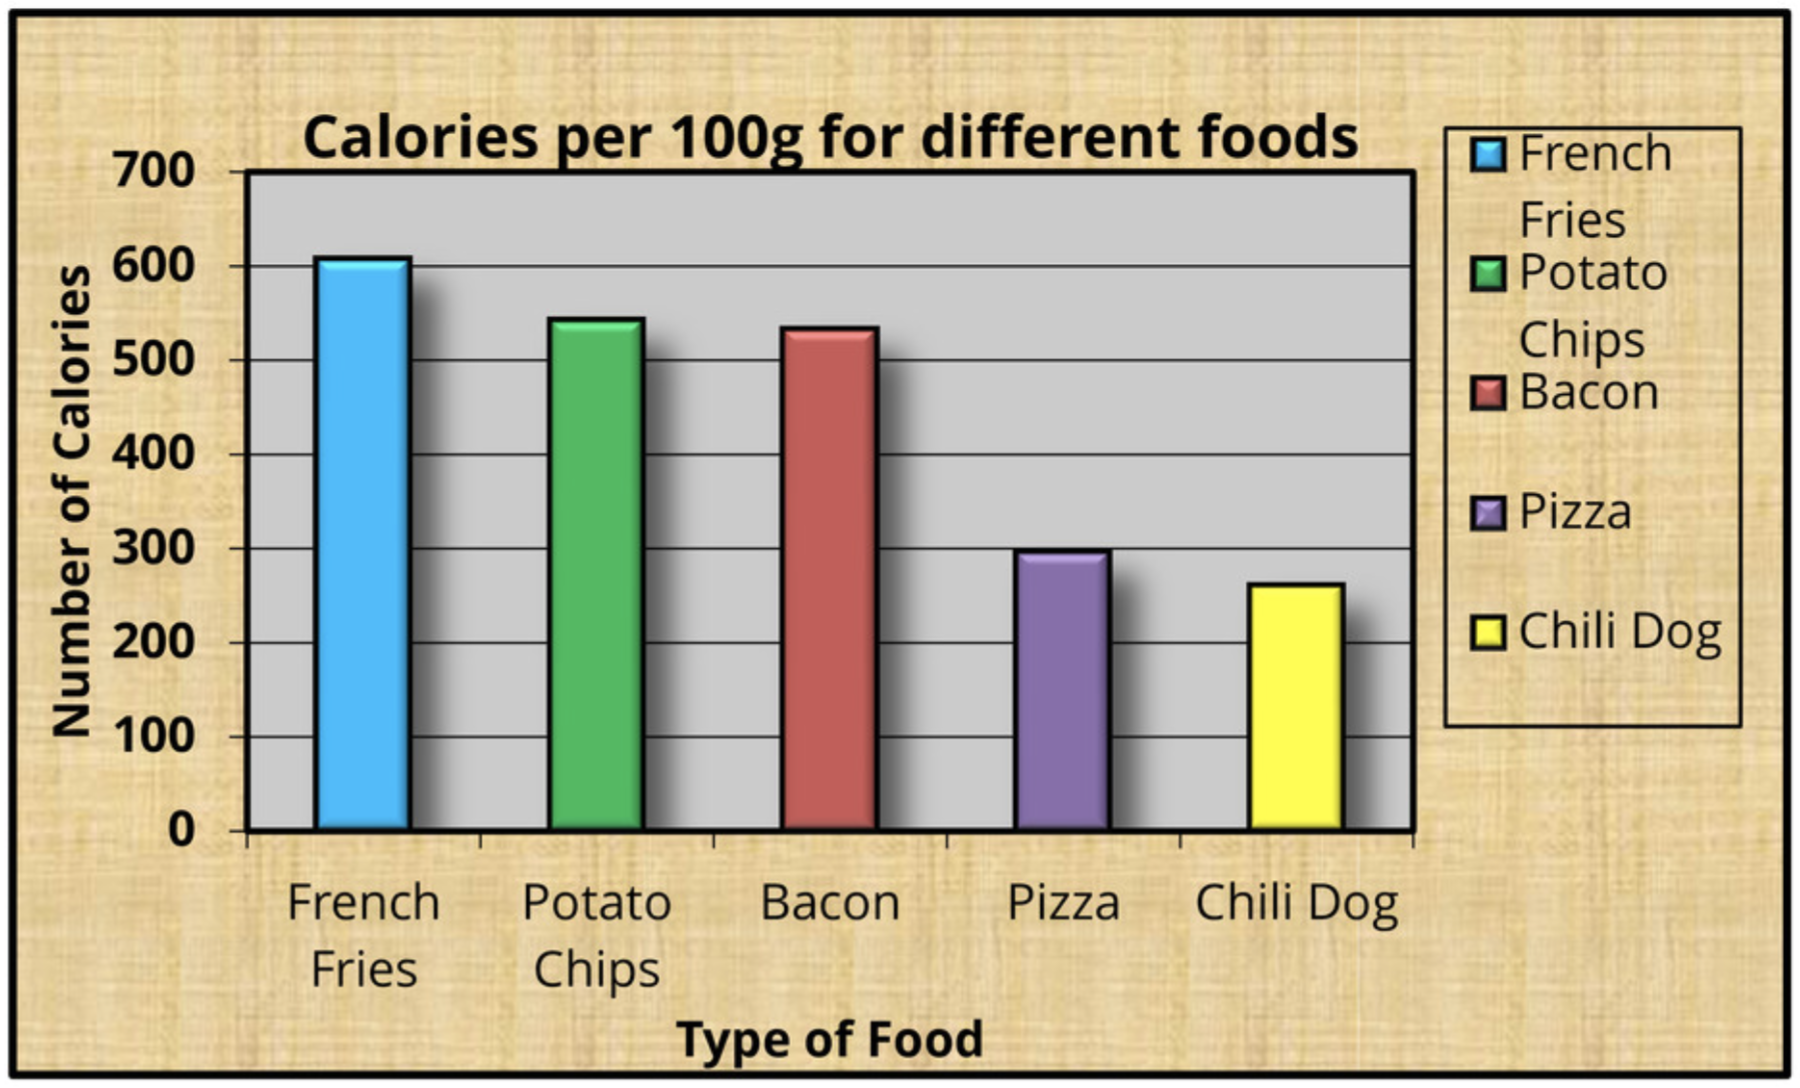
\includegraphics[width=\textwidth]{../figures/barplot-before}
% 	\caption{This is a fancy barplot.}
% 	\label{fig:barplot-before}
% \end{figure}

\newcommand{\image}[5][t]{
	\begin{figure}[#1]
		\centering
		\includegraphics[width=#2]{../figures/#3}
		\caption{#4}
		\label{fig:#5}
	\end{figure}
}

% Custom command to insert two images next to each other with a margin caption
% This command uses 6 required and one optional arguments/parameters with the following meaning:
%
% Optional:
% 1 - Position of the figure (the default position is 't' for top; if no argument is provided, 't' is used
%
% Required:
% 1 - Path to the frist image (inside the figures folder)
% 2 - Path to the second image (inside the figures folder)
% 3 - Caption of the image
% 4 - Label for the image (a universal fig: is prepended)
%
% Required --------------------------------------------------------------------------------------
% Optional -----------------|		  |			    |					|					    |
% 						    V		  V (1)		    V (2)				V (3)				    V (4)
% Example Usage: \twoimages[h]{barplot-before}{barplot-after}{This is a fancy barplot.}{barplot-sidebyside}
%
% The result will be the same as:
%
% \begin{figure}[h]
% 	\centering
% 	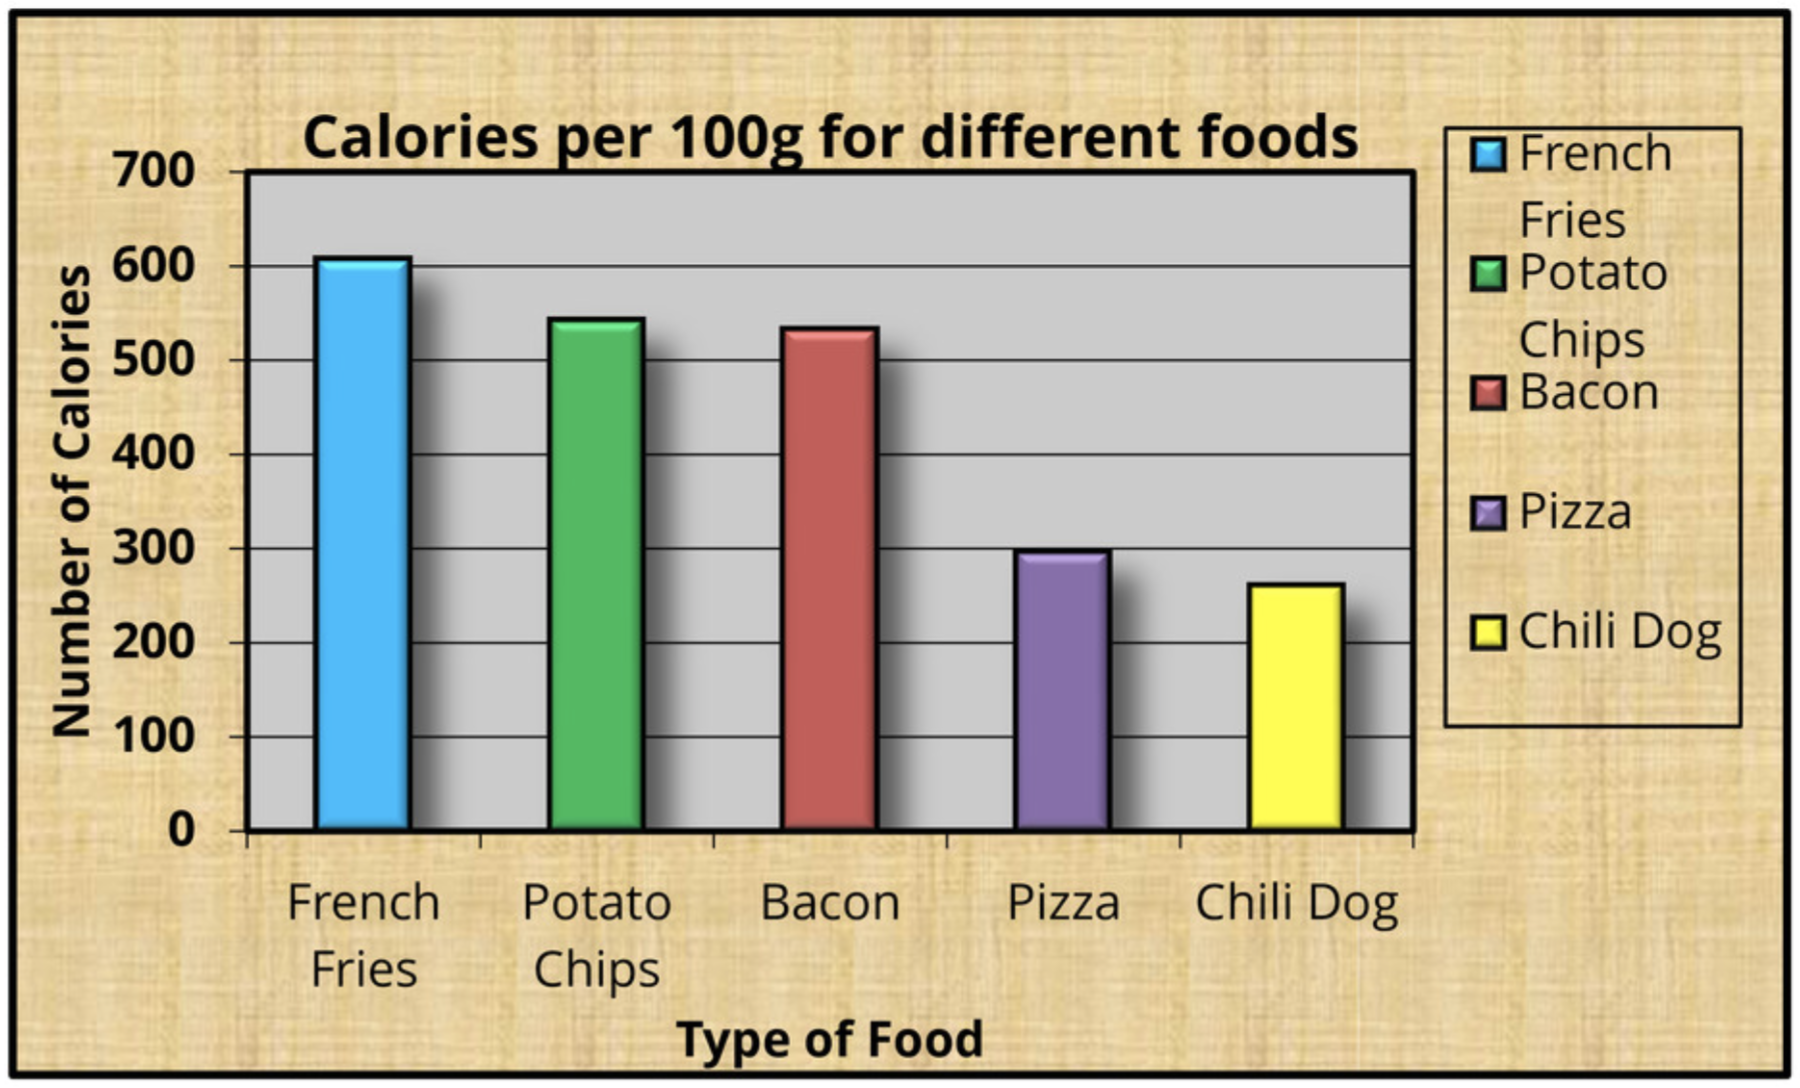
\includegraphics[width=0.48\textwidth]{../figures/barplot-before}
% 	\hspace{\fill}
% 	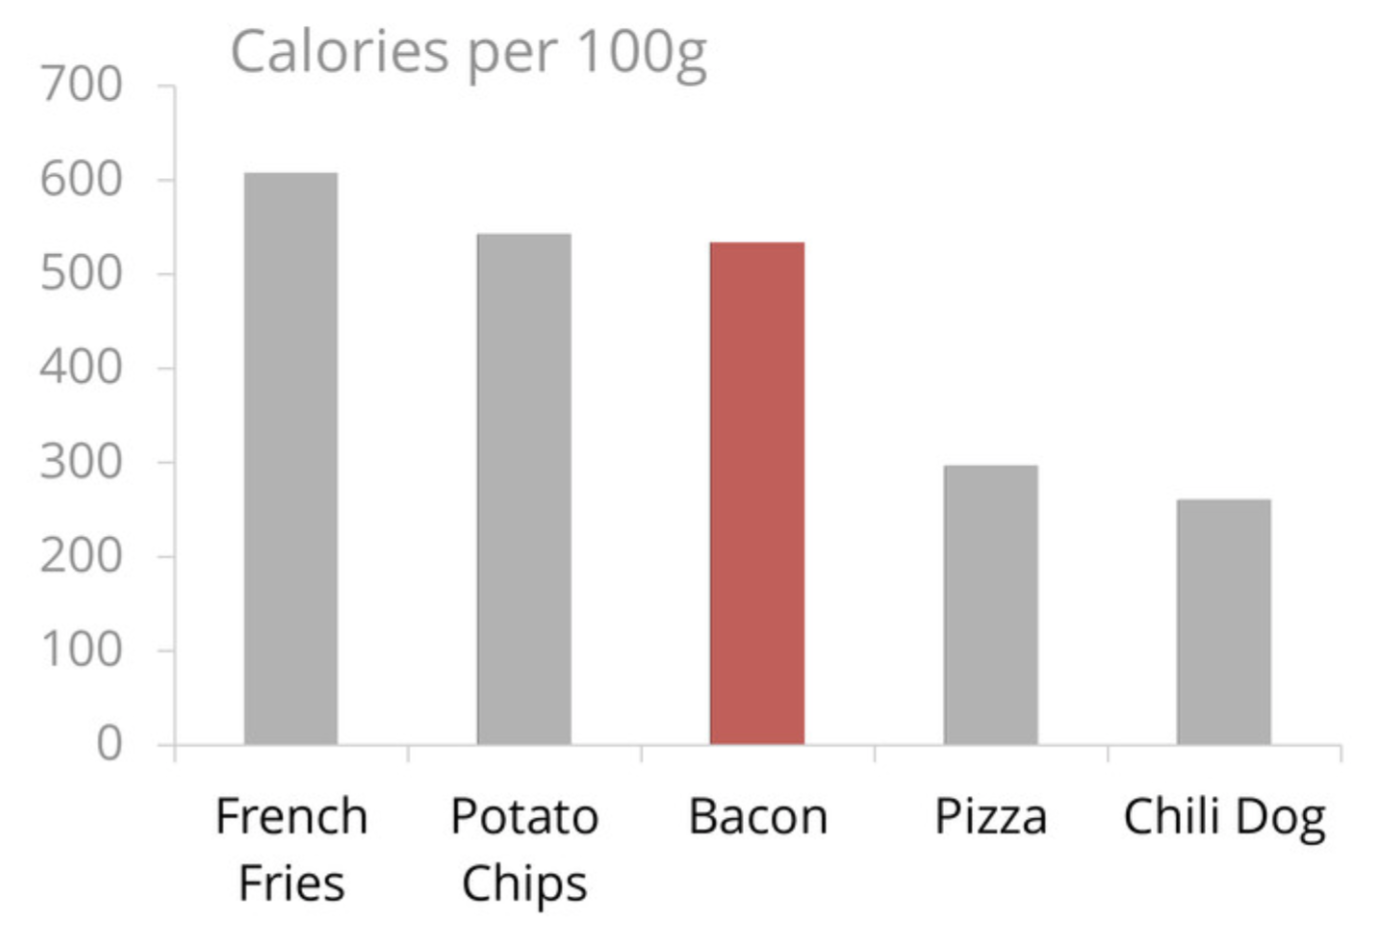
\includegraphics[width=0.48\textwidth]{../figures/barplot-after}
% 	\caption{\label{fig:barplot-sidebyside}This is a fancy barplot.}
% \end{figure}

\newcommand{\twoimages}[5][t]{
	\begin{figure}[#1]
		\centering
		\includegraphics[width=0.48\textwidth]{../figures/#2}
		\hspace{\fill}
		\includegraphics[width=0.48\textwidth]{../figures/#3}
		\sidecaption{\label{fig:#5}#4}[-2\baselineskip]
	\end{figure}
}


% Custom image command for wide figures
% This command uses 4 required and one optional arguments/parameters with the following meaning:
%
% Optional:
% 1 - Position of the figure (the default position is 't' for top; if no argument is provided, 't' is used
%
% Required:
% 1 - Path to the image (inside the figures folder)
% 2 - Caption of the image
% 3 - Label for the image (a universal fig: is prepended)
%
% Required ------------------------------------------------------------------
% Optional -----------------|		  |				 	 |					|
% 						    V		  V (1)		 	  	 V	(2)				V (3)
% Example Usage: \wideimage[h]{barplot-before}{This is a fancy barplot.}{barplot-before}
%
% The result will be the same as:
%
% \begin{figure*}[h]
% 	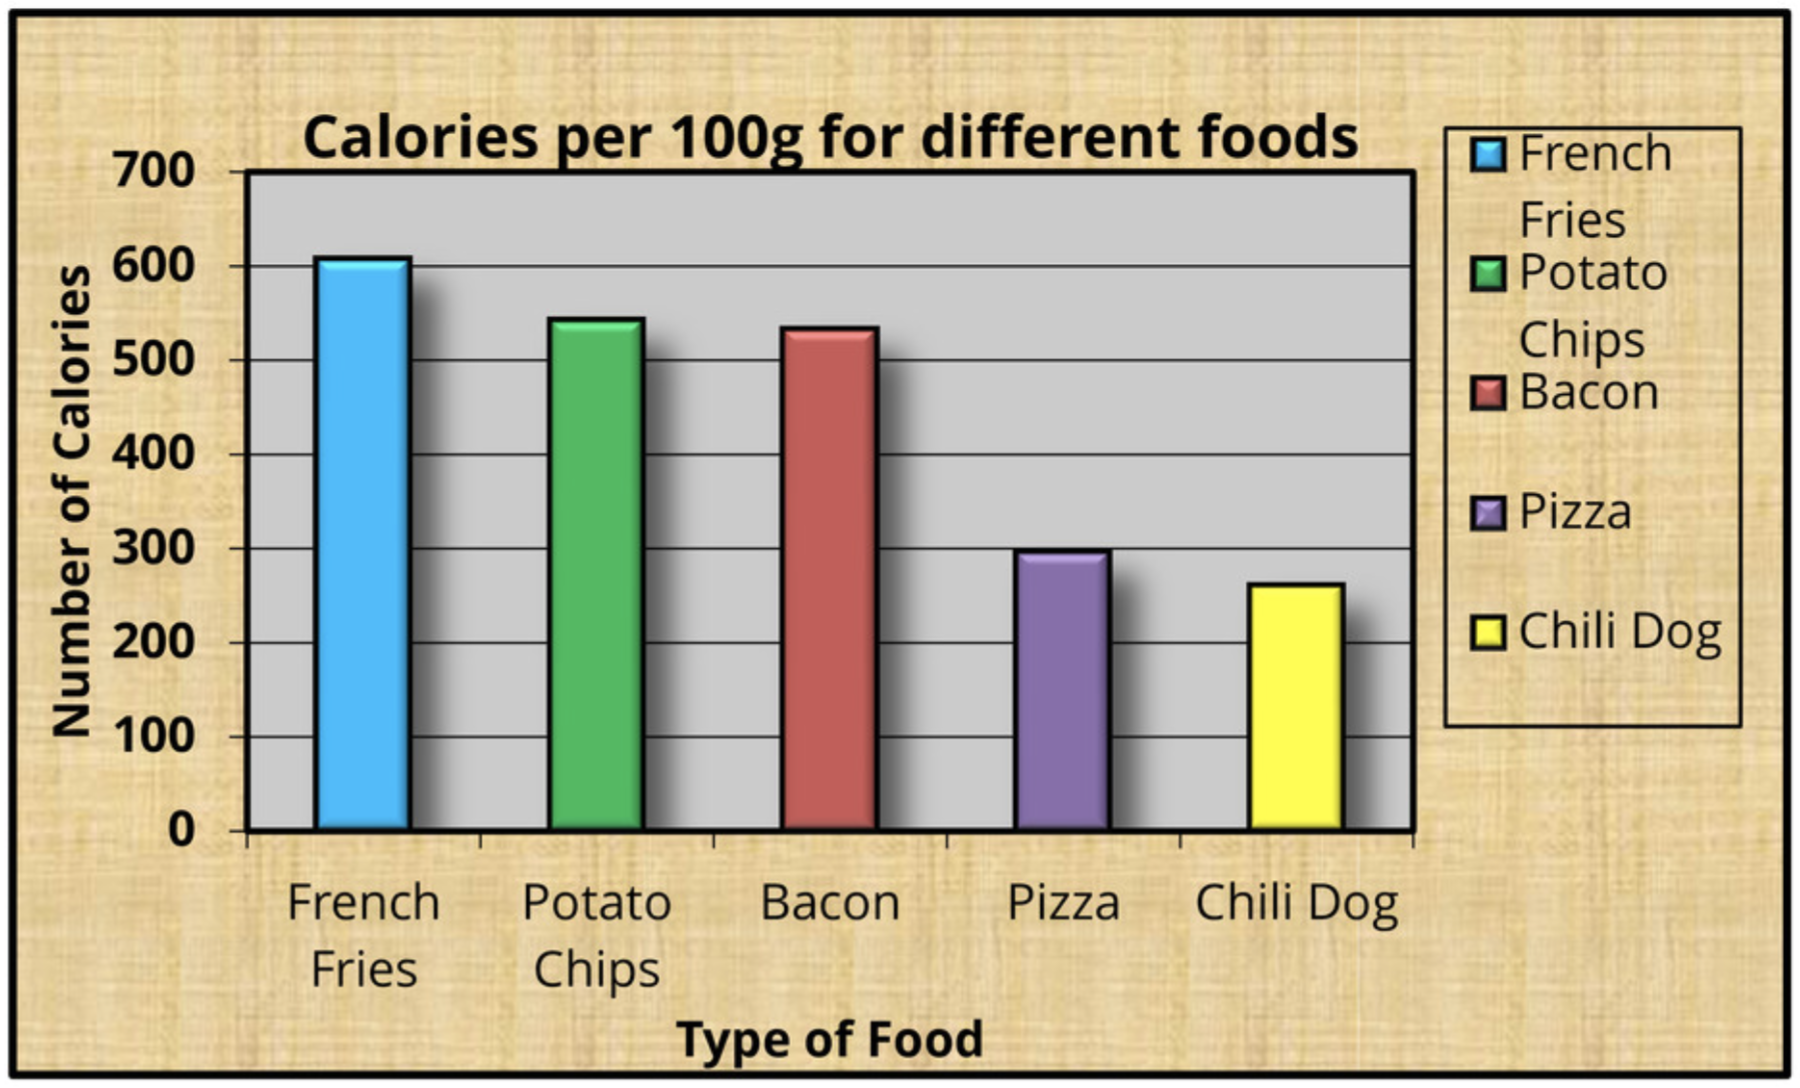
\includegraphics[width=\widefigurewidth]{../figures/barplot-before}
% 	\caption{This is a fancy barplot.}
% 	\label{fig:barplot-before}
% \end{figure*}
%
% %%%%%%%%%%%%%%%%%%%%%%%
% % 	ATTENTION		%
% %%%%%%%%%%%%%%%%%%%%%%%
% It seems this command messes with the position of other images, therefore it is advised to check the placement of other images.

\newcommand{\wideimage}[4][t]{
	\begin{figure*}[#1]
		\includegraphics[width=\widefigurewidth]{../figures/#2}
		\caption{\label{fig:#4}#3}
	\end{figure*}
}

% This command uses 3 required and one optional arguments/parameters with the following meaning:
%
% Optional:
% 1 - Vertical offset of the figure (the default offset is 1 for one line lower (negative numbers move the image up); if no argument is provided, 1 is used
%
% Required:
% 1 - Path to the image (inside the figures folder)
% 2 - Caption of the image
% 3 - Label for the image (a universal fig: is prepended)
%
% Required ----------------------------------------------------------------------
% Optional -------------------|			|				  |						|
% 							  V			V (1)			  V	(2)					V (3)
% Example Usage: \marginimage[2]{barplot-before}{This is a fancy barplot.}{barplot-before}
%
% The result will be the same as:
%
% \begin{marginfigure}[2\baselineskip]
% 	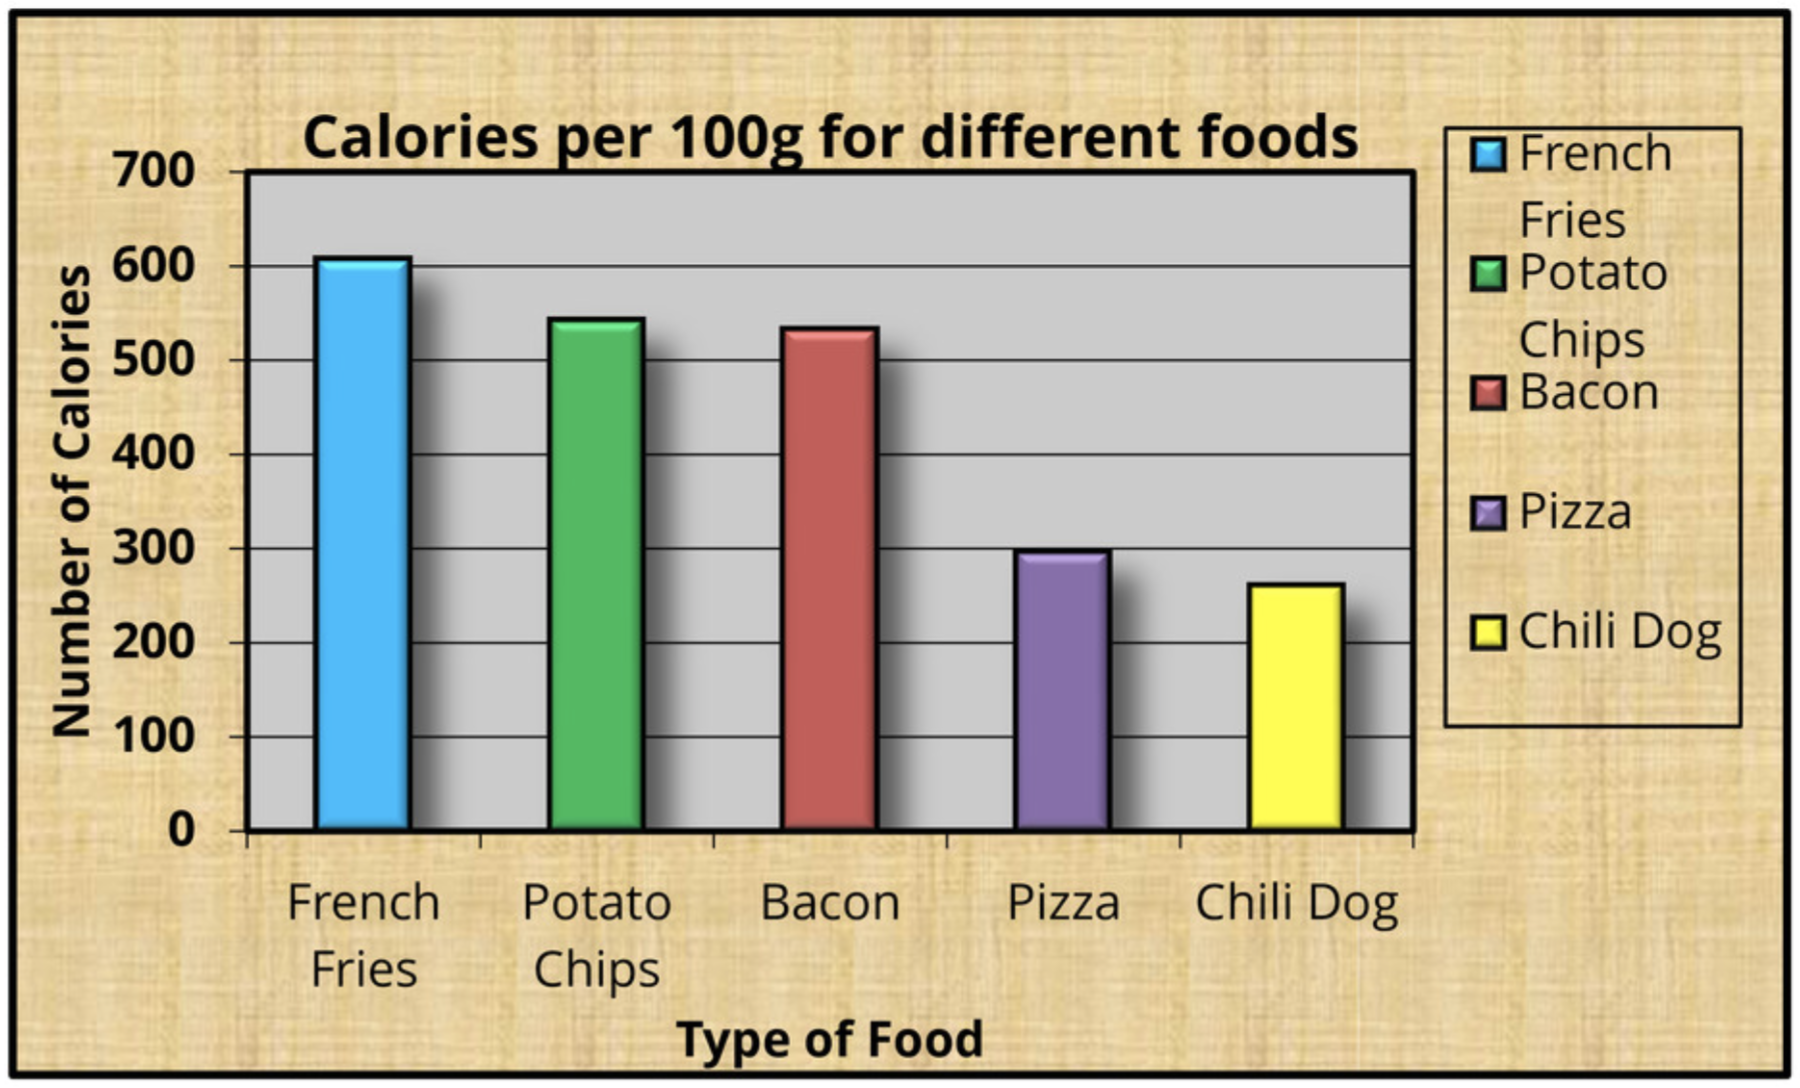
\includegraphics[width=\marginparwidth]{../figures/barplot-before}
% 	\caption{\label{fig:barplot-before}This is a fancy barplot.}
% \end{marginfigure}
\newcommand{\marginimage}[4][1]{
	\begin{marginfigure}[#1\baselineskip]
		\includegraphics[width=\marginparwidth]{../figures/#2}
		\caption{\label{fig:#4}#3}
	\end{marginfigure}
}
 % Load the custom commands from Misc/commands.tex

% Uncomment this command to make all links black:
%   useful for printing on black-white printers that do a
%   poor job at rasterizing colored text properly
%\hypersetup{colorlinks=false}

\addbibresource{literature.bib} % The filename of the bibliography

%----------------------------------------------------------------------------------------
%	THESIS INFORMATION
%----------------------------------------------------------------------------------------
\newcommand{\thesistype}{Master} % type of your thesis (Bachelors, Masters, Doctoral ...)

%%% CHANGE THIS:
% Your thesis title, this is used in the title and abstract, print it elsewhere with \ttitle
\thesistitle{Transformer-based Mobile Malware Detection}

% date to be printed on the title, this will automatically update and be in the correct format
% If any changes to this format (Month JJJJ) are necessary the definition can be found in line 337
% of misc/setup.tex
\def\tdate{\monthyeardate\today}

%%% CHANGE THIS:
% Your name, this is used in the title page, print it elsewhere with \authorname
\author{Joshua-Leon Dreger}

% Your supervisor's name, this is used in the title page, print it elsewhere with \supname
\supervisor{Prof. Dr. Konrad Rieck}

% Your university's name and URL, this is used in the title page, print it elsewhere with \univname
\university{\href{https://www.tu.berlin/en/}{Technische Universität Berlin}}

% Your research group's name and URL, this is used in the title page, print it elsewhere with \groupname
\group{\href{https://mlsec.org/index.html}{Machine Learning and Security (MLSEC)}}

% Your department's name and URL, this is used in the title page, print it elsewhere with \deptname
\department{\href{https://www.bifold.berlin/}{Berlin Institute for the Foundations of Learning and Data (BIFOLD)}}

% Your faculty's name and URL, this is used in the title page, print it elsewhere with \facname
% TODO: insert *your* degree program in the \faculty command below
% Applied Computer Science
% Computing in the Humanities
% Information Systems
% International Information Systems Management
% International Software Systems Science
% Software Systems Science
% Education in Business and Information Systems
\faculty{Information Systems Management Degree Program in the\\ \href{https://www.tu.berlin/en/eecs}{Faculty of Electrical Engineering and Computer Science}}

% Your address, this is not currently used anywhere in the template, print it elsewhere with \addressname
\addresses{address not used}

% Your subject area, this is not currently used anywhere in the template, print it elsewhere with \subjectname
\subject{subject not used}

% Keywords for your thesis, this is not currently used anywhere in the template, print it elsewhere with \keywordnames
\keywords{keywords not used}
%----------------------------------------------------------------------------------------
%	END OF THESIS INFORMATION
%----------------------------------------------------------------------------------------


\begin{document}

\selectlanguage{english}

\frenchspacing % do not add additional hspace after end of sentence full stop dot.

\frontmatter % Uses roman page numbering style (i, ii, iii, iv...) for the pre-content pages

\hypersetup{urlcolor=black}

%%%%%%%%%%%%%%%%%%%%%%%%%%%%%%%%%%%%%%%%%%%%%%%%%%%
%
% File: titlepage.tex
% 
% This file is part of the PSIThesis.cls
% LaTeX documentclass
% 
% The code in this file is made available
% under the following license:
%
% LPPL v1.3c (http://www.latex-project.org/lppl)
%
%%%%%%%%%%%%%%%%%%%%%%%%%%%%%%%%%%%%%%%%%%%%%%%%%%%


\pagestyle{plain} % Default to the plain heading style until the thesis style is called for the body content

%----------------------------------------------------------------------------------------
%	TITLE PAGE
%----------------------------------------------------------------------------------------

\begin{titlepage}

\newgeometry{
	inner=4cm, % Inner margin
	outer=4cm, % Outer margin
	marginparwidth=0cm,
	marginparsep=0mm,
	bindingoffset=.5cm, % Binding offset
	top=2.5cm, % Top margin
	bottom=2.5cm, % Bottom margin
	showframe % Uncomment to show how the type block is set on the page
}

\begin{center}

\vspace*{.06\textheight}

% The logo of University of Bamberg. Do not use the logo without permission.
% Using it on the title page of a thesis is acceptable.
% TODO Add your own logo here. Do yourself and your readers a favor and use
%      a vectorized logo (PDF) instead of a bitmap (PNG, JPEG)

\includegraphics[width=35mm]{misc/UB_Logo_20mm_CMYK.pdf}

\vspace*{.06\textheight}

{\LARGE \textls[130]{\MakeUppercase{\univname}}\par}\vspace{2\baselineskip} % University name

% TODO uncomment the next line when you write a thesis to display the supervisor
%{\large \facname}
% TODO comment out the next line when you write a thesis
{\large ~} % For use in the guide

\vspace{1.5cm}

% TODO uncomment the next line when you write a thesis to display the supervisor
%\textsc{\Large \thesistype 's~Thesis}\\[1cm] % For use in the thesis
% TODO comment out the next line when you write a thesis
\textsc{\Large ~}\\[1cm] % For use in the guide

%\HRule \\[0.4cm] % Horizontal line
%
{\huge \bfseries \ttitle\par}\vspace{1cm} % Thesis title

%\HRule \\[1.5cm] % Horizontal line


\textsc{\Large by}\\[1cm]

{\Large \authorname}

\vspace{1.5cm}

% TODO uncomment the next two lines when you write a thesis to display the supervisor
%\emph{Supervisor:} \\
%\supname\\[1cm]
%% 

\groupname%\\[2cm] % Research group name and department name

\vfill

{\large \tdate} % Date

% TODO remove the following lines when you write a thesis
\vspace{0.25ex}

{\small \tversion}

\vspace{0.25ex}

{\small Links to this document:}\\
{\small \url{\doiurl}} (initial version)\\
{\small \url{\githuburl} (most recent version)}
% Remove lines up to this line

\vfill
\end{center}

\restoregeometry

\end{titlepage}


 % Typeset the titlepage

\hypersetup{urlcolor=ubblue80}


%----------------------------------------------------------------------------------------
%	QUOTATION
%----------------------------------------------------------------------------------------

% \vspace*{0.2\textheight}

% \noindent\enquote{\itshape Thanks to my solid academic training, today I can write hundreds of words on virtually any topic without possessing a shred of information, which is how I got a good job in journalism.}\bigbreak

% \hfill Dave Barry


%----------------------------------------------------------------------------------------
%	ABSTRACT PAGE
%----------------------------------------------------------------------------------------

\begin{abstract}
%\addchaptertocentry{\abstractname}
% uncomment to add the abstract to the table of contents (not recommended)

For an overview of this document, see \Cref{Evaluation}.

Provide a Thesis Abstract here (length: less than one page).

For a start, you may want to consult the concise instructions for writing the Summary Paragraph in \emph{Nature}: \url{https://www.nature.com/documents/nature-summary-paragraph.pdf}. Moreover, consider Markus Kuhn's advice on differentiating abstract and introduction: \url{https://www.lightbluetouchpaper.org/2007/03/14/how-not-to-write-an-abstract/}.

A boilerplate scheme for an abstract is as follows: devote 25\,\% of the space on the purpose and importance of the research (introduction), 25\,\% of the space on what you did (methods), 35\,\% of the space on what you found (results), and 15\,\% of the space on the implications of the research (cf. \url{https://writingcenter.gmu.edu/guides/writing-an-abstract}).

More concrete advice for writing abstracts can be found on the website of the Writing Center of the University of North Carolina at Chapel Hill (\url{https://writingcenter.unc.edu/tips-and-tools/abstracts/}). Some useful phrases for abstracts can be found at \url{http://dissertation.laerd.com/useful-phrases-when-writing-a-dissertation-abstract.php}

Finally, you may also want to consider the excellent guide by Kent Beck on how to write good abstracts, which focuses on conference papers:
\url{https://plg.uwaterloo.ca/~migod/research/beckOOPSLA.html}.

\end{abstract}


%----------------------------------------------------------------------------------------
%	ACKNOWLEDGEMENTS
%----------------------------------------------------------------------------------------

%\begin{acknowledgements}
% %\addchaptertocentry{\acknowledgementname}
% Add the acknowledgements to the table of contents (not recommended)
%
%The acknowledgments and the people to thank go here.
%\end{acknowledgements}


%----------------------------------------------------------------------------------------
%	TABLE OF CONTENTS
%----------------------------------------------------------------------------------------

\cleardoublepage

% Table of Contents uses a wider layout than the main content
\newgeometry{
		head=13.6pt,
		top=27.4mm,
		bottom=27.4mm,
		inner=24.8mm,
		outer=24.8mm,
		marginparsep=0mm,
		marginparwidth=0mm,
}
{
\hypersetup{linkcolor=black}
\tableofcontents % Prints the ToC entries
}
\restoregeometry

%----------------------------------------------------------------------------------------
%	DEDICATION
%----------------------------------------------------------------------------------------

% \dedicatory{For/Dedicated to/To my\ldots}


%----------------------------------------------------------------------------------------
%	THESIS CONTENT - CHAPTERS
%----------------------------------------------------------------------------------------
\mainmatter % From here on, numeric (1,2,3...) page numbering
\pagestyle{thesis} % Return the page headers back to the "thesis" style

% Define some commands to keep the formatting separated from the content
\newcommand{\keyword}[1]{\textbf{#1}}
\newcommand{\tabhead}[1]{\textbf{#1}}
\newcommand{\code}[1]{\texttt{#1}}
\newcommand{\file}[1]{\texttt{#1}}
\newcommand{\option}[1]{\texttt{\itshape#1}}

% Figures will automatically be searched for in the Figures subdirectory
\graphicspath{{./figures/}{./examples/}}

%%% CHANGES NEEDED HERE
%
% Include the chapters of the thesis as separate files from the Chapters folder
% Uncomment the lines as you write the chapters
% Mind the \input instead of the \include here, that change is necessary for the appendix formatting
% Due to the \input command you also need to provide the .tex file ending

%\chapter{The PSIThesis Template} % Main chapter title

\label{Chapter1} % For referencing the chapter elsewhere, use \ref{Chapter1}


T his introductory chapter will give you an overview of the PSI Thesis template and its usage.
It also contains pointers to recommended reading for learning \LaTeX{}.

The remainder of this document presents conventions and recommendations that will help you create a coherent and visually appealing thesis. \Cref{Chapter2} explains the most critical aspects of scientific writing, including citations, URLs, tables, figures, typography, and layout.

Additional advice, which our students found useful in the past, follows in \Cref{appendixa}. Advice on designing compelling figures and tables follows in \Cref{appendixb}. Less-often needed details about the template, its history, and licensing details can be found in \Cref{appendixc}.

\section{A Quick Welcome}

Welcome to this LaTeX thesis template guide.%
\sidenote{It is based on the guide of the \emph{MastersDoctoralThesis} template. The original text has been revised and extended. \emph{MastersDoctoralThesis} is available at \url{https://www.latextemplates.com/template/masters-doctoral-thesis}.}
The PSIThesis template has been created mainly for students who want to submit a high-quality Bachelor's or Master's thesis to the \emph{Chair of Privacy and Security in Information Systems} at the University of Bamberg (\url{https://www.uni-bamberg.de/psi/}). The template can also be used for seminar reports and PhD dissertations.

The PSITemplate and this thesis guide reflect, at least to some degree, the personal taste of members of the chair.
We encourage our students to use the template without any changes.\sidenote{If you \emph{do} have a different opinion on a particular aspect of the template or the guide, we will be happy to hear you out.}

The template and the guide are available under an open license (cf. Sect.~\ref{sec:license}). If you want to use the template for a thesis submitted at a different department or organization, feel free to make changes at your discretion.\sidenote{Redistribution of this guide and the template is subject to the details outlined in Sect.~\ref{sec:license}.}

If you wish to contribute to the template or the guide, you may create an Issue or a Pull Request in the public GitHub repository at \url{\githuburl}.

\section{Learning LaTeX}

If you are new to LaTeX, we recommended to carry on reading this section.

If you are writing a thesis and its subject is technical, then creating it in LaTeX is highly recommended. LaTeX allows you to focus on the essential writing without having to worry over formatting or wasting time arguing with your word processor.

LaTeX can professionally typeset documents that run to hundreds or thousands of pages long. With simple mark-up commands, it automatically sets out the table of contents, margins, headers, and footers and keeps the formatting consistent and visually pleasing. One of its main strengths is the way it can easily typeset mathematics, even \emph{heavy} mathematics.

LaTeX is not a \textsc{wysiwyg} (What You See is What You Get) tool, unlike word processors such as Microsoft Word or Apple's Pages. Instead, a document written for LaTeX is a simple, plain text file that contains \emph{no formatting}.
LaTeX is a \enquote{mark-up} language (like HTML): You tell the LaTeX processor about the desired formatting in simple commands amongst the text. For instance, if you want to use \emph{italic text for emphasis}, you write the \verb|\emph{text}| command and put the text you want in italics in between the curly braces.

\subsection{Introduction to LaTeX}

If you are new to LaTeX, there is an excellent eBook, \enquote{The Not So Short Introduction to LaTeX} (aka ``lshort''), which is freely available online.\sidenote{\url{http://www.ctan.org/tex-archive/info/lshort/english/lshort.pdf}.}

To learn how LaTeX works, we recommend creating small test documents to reduce complexity. You can also learn from others by looking at other templates.

\paragraph{A Short Math Guide for LaTeX}

If you are writing a technical or mathematical thesis, you may want to read \enquote{A Short Math Guide for LaTeX}.\sidenote{Find it under the \enquote{Additional Documentation} section towards the bottom of the page at \url{http://www.ams.org/tex/amslatex.html}.}
LaTeX supports many mathematical symbols, and it would take a great effort to memorize the commands for all of them. Sunil Patel's website shows the most common ones.\sidenote{%
\url{http://www.sunilpatel.co.uk/latex-type/latex-math-symbols/}}
You can use Sunil's page as a reference or crib sheet. The symbols are rendered as large, high-quality images, so you can quickly find the LaTeX command for the symbol you need.

\subsection{LaTeX Distributions}

The LaTeX distribution is available for Windows, Linux, and macOS\@.
On Windows and Linux systems, the recommended distribution is \textsc{TeX Live} (\url{https://www.tug.org/texlive/}).
The package for macOS is called \textsc{MacTeX} (\url{http://www.tug.org/mactex/}), and it contains all the applications you need -- bundled together and pre-customized -- for a fully working LaTeX environment and workflow.
\textsc{MacTeX} includes a custom dedicated LaTeX editor called \textsc{TeXShop} for writing your `\file{.tex}' files and \textsc{BibDesk}, a program to manage your references and create your bibliography section.



\section{Required Software}
\label{sec:requirements}

To use the PSIThesis template, you need a working LaTeX installation with \textbf{LuaLaTeX}, \textbf{biblatex}, and \textbf{biber}.%
\sidenote{This guide is known to work fine on TeX Live Version 2019 (LuaLaTeX 1.10.0, biber 2.14) and 2020 (LuaHBTeX 1.12.0, biber 2.15).}
Usually, these tools are available in a typical LaTeX installation. We have tested the template with TeX Live 2019 and 2020. We recommend to perform a \textbf{full installation} to ensure that all required LaTeX packages are available right away.

\paragraph{Known Issues}

If you are using an outdated version of lualatex, compilation may fail with \textbf{error: (vf): invalid DVI command (1)}. This is a known bug\sidenote{\url{https://de.comp.text.tex.narkive.com/fC1xfeb2/lualtex-microtype-error-vf-invalid-dvi-command-1}} in old versions of lualatex that is triggered by the \texttt{microtype} package. In this case, we recommend upgrading to a current version of TeX Live.

Moreover, there is a known layout issue with old versions of the \texttt{caption} package. This issue causes the captions of margin figures and wide figures to be laid out incorrectly. Versions 3.4 and 3.5 of the caption package (released in 2019 and 2020, respectively) are known to work well. You can update your TeX Live installation by running \texttt{tlmgr}.

Use a current version of TeX Live that is available at \url{https://www.tug.org/texlive/}. As of 2020, the TeX Live version packaged by \textbf{Debian Linux} contains outdated versions of lualatex and the caption LaTeX package, which will likely result in incorrectly laid out documents. This is why it is \textbf{recommended to install LaTeX on Linux using the TeX Live installer}.

\paragraph{Using Overlaf and XeTeX}

As of December 2019, the template does not work with \url{https://www.overleaf.com}. Overleaf uses the outdated version lualatex~1.07 from TeX Live 2018, which is subject to the bug mentioned above that prevents compilation of documents that use the \code{microtype} package.

The template includes \code{microtype}, not only because of the better typography but also because it uses microtype's command \verb|\textls{text}| to change the letter spacing of the uppercase text on the title page.

You \emph{can} use the template with Overleaf if you remove the line that loads the \code{microtype} package in \file{setup.tex}. Moreover, you will have to remove all calls to \code{textls}.

Another option is typesetting the template with XeTeX. To compile the template with XeTeX, you have to remove the line that loads the package \code{luainputenc} from \file{setup.tex} as well as all calls to \code{textls}.


\section{Getting Started with the Template}

Once you are familiar with LaTeX, you should explore the directory structure of the template (cf. \Cref{sec:folders,sec:files}). Before you start to make changes, we recommend you to compile this guide on your machine (cf. \Cref{sec:compile}).
If there are no errors, it is time to place your details into the THESIS INFORMATION block of the \file{main.tex} file (cf. \Cref{sec:fillingdetails}).
You will also have to make some changes to the file \file{misc/titlepage.tex}, which sets up the title page.\marginnote{Additional features of the template are described in \Cref{ThesisFeatures}.}[-1\baselineskip]


\subsection{Folder Structure}
\label{sec:folders}

This template comes as a single ZIP file that expands out to several files and folders. The folder names are mostly self-explanatory:

\keyword{Appendices} -- this is the folder where you put the appendices. Each appendix should go into a separate \file{.tex} file. You have to include your appendix files in \file{main.tex}.

\keyword{Chapters} -- this is the folder where you put the thesis chapters. Each chapter should go into a separate \file{.tex} file that is included from \file{main.tex}.\sidenote{The structure of a thesis may look like this:
\begin{itemize}
\item Chap. 1: Introduction
\item Chap. 2: Background information
\item Chap. 3: Experimental setup
\item Chap. 4: Implementation considerations
\item Chap. 5: Presentation of results
\item Chap. 6: Discussion of results \& limitations
\item Chap. 7: Conclusion and future directions
\end{itemize}
This chapter layout is specialized for an experimental thesis; your thesis may be different.
}

\keyword{Examples} -- this folder contains a Python script to generate a figure used in this guide. You do not need that folder for your thesis.

\keyword{Figures} -- this folder contains all figures for the thesis. These are the final images that will go into the thesis document.

Two additional folders contain files that are internally used by the template. The folder \keyword{fonts} contains the TTF and OTF files of the template's fonts, the folder \keyword{misc} contains \file{setup.tex}, \file{titlepage.tex}, and the logo of University of Bamberg.

\subsection{Files}
\label{sec:files}

Most of the template's files are plain text, and you can see their contents in a text editor. Important files are:

\keyword{literature.bib} -- This is a BibTeX file that contains all the bibliographic information for literature that you cite in the thesis.
You can write it manually, but there are reference manager programs (such as JabRef or BibDesk on macOS) that will create and manage it for you. Bibliographies in LaTeX are a subject of their own, and you may need to read about BibTeX before starting with this.

\keyword{main.pdf} -- This is your typeset thesis created by LaTeX. It is part of the template's ZIP file. When you compile the template, you should get an identical version.

\keyword{main.tex} -- This is the file that you tell LaTeX to compile to produce \file{main.pdf}.
It contains the framework and constructs that tell LaTeX how to layout the thesis. It contains many comments that explain the purpose of each line of code. Fill in your details into the THESIS INFORMATION block.

\keyword{titlepage.tex} -- This file creates the title page. In its original form, several elements (e.\,g., displaying your supervisor) are commented out because \file{titlepage.tex} sets up the title page of this document (i.\,e., the PSIThesis Guide). Please check the content next to the TODO markers and remove the comments as instructed.

\keyword{PSIThesis.cls} -- This is the class file that tells LaTeX how to format the thesis. You should not have to make changes here.

\keyword{setup.tex} -- This file loads and sets up additional LaTeX packages.
It controls the layout of the thesis. If you want to change the layout, you should do that here.

During compilation, LuaLaTeX and biber will create additional auxiliary files such as as
\file{main.aux}, \file{main.bbl}, \file{main.aux}, \file{main.blg},
\file{main.lof}, \file{main.log}, \file{main.lot}, and \file{main.out}.
The auxiliary files can be ignored or deleted. They will be regenerated  as needed.


\subsection{Compiling the PDF}
\label{sec:compile}

You have to compile this template with \texttt{lualatex} (or XeTeX, cf. Sect.~\ref{sec:requirements}). Using \texttt{pdfLaTeX} is not possible, because the template uses TTF and OTF fonts.

On Windows, you can use the TeXworks application for compilation. To obtain the final PDF, you have to compile \file{main.tex} with \code{lualatex}, then run \code{biber}, and once more compile \file{main.tex} with \code{lualatex}.

On Linux and macOS, you can use the provided \keyword{Makefile}.\sidenote{Alternatively, you should be able to compile the thesis by running \code{latexmk -lualatex -pdf main.tex}. If you use an IDE that does not support \emph{latexmk}, you can still compile the document by manually executing \emph{lualatex}, then \emph{biber}, and \emph{lualatex} once again.}
Just navigate to the ``en'' directory and enter \code{make} in a terminal. Running \code{make} will automatically call the programs \code{lualatex} (which creates the PDF) and \code{biber} (which is used to compile the bibliography).

The \code{make} command keeps track of changes in your source files. If you add additional files that should be tracked for changes, you should edit the list of files at the top of the \file{Makefile}.
Otherwise, \code{make} may refuse to compile a new version because it believes that \file{main.pdf} is already up to date. In this case, a call to \code{make clean} will help: It removes all files generated during compilation. After that, a call to \code{make} will regenerate them, including \file{main.pdf}.


We haven't prepared the template to be used with the convenient LaTeX editor \textsc{LyX}.\sidenote{\url{https://www.lyx.org}} LyX hides the LaTeX code from authors and offers a user interface that resembles a word processor.
If LaTeX code puts you off, check out LyX and start writing there. Eventually, you can still export the LaTeX source code and copy and paste it into the PSIThesis template. Be sure to reserve some days to debug compatibility issues.

\subsection{Filling in Your Information in \emph{main.tex}}\label{sec:fillingdetails}

You will need to personalize the thesis template by filling in your details in \file{main.tex} with a text editor or your favorite LaTeX environment.

Open the file and scroll down to the third large block titled \emph{THESIS INFORMATION}. You will see entries for \emph{University Name}, \emph{Department Name}, etc. Fill out the information about yourself, your group, and institution.%
\sidenote{If you write a thesis at the PSI Chair at the University of Bamberg, you can keep the defaults.}
You can also insert web links; if you do, make sure you use the full URL, including the \code{http://} for this. If you don't want these to be linked, remove the \verb|\href{url}{name}| and only leave the name.

Next, open the file \file{misc/titlepage.tex}. Remove and add the comments as instructed by the \emph{TODO} notes.\marginnote{\textbf{Do not forget to edit \emph{titlepage.tex}!}}

When you have done this, save all changed files and recompile \code{main.tex}. All the information you filled in should now be in the PDF. You can now begin writing your thesis.

%----------------------------------------------------------------------------------------

\subsection{More Information on \emph{main.tex}}

The \file{main.tex} file sets up the structure of the thesis. There are plenty of comments that explain the purpose of the code.
Each major document element is divided into commented blocks with titles in all capitals. Initially, there seems to be a lot of LaTeX code. Most of that code takes care of the formatting of the thesis, so don't worry about it.

Begin by checking that your information on the title page is correct. For the thesis declaration, your institution may insist on something different than the text given. If this is the case, replace the text in the \emph{DECLARATION PAGE} block.

After that, you can insert a page with a quote (disabled by default).
Next up is the abstract page, which concisely summarizes your work.
After the abstract, you can insert an acknowledgments page (disabled by default).
You can use this space to thank your supporters.

The table of contents and the list of figures and tables are taken care of for you.%
\sidenote{If you write a thesis at the PSI chair, your thesis should \emph{only} contain a Table of Contents (i.\,e., neither a List of Figures nor a List of Tables). Therefore, all remaining lists are disabled by default. You must change \file{main.tex}, if you want to add these lists to your document.}
The next pages are optional: a list of abbreviations, a list of the physical constants and numbers, and a list of mathematical symbols.
The next optional page contains a one-line dedication.

After the definitions of the lists, there is a block that includes all the individual chapters. Each chapter should be saved in a separate file and put into the \emph{chapters} folder.
Uncomment the respective lines (delete the \code{\%} character) as you add chapters to your thesis. Similarly for the appendices, uncomment the respective lines as you need them. Appendices should be saved in the \emph{appendices} folder.

The next block sets up the bibliography. The template uses the bibliography style \emph{alpha}. The alpha style creates reference labels that contain the first letters or initials of authors and a two-digit number for the year, such as \cite{Hintz02}.


\section{Your Turn Now}

The easiest way to start your thesis is to replace text in the existing files. You might want to keep copies of the \file{.tex} to look up the source code as you move on.

We hope that this template helps you get up to speed. The tedious task of setting up the structure has been taken care of for you. It's now your job to create the content.

Good luck and happy writing!


\chapter{Introduction} % Main chapter title

\label{Introduction} % For referencing the chapter elsewhere, use \ref{Chapter1}


Here should be a text that states:

- Problem Statement

- Objective

- Research Contribution


\chapter{Related Work} % Main chapter title

\label{related_work} % For referencing the chapter elsewhere, use \ref{Chapter2}

\section{Transformer}
\label{sec:rel_transformer}

Transformer models have revolutionized how sequential data is processed in deep learning. 
Introduced by Vaswani et al. (2017) in the foundational paper “Attention Is All You Need” 
\cite{attention}
, the Transformer architecture relies entirely on attention mechanisms.
This was a paradigm shift from the previously prominent Recurrent Neuronal Network (RNN) \cite{rnn} 
or Convolutional Neuronal Network (CNN) \cite{cnn} approaches.
Transformer enables parallel processing of sequence elements and captures long range dependencies 
more effectively than RNN based approaches. 
At its core, a Transformer uses a mechanism called self-attention to weigh the importance of different 
tokens in a sequence relative to one another, 
allowing the model to focus on relevant context regardless of its positional distance. 
This ability to draw global dependencies between input and output makes Transformers powerful 
for tasks like machine translation, where the entire input sequence informs each output element. 

\begin{marginfigure}[] % move figure up by 1 line -5\baselineskip
    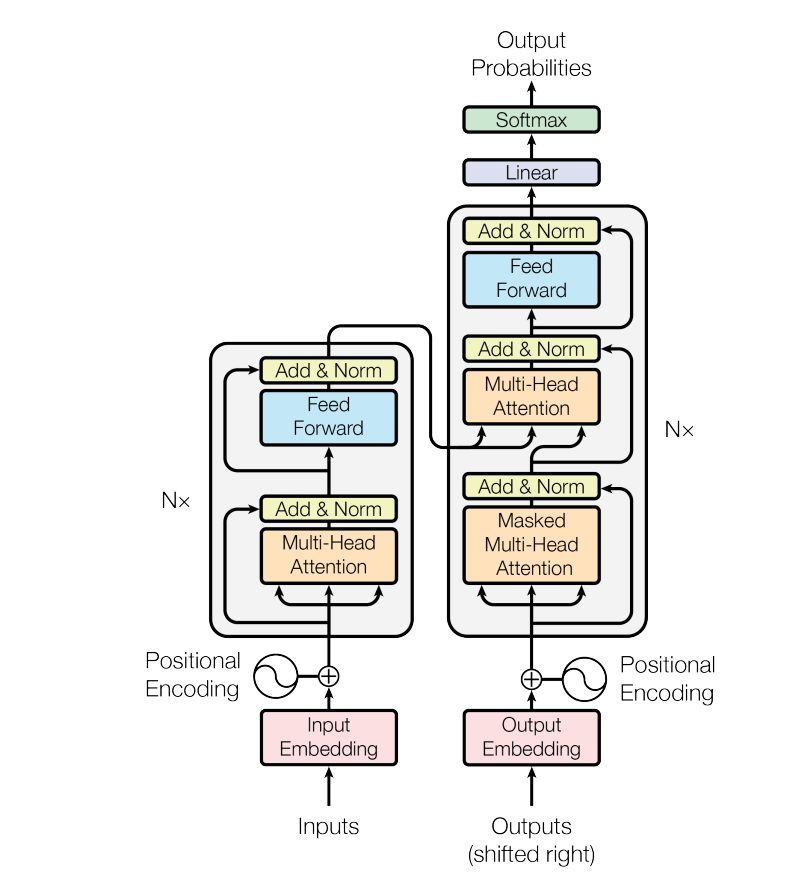
\includegraphics[width=1\marginparwidth]{2_RelatedWork/attention.png}
    \caption{\label{fig:malratios}
    Taken From \cite{attention}}
\end{marginfigure}

%Self-Attention
In a self-attention layer, the model computes attention scores between every pair of tokens in a sequence. 
Each token is first converted into an embedding vector, by looking up the token in the embedding matrix.
This embedding matrix has a row for each possible token in the vocabulary of the model.
Each row is the according embedding vector that represents this token. 
The embedding vector has a length of the "hidden size" hyperparameter of the model.
From each embedding vector then a Query (Q), Key (K), and Value (V) vector is derived.
This is done by multiplication of the embedding vector with
model specific learned projection matrices (One matrix for each Q, K \& V).
Next attention scores are obtained by multiplying Q and K vectors via a dot product. 
These scores determine how much attention one token should pay to another when constructing 
its next representation. 
After a softmax normalization layer, each token V vector aggregates information from all 
other tokens V vectors, weighted by these attention scores.
Finally, this weighted sum of V vectors produces a new contextualized embedding vector for that token, 
capturing relationships between words dynamically.
Transformers employ multi-head attention, meaning this process is replicated in parallel multiple times 
(with different learned projection matrices). 
Multi-head attention allows the model to attend to different patterns or aspects of the data simultaneously, 
capturing different kinds of relationships in the sequence. 
The outputs of multiple heads are then combined, 
enabling richer representations than a single attention operation. 
Because the Transformer has no recurrent notion of sequence order, 
it adds positional encodings to token embeddings to include information about each tokens position 
in the sequence.

%Encoder-Decoder
The original Transformer architecture is an encoder-decoder model, 
consisting of a stack of encoder layers and a stack of decoder layers
\cite{attention}. 
Each encoder layer has two main sublayers: 
a multi-head self-attention sublayer that allows each input token to attend to others, 
and a feed-forward network sublayer that further transforms each tokens embedding vector 
(each sub-layer is wrapped with residual connections and layer normalization for stability). 
Stacking multiple such layers produces an encoder that maps an input sequence into a sequence of 
high level feature vectors.
On the other side of the encoder-decoder, each decoder layer also contains 
a self-attention sublayer (applied to the decoders own inputs generated so far) and 
a feedforward sublayer, 
but additionally includes an encoder-decoder attention sublayer (also called cross-attention). 
This cross-attention allows the decoder to attend to the encoders output at each decoding step, 
effectively using the encoded source sequence context when predicting each token. 
The decoder generates one output token at a time, 
and each token embedding can only attend to earlier 
token embeddings (preventing a token from “seeing” future tokens during training). 
This encoder-decoder design proved extremely effective for sequence-to-sequence tasks like 
neural machine translation, 
where the encoder processes an input sentence into a context representation and 
the decoder generates an output sentence using that context \cite{deep_translate, gtrans}.


\begin{marginfigure}[] % move figure up by 1 line -5\baselineskip
    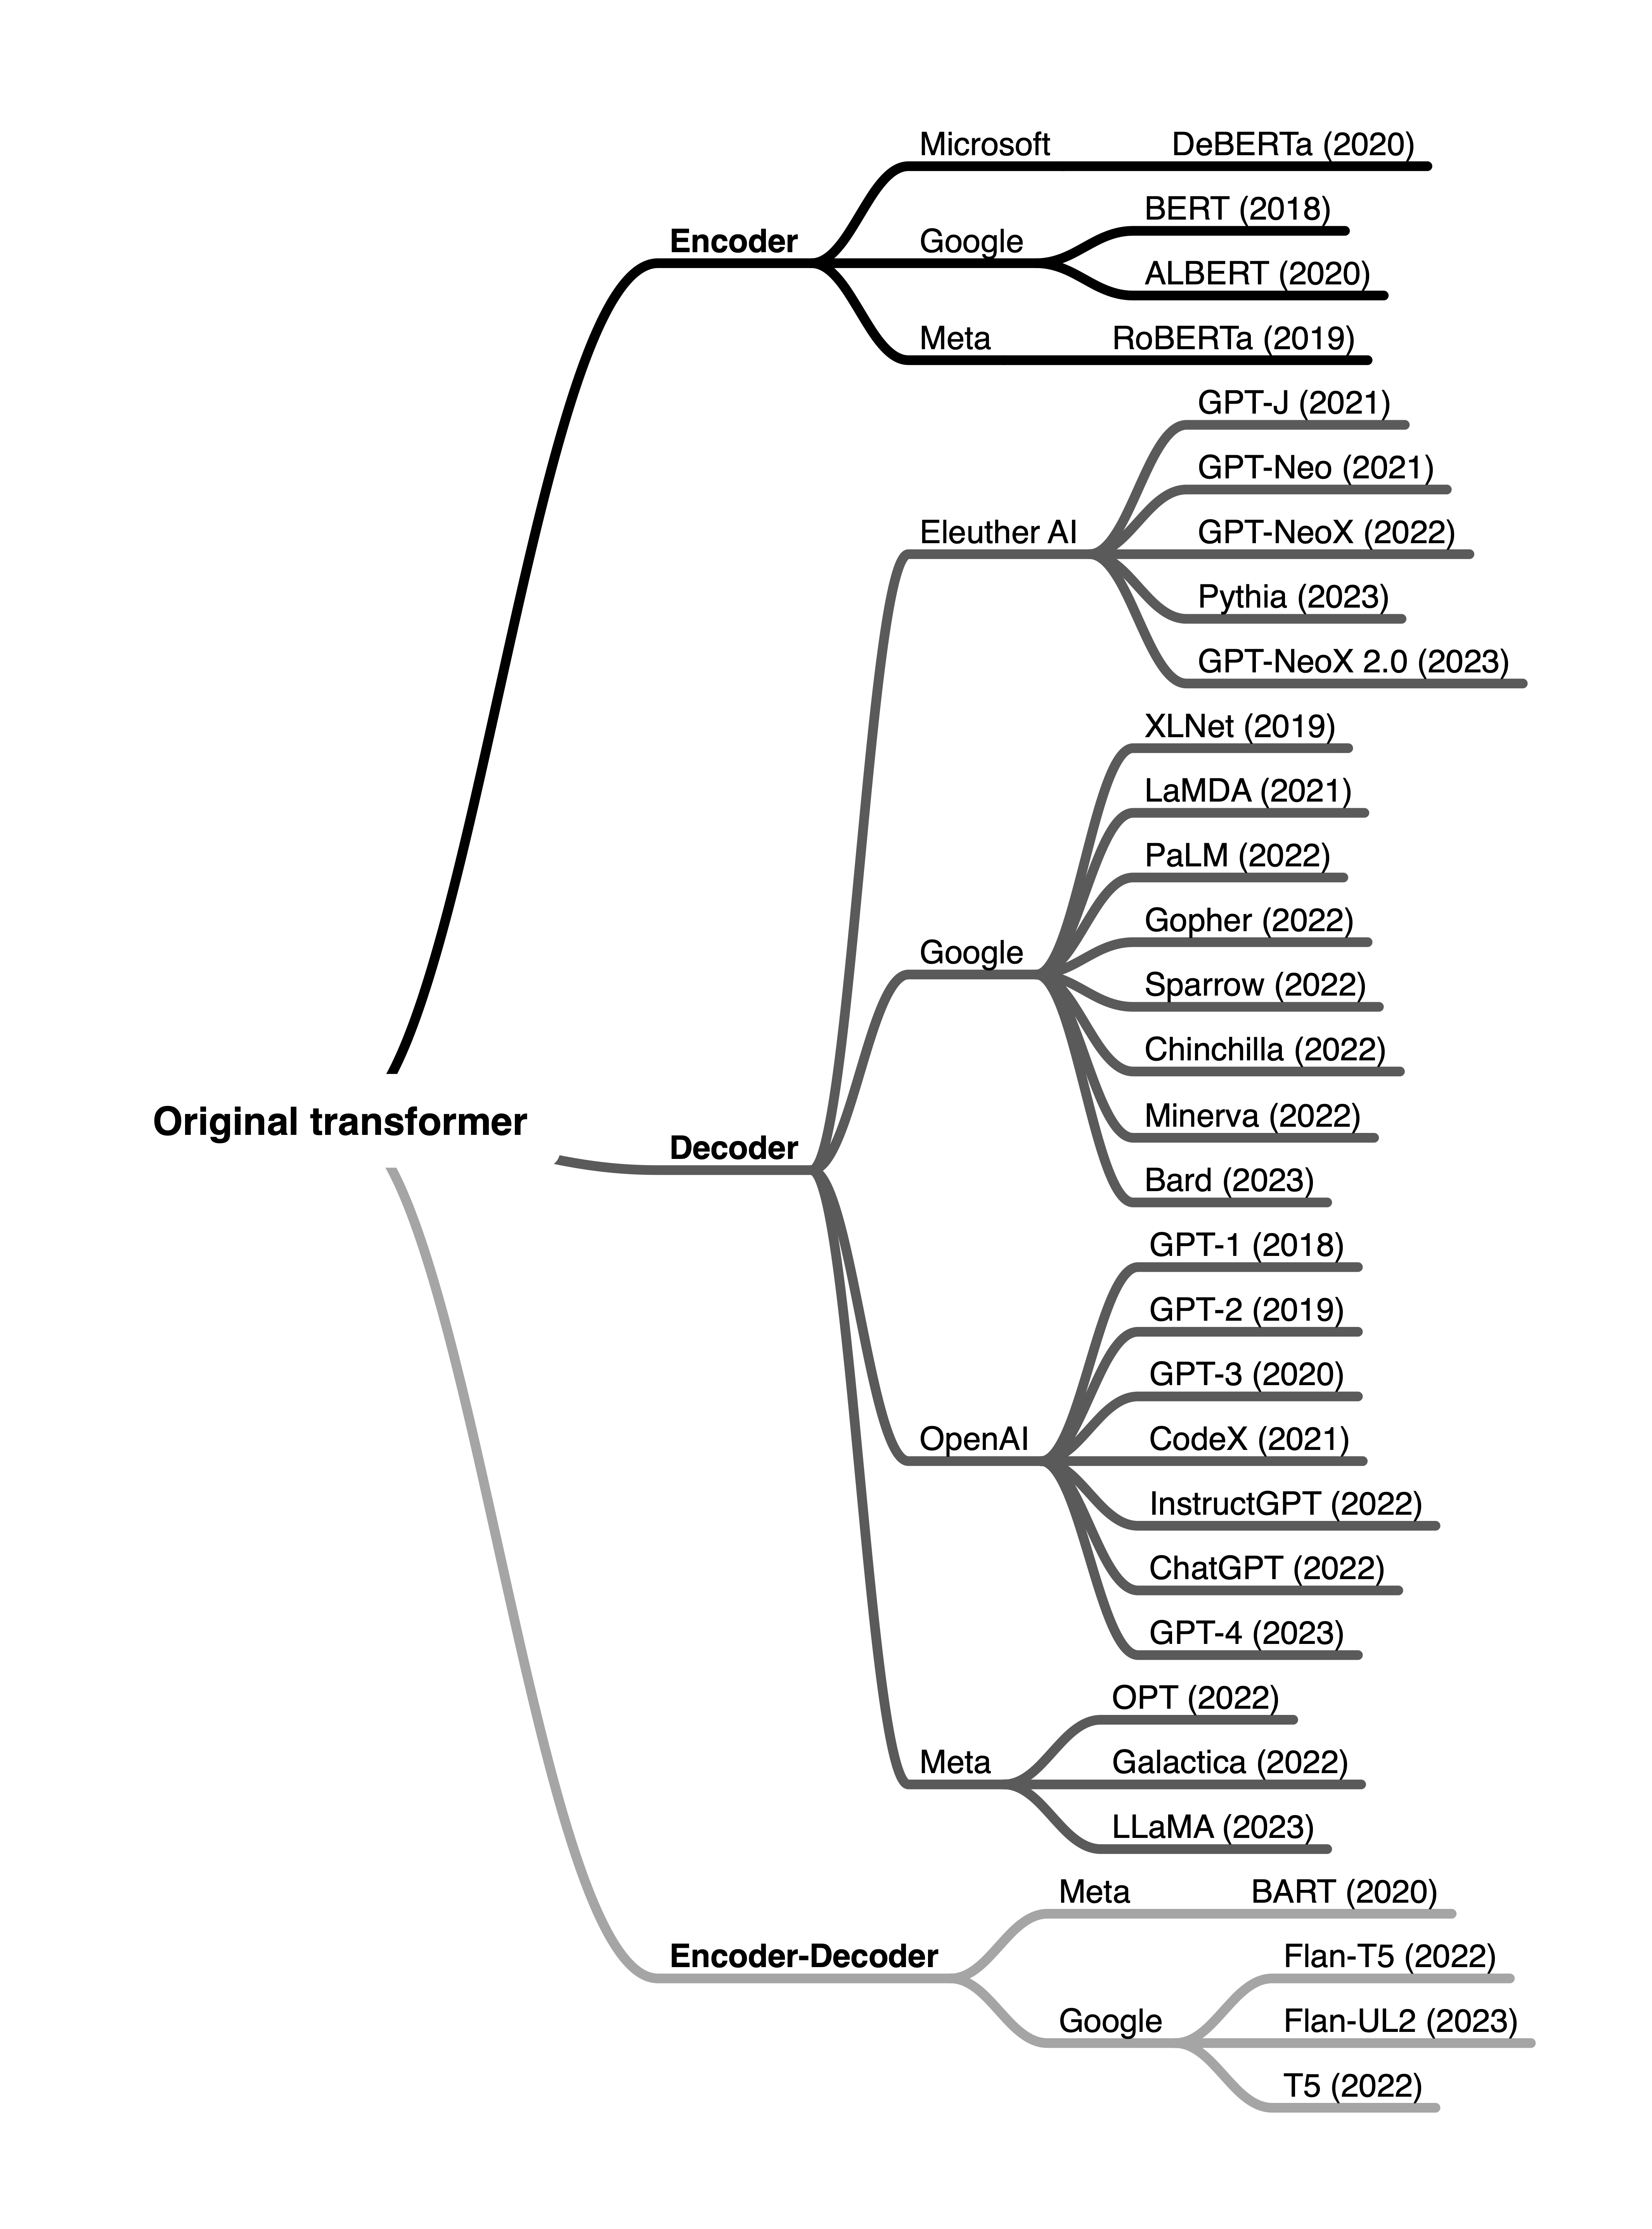
\includegraphics[width=1\marginparwidth]{2_RelatedWork/transformer_variants.png}
    \caption{\label{fig:malratios}
    Taken From https://magazine.sebastianraschka.com/p/understanding-encoder-and-decoder}
\end{marginfigure}

While the original Transformer uses both an encoder and a decoder, 
many modern applications use only one of the two stacks, depending on the task. 

%Encoder
Encoder only Transformer architectures
are designed exclusively with encoder components, 
leaving out the decoder segments present in encoder-decoder models. 
This design choice makes them particularly effective for tasks that require understanding and representation of input data 
without the necessity for sequence generation.
"Bidirectional Encoder Representations from Transformers" (BERT) \cite{bert} 
is a popular example
BERT is an encoder-only Transformer architecture that converts input text into a sequence of vectors representing the input text. 
It consists of multiple layers of encoders, each containing a self-attention mechanism and a feed-forward neural network. 
In BERTs pretraining, some tokens in the input are masked at random and the model must predict 
these missing tokens (Masked Language Modeling), 
and it also learns to predict if one sentence naturally follows another (Next Sentence Prediction). 
Through this process, BERT learns contextual embeddings that capture subtle relationships in language, 
as each tokens representation is influenced by the tokens on both its left and right. 
This bidirectional conditioning (as opposed to the one directional nature of a decoder) 
enabled BERT to achieve better performances on a wide range of NLP tasks once finetuned \cite{scoreBERT}.
In BERT's architecture, there is a special [CLS] token inserted at the beginning of each input sequence, 
serving as an empty sheet to be contextualized by the entire sequence for classification tasks. 
During training, the final hidden state corresponding to the [CLS] token is utilized to capture the overall meaning of the input.
The absence of a decoder in encoder only models means they are not typically used for generating new sequences from input data. 
Instead, they are used in scenarios where the goal is to derive meaningful representations or classifications from the input data.

%Decoder
Decoder-only Transformer architectures are built exclusively using decoder layers, 
leaving out encoder layers entirely. 
Such models are primarily designed for tasks that involve generating sequences, 
such as predicting text or continuing a given sequence. 
A prominent example is "Generative Pretrained Transformer" (GPT) \cite{gpt1, gpt2, gpt3, gpt4}, 
which is commonly used for text generation, summarization, and other creative writing tasks.
Each decoder layer includes two key parts: 
a self-attention mechanism and a feed-forward neural network. 
The self-attention allows the model to consider previously generated tokens when predicting the next one, 
helping it maintain context and coherence across a sequence. 
However, unlike encoder models, decoder-only models use a form of attention called "masked attention". 
This means each token can only pay attention to tokens that came before it, 
preventing the model from "seeing" future tokens during training or generation.
Decoder-only models like GPT learn by predicting the next token in a sequence, 
effectively teaching the model patterns in language and context over large datasets. 
Once trained, these models can generate coherent and contextually relevant sequences of text, 
making them powerful tools for tasks such as storytelling, dialogue systems, or code generation. 
Although decoder-only models excel at generating new text, 
they are usually less effective for tasks that require deep understanding or classification of input 
data compared to encoder or encoder-decoder models \cite{encoder_vs_decoder}.

Since "Attention Is All You Need", Transformer architectures have undergone numerous enhancements 
and there are a lot of different variants. 
Early on, researchers scaled Transformers to larger sizes and data 
(e.g., Llama 2 \cite{llama2}, Llama 3 \cite{llama3} for text generation) and created optimized versions of BERT 
(such as RoBERTa \cite{roberta}, ALBERT \cite{albert}, and DistilBERT \cite{distilbert}) 
to improve training effectiveness or model efficiency. 
A major focus has been on addressing the quadratic complexity of standard self-attention with respect 
to sequence length \cite{nystromformer}. 
Vanilla Transformers compute attention between all pairs of $n$ tokens, 
which scales with $O(n^2)$ in time and memory needed. 
This becomes a problem for long sequences like lengthy documents or code analysis 
(e.g., an entire mobile apps code can consist of thousands of tokens). 
Starting around 2020, new and more efficient Transformers emerged to tackle this limitation.

One notable example of an encoder only Transformer optimized for long text processing is Longformer \cite{longformer}. 
Longformer addresses the struggle of quadratic complexity by implementing a sparse attention pattern, 
allowing it to scale efficiently while preserving contextual understanding. 
Instead of each token attending to all others, Longformer uses a sliding window attention mechanism, 
where each token attends only to a fixed number of nearby tokens. 
Additionally, it employs global attention on select tokens (like the CLS token), 
enabling the model to capture broader contextual information across the sequence. 
This combination ensures efficient processing while keeping the ability to model long range dependencies. 
As a result, Longformer can process sequences of up to 4,000 tokens with a computational cost that grows linearly, 
rather than quadratically, with input sequence length. 
These design choices are supposed to make it  effective for tasks such as document classification, 
question answering, and summarization \cite{longformer}.

Another similar approach is BigBird \cite{bigbird}, 
which also uses sparse attention mechanism to efficiently handle long sequences while maintaining context. 
Like Longformer, BigBird reduces the quadratic complexity of traditional self-attention by limiting the number of attended tokens. 
However, BigBird extends the sparse attention paradigm by incorporating three types of attention: 
local attention, where each token attends to its nearest neighbors; 
random attention, where tokens attend to a few randomly selected tokens; 
and global attention (like the CLS token), where a small set of tokens attend to all others. 
This approach ensures that every token can at least indirectly attend to all others, 
maintaining the model's ability to capture long range dependencies.
BigBird can also process sequences up 4000 tokens, while maintaining linear complexity.
The authors claim that it is particularly suitable for long document NLP tasks such as 
question answering, summarization, and classification. 
Compared to Longformer, which primarily relies on windowed local attention and selected global tokens, 
BigBirds use of random attention supposedly allows for a better balance between efficiency and 
the ability to propagate information across distant tokens. 
Empirical studies have shown that BigBird outperforms Longformer in tasks requiring deep contextual understanding across long documents, 
such as multi-hop question answering and document classification \cite{bigbird}.

Another upgrade is promised by ModernBERT \cite{modernbert}.
ModernBERT is an optimized encoder only Transformer model that builds upon BERT while employing showing improvements in efficiency, 
scalability, and sequence length. 
Unlike the original BERT, which was limited to 512 tokens, ModernBERT extends its native sequence length to 8,192 tokens, 
making it more capable of handling long context tasks. 
This is achieved without introducing sparse attention mechanisms like Longformer or BigBird, 
instead using more efficient attention computation, better normalization techniques, and optimized training strategies.
A key feature of ModernBERT is its use of alternating attention layers, where some layers apply full global attention, 
while others apply localized attention to reduce computational overhead while maintaining strong contextual understanding. 
Additionally, Rotary Positional Embeddings replace BERTs absolute positional embeddings, 
allowing ModernBERT to generalize more effectively to long sequences. 
To further enhance efficiency, normalization is used before rather than after the attention sublayer, 
stabilizing training and improving gradient flow.
ModernBERT was trained on 2 trillion tokens, 
covering diverse domains such as long text documents, 
retrieval tasks, and code based datasets. 
Unlike previous BERT models, 
ModernBERT removes padding tokens during computation (a technique known as "unpadding"), 
reducing redundant operations and making inference more memory-efficient. 
These optimizations allow ModernBERT to match or surpass SOTA results across classification, retrieval, and multi-vector search tasks, 
while remaining faster and more scalable than its predecessors.
Compared to Longformer and BigBird, which rely on sparse attention mechanisms to scale to long sequences, 
ModernBERT maintains full bidirectional attention, ensuring stronger contextual modeling. 
While Longformer employs local windowed attention with select global tokens, and BigBird combines local, random, and global attention, 
ModernBERT balances efficiency end effectiveness through improved attention 
computation and optimized training techniques. 
This makes it a more general purpose solution, 
excelling in classification, retrieval, 
and document understanding, while remaining highly efficient for real world deployment on common GPUs \cite{modernbert}.

Another approach is Nyströmformer \cite{nystromformer} by Xiong et al. 
that applies the Nyström method (a technique for matrix approximation) to the self-attention computation.
Instead of computing the full $n \times n$ attention matrix, 
Nyströmformer samples a set tokens and uses them to construct an approximate attention matrix 
at only O(n) cost. 
This approximation allows the model to scale linearly with sequence length, 
a big improvement in efficiency. 
Nyströmformer reports competitive accuracy on many NLP tasks compared to 
standard Transformer, despite using only a fraction of the computation. 
This kind of efficient attention is especially relevant for resource constrained settings.
For instance, the recent DetectBERT \cite{detectbert} approach for Android malware analysis 
leveraged a Nyströmformer layer to handle a large amount of Embeddings at once 
(more details in section \ref{sec:detectbert}). 
By using Nyströmformer, DetectBERT reports to process each app in a single forward pass (up to ~8000 tokens) 
with only ~2 GB of GPU memory, achieving inference times on the order of 5 milliseconds per app. 

\section{Malware Detection}

Malware detection approaches are commonly categorized into static, dynamic, and hybrid analysis methods \cite{vorlesung}.
Each approach inspects malware from a different angle, 
offering unique advantages and tradeoffs in terms of accuracy, and efficiency.
While this thesis focuses on static analysis, it is worth noting the other approaches for context.
Static analysis examines APK features such as source code and binaries without executing the app.
The key advantage of static analysis is efficiency and scalability, 
since no runtime environment is needed, large volumes of files can be scanned quickly.
Prior research like \cite{drebin} and \cite{detectbert} demonstrate the effectiveness and efficiency of static approaches.
However, static analysis does face challenges, including evasion techniques.
Obfuscation and encryption can hide malicious code from static detectors.

Dynamic analysis, in contrast, executes the program in a controlled environment 
such as a sandbox\cite{sandbox}, to observe its behavior at runtime \cite{vorlesung}.
During execution, the analysis may monitor network traffic, file modifications, memory usage, 
and other behavior that may reveal malicious actions \cite{stateoftheartaibasedmalwaredetection}. 
A big advantage of dynamic analysis is that it can detect malicious behavior even if the code is obfuscated. 
This makes dynamic analysis more robust than static approaches.
Several research systems like TaintDroid \cite{taintdroid} or DroidScope \cite{droidscope} 
use this approach
However, dynamic analysis is computationally intensive and slower.
Running each APK in a virtual machine or virtual environment leads to a lot of computation, 
scaling this to thousands of files is very challenging.
Additionally, it is vulnerable to other evasive strategies, such as sandbox detection \cite{sandbox_detection}.

Hybrid techniques that integrate these methods aim to combine their strengths while weakening individual limitations.
Here both a parallel and integrated approach are possible.
In a parallel approach the malware set might first be clustered statically where the expensive dynamic approach then is only
applied to high risk malware. 
Alternatively also both static and dynamic features might be evaluated by the same model.
Hybrid analysis too, faces challenges such as computational and theoretical complexity.
This thesis, focuses on static analysis as a scalable and efficient approach for malware detection.

Malware authors often employ evasion techniques to bypass detection mechanisms \cite{vorlesung}.
In static analysis, common strategies include manipulating code structures through 
obfuscation \cite{obfuscation} and polymorphism \cite{polymorhism}.
Obfuscation involves transforming code into a more complex or less readable form to conceal its true purpose, 
whereas polymorphism allows malware to dynamically change its appearance while maintaining its core functionality.
These approaches exploit the limitations of analyzing code without running it.
While dynamic and hybrid methods address some of these weaknesses, 
they introduce their own vulnerabilities, such as susceptibility to sandbox detection and reliance on communication pattern anomalies.
Transformers ability to handle obfuscation and learn robust representations 
of static code helps mitigate some of these challenges \cite{deobfuscation}.
In addition to Transformers having the potential to be robust to obfuscation, they also show capabilities of deobfuscating code through 
encoder decoder systems as discussed in chapter \ref{sec:rel_transformer}.

Another challenge in the realm of malware detection is concept drift due to malware authors continuously evolving their techniques.
Concept drift refers to the evolution of malware patterns, which often leads to a decline in the performance of detection models over time.
Work like Transcend \cite{transcend} have tackled this issue by introducing mechanisms to detect and adapt to concept drift during deployment.
However, these methods are resource intensive and may struggle to generalize across diverse datasets.
Based on the Transcend approach the same research group published work on "Transcending Transcend" \cite{transcending}, where they used their 
mechanism to construct a dataset.
Addressing concept drift remains a critical challenge for static Android malware detection and is one criteria used in this thesis.
Some works have proposed automated drift detectors that trigger model updates when the 
input data distribution shifts \cite{morph}.

Somewhat similar to the challenge of concept drift is the challenge of biased datasets.
Tesseract \cite{tesseract} shows, how datasets are always biased and never represent the true distribution of software.
The authors differentiated bias in spatial and temporal bias.
The spatial bias stems from unrealistic class distributions,
such as an artificially high proportion of malware, which do not match real world conditions.
Temporal bias bases on concept drift and 
occurs when the data is trained and evaluated on the same timespan.
In real world scenarios malware detectors will always be trained until a certain point in time and will then be used to 
process new software. This means that a model has to be somewhat robust to concept drift. 
To account for temporal bias the authors propose to split the dataset that is used in a temporal manner, 
where the training data is comes before the evaluation data.
While still being biased, this time based split makes the evaluation of models more realistic.


\subsection{Android Malware Detection}
\label{sec:amd}

Detecting malware on the Android platform presents unique challenges and opportunities due to its open ecosystem 
and the high volume of apps and malware samples. 
The availability of many labeled datasets such as Androzoo, Drebin, Transcend, and DexRay has driven research in this domain.

Drebin \cite{drebin} is a static analysis method for detecting Android malware using machine learning. 
It extracts features from an apps manifest and code to build a set of descriptive strings. 
These features are encoded in a high dimensional vector space, where each APK is represented by a sparse binary vector. 
Drebin uses a linear Support Vector Machine (SVM) to learn a decision boundary that separates benign apps from malware. 
The method detects about 94\% of malware samples while keeping the false positive rate around 1\%. 
It is designed to be lightweight and can run directly on smartphones, typically taking about 10 seconds per application. 
The approach also provides explanations by showing the most important features that led to the detection. 
This helps users understand why an app is flagged as malicious. 
In addition, the Drebin dataset, which includes labeled malware samples and complete APK files, is a foundational 
resource for further research. 

Transcending \cite{transcending} introduces a dataset that spans five years of real-world Android applications. 
The dataset includes thousands of malware samples collected from sources like AndroZoo. 
It is split into training and testing sets that represent different time periods based on the work of Tesseract \cite{tesseract}.
The study showed that static detection models like Drebin trained on older data lose accuracy as new malware emerges. 
Based on the work of Transcend \cite{transcend} it introduces a rejection mechanism to identify samples that do not match the training distribution. 
This approach helps prevent misclassification by flagging drifting samples. 
By using this comprehensive dataset, the work highlights the impact of concept drift on static malware detection. 
It has set a new benchmark for evaluating the robustness of detection models over extended periods.
In this thesis we will call the dataset that was used in the Transcending paper Transcend.

DexRay \cite{dexray} is a deep learning approach that detects Android malware by converting app bytecode into a grey-scale vector image. 
It first extracts the raw DEX bytecode from an APK file and then transforms the bytes into a one dimensional image. 
This image is resized to a fixed size and fed into a simple one dimensional convolutional neural network for classification. 
The model is evaluated on a dataset of 158,803 Android applications collected from AndroZoo. 
The dataset spans apps from 2019 to 2020 and includes both benign and malicious samples. 
Benign apps are defined as those not flagged by any antivirus on VirusTotal \footnote{https://www.virustotal.com/gui/home/upload}, 
while malware apps are identified if at least two antivirus engines detect them. 
A key feature of the DexRay dataset is, that it includes both non obfuscated and obfuscated APKs. 
This design is supposed to allow researchers to study the impact of code obfuscation on detection performance. 
DexRay achieves an impressive F1-score of 96\%, demonstrating its effectiveness in malware detection. 
Its simple yet effective approach makes it a solid baseline for malware detection.

Androzoo \cite{androzoo} is a large repository that contains millions of Android apps collected from various app stores. 
It spans more than a decade of Android development, which makes it a valuable resource for studying long term trends. 
It includes both benign and malicious APKs, in addition to metadata for each app, such as compilation dates, sizes, antivirus reports and more. 
This extra information enables further analysis of the Android app landscape.
The scale and diversity of Androzoo have helped improve the reproducibility of research studies. 
Researchers can use Androzoo to track how malware evolves over time and to test the effectiveness of detection methods.
Androzoo enabled the research of this thesis by providing an API key to download APKs from its repository.
This key was then used to download the DexRay dataset to analyze it together with the previously mentioned ones in chapter \ref{sec:datasets}.

\section{Transformer based malware detection}

Recent research in cybersecurity has produced a range of Transformer based models for malware detection.
Many of these novel approaches build on the BERT 
\cite{bert} 
architecture or its variants, 
adapting them to capture the semantics of malicious code and improve detection performance. 
For example, MalBERT 
\cite{malbert}
uses a BERT variant that is finetuned on Android app manifest files for static analysis. 
By treating an apps manifest (which lists permissions, components, etc.) as input text, 
MalBERT achieved excellent results, with about 97\% accuracy and an F1 score around 95\% 
in distinguishing malware from benign apps, even when reproduced by other authors 
\cite{malbert_reproduce}. 
Its success indicates that Transformers can leverage even simple limited textual features (like manifests) 
for malware detection. 
However, focusing only on manifest content may miss code level clues e.g. 
obfuscated or malicious code could be overlooked if not reflected in the manifest. 
To address this, a followup model MalBERTv2 
\cite{malbert_two} 
extended the approach to be code-aware. 
MalBERTv2 processes actual app code by extracting the most informative code files and applying a 
custom tokenization before using a BERT based model.
This richer static analysis led to improved performance across multiple datasets: 
MalBERTv2 reports an F1 score of 97\% when evaluated on a mix of Android malware datasets.
On smaller subsets, MalBERTv2s F1 score ranged from about 82\% up to 94\%. 
These BERT based detectors demonstrate the Transformers ability to learn meaningful features from 
app data (manifest or code), resulting in high precision and recall. 
A limitation is that their large size (e.g. BERT base with 110 million parameters) can be expensive to train and execute. 

Purely codebased is another approach called DetectBERT \cite{detectbert}.
DetectBERT is a transformer based approach to Android malware detection that 
builds upon DexBERT \cite{dexbert}, 
another transformer based model designed for Smali class level analysis of Android Smali code.
Using a Correlated Multiple Instance Learning (c-MIL) framework, 
DetectBERT aggregates Smali class embeddings of DexBERT into an app level representation.
The DetectBERT model is further analyzed in Chapter \ref{sec:detectbert} where it is evaluated as baseline.

Another recent model, BERTroid 
\cite{bertroid}
, further showcases Transformers potenital in Android malware detection. 
BERTroid is based on a BERT architecture and integrates neural embeddings from both static and dynamic 
analysis to classify apps. 
It was evaluated on several public datasets. 
BERTroid is reports to outperform prior SOTA solutions, achieving near perfect detection rates 
for instance, an Accuracy of 99.74\% and F1-score of 99.87\% on one benchmark, 
with precision and recall also around 99.87\%. 
Such results indicate a very high true positive and true negative rate. 
The authors note BERTroids resilience against concept drift, 
claiming it maintains high performance even as malware characteristics change over time. 
This hints that training on diverse and up to date data empowered the model to be robust to concept drift. 
It should be noted, however, that achieving nearly 99\%+ 
accuracy in malware detection can sometimes be a sign of evaluation on simplified scenarios 
real world deployment may see lower numbers due to novel malware samples or adaptive attackers. 
Nonetheless, BERTroid underscores the effectiveness of Transformer encoders in this domain. 

Similarly, Liu et al. propose SeMalBERT 
\cite{semalbert}
, which focuses on learning semantic representations of code using BERT. 
SeMalBERT achieved high detection rates, with accuracy improving from about 88.6\% up to ~98.75\%. 
This suggests that capturing semantic meaning makes the detector more robust to code obfuscation 
and variants, since semantically similar malware will be clustered in the Transformers feature space 
even if their surface syntax differs. 
Roziere et al. showed that pretrained Transformers can deobfuscate code and 
recover its functionality to an extent 
\cite{deobfuscation}
, underscoring the potential for resilience against obscured or polymorphic code. 
One key advantage is their ability to learn deep, contextual representations of code and API usage, 
which helps in resisting many common obfuscation techniques. 
Traditional static detectors often rely on specific keywords, signatures, or simple features that 
malware authors can easily obfuscate (e.g., renaming variables, reordering code, ...).
Transformers, by contrast, attend to the broader context and meaning of code tokens.
That said, Transformers are not impervious to obfuscation, especially sophisticated obfuscation that 
changes control flow or encrypts malicious payloads. 
In such cases, the model might not see any learned pattern unless it has been trained on 
similarly obfuscated examples. 

Another strength of Transformers is their capacity to incorporate multiple feature types. 
As seen, some models combine textual code features with other modalities (images, graphs, etc.), 
and the attention mechanism can naturally combine information from different sources. 
This is valuable in malware detection, where one may want to consider app permissions, 
API calls and graphs together. 
The HTGT (Heterogeneous Temporal Graph Transformer) 
\cite{htgt}
is a prime example: 
it jointly models an entire Android malware ecosystem as a graph with various entity types 
(apps, developers, markets) and learns relations both spatially (graph connections) and temporally 
(evolution over time). 
By using a specialized Transformer on this heterogeneous graph, 
their system (called Dr.Droid) can detect malware while explicitly tracking how malware 
evolves. 
This approach directly tackles concept drift: as new malware appears, 
the temporal graph Transformer updates the representation of the “drifting” nodes, 
helping to catch novel threats that differ from past training data. 
In evaluations on large scale industry data from Tencent Security, 
HTGT significantly outperformed baseline detectors on identifying evolving Android malware, 
and notably Dr.Droid has been deployed in production, protecting millions of users in Tencents ecosystem
\cite{htgt}
. Such real-world deployment indicates the approaches scalability and effectiveness against concept drift 
in practice. 
The tradeoff, is complexity, constructing and maintaining a temporal graph of the entire app 
ecosystem and running a graph transformer is resource heavy and may only be practical for big providers 
with extensive data (like app store operators). 
For most use cases, a standard code focused Transformer like BERT or Longformer, 
periodically retrained on newly collected samples, may suffice to handle gradual concept drift. 

Beyond the Android realm, Transformers have also been adapted for other cybersecurity tasks, 
illustrating their generality. 
For example, in Windows malware detection, Li et al. introduced I-MAD
\cite{imad}
, a framework using a Galaxy Transformer network to analyze binary assembly code at multiple levels 
(basic blocks, functions, executables). 
This approach can not only classify Windows executables as malicious or benign, 
but also provide interpretability by pinpointing which code segments contribute to the detection. 

Another line of work leverage Transformers to evaluate different kinds of APK feature types. 
Ullah et al. 
\cite{vision_language_transformer} 
combine textual and visual features in an explainable Android malware detector: 
they finetune BERT on textual logs and simultaneously convert network traffic data into images, 
then use a Vision Transformer (along with CNNs) to detect malicious patterns. 
While these hybrid systems go beyond pure Transformer classifiers, 
they highlight the utility of Transformer based feature extractors in cybersecurity, 
ranging from purely static code analysis to network behavior analysis. 

When comparing the performance of these Transformer based solutions, 
we find they often surpass traditional machine learning methods in malware detection accuracy. 
Across the board, models like MalBERT, BERTroid, DetectBERT, and MalBERTv2 report substantially higher 
F1-scores than earlier approaches based on fixed features or classical classifiers
\cite{bertroid}
For instance, MalBERTv2 obtained an average F1 around 97\%, whereas a classical 
SVM baseline might linger much lower (in one comparison, SVM was ~82\% F1 \cite{malbert_two}). 
Even when Transformers are applied to more challenging tasks like family classification 
or zero day malware, they tend to perform impressively due to their representation learning strength.
Overall the authors of new transformer based malware detection systems, often report superior 
performance compared to traditional non transformer approaches \cite{detectbert,malbert_two, htgt}

Efficiency metrics are also crucial, model size, 
inference time, and memory usage vary in between models and approaches. 
A vanilla BERT based model might require a 
GPU and a few seconds per app to extract features, whereas an optimized approach using Nyströmformer 
\cite{nystromformer} 
or distilled models can cut this dramatically 
\cite{detectbert}. 
For deployment at large scale, 
even small differences in speed are significant. 
In practice, industry solutions likely use a combination of cloud based heavy models 
and on device lightweight models. 
Large cloud providers (Google, Tencent, etc.) can afford to run Transformer detectors on their 
backends to check apps (the deployment of Dr.Droid is an example
\cite{htgt}
), whereas on mobile devices the malware scanning must be conservative in resource use. 

A deeper survey of transformer based malware detection is given by Alshomrani et al. 
\cite{transformer_malware_overview}. 
\chapter{Methodology} % Main chapter title

\label{Methodology} % For referencing the chapter elsewhere, use \ref{Chapter2}

\section{Dataset Evaluation}
\label{sec:datasets}

\begin{marginfigure}[] % move figure up by 1 line -5\baselineskip
    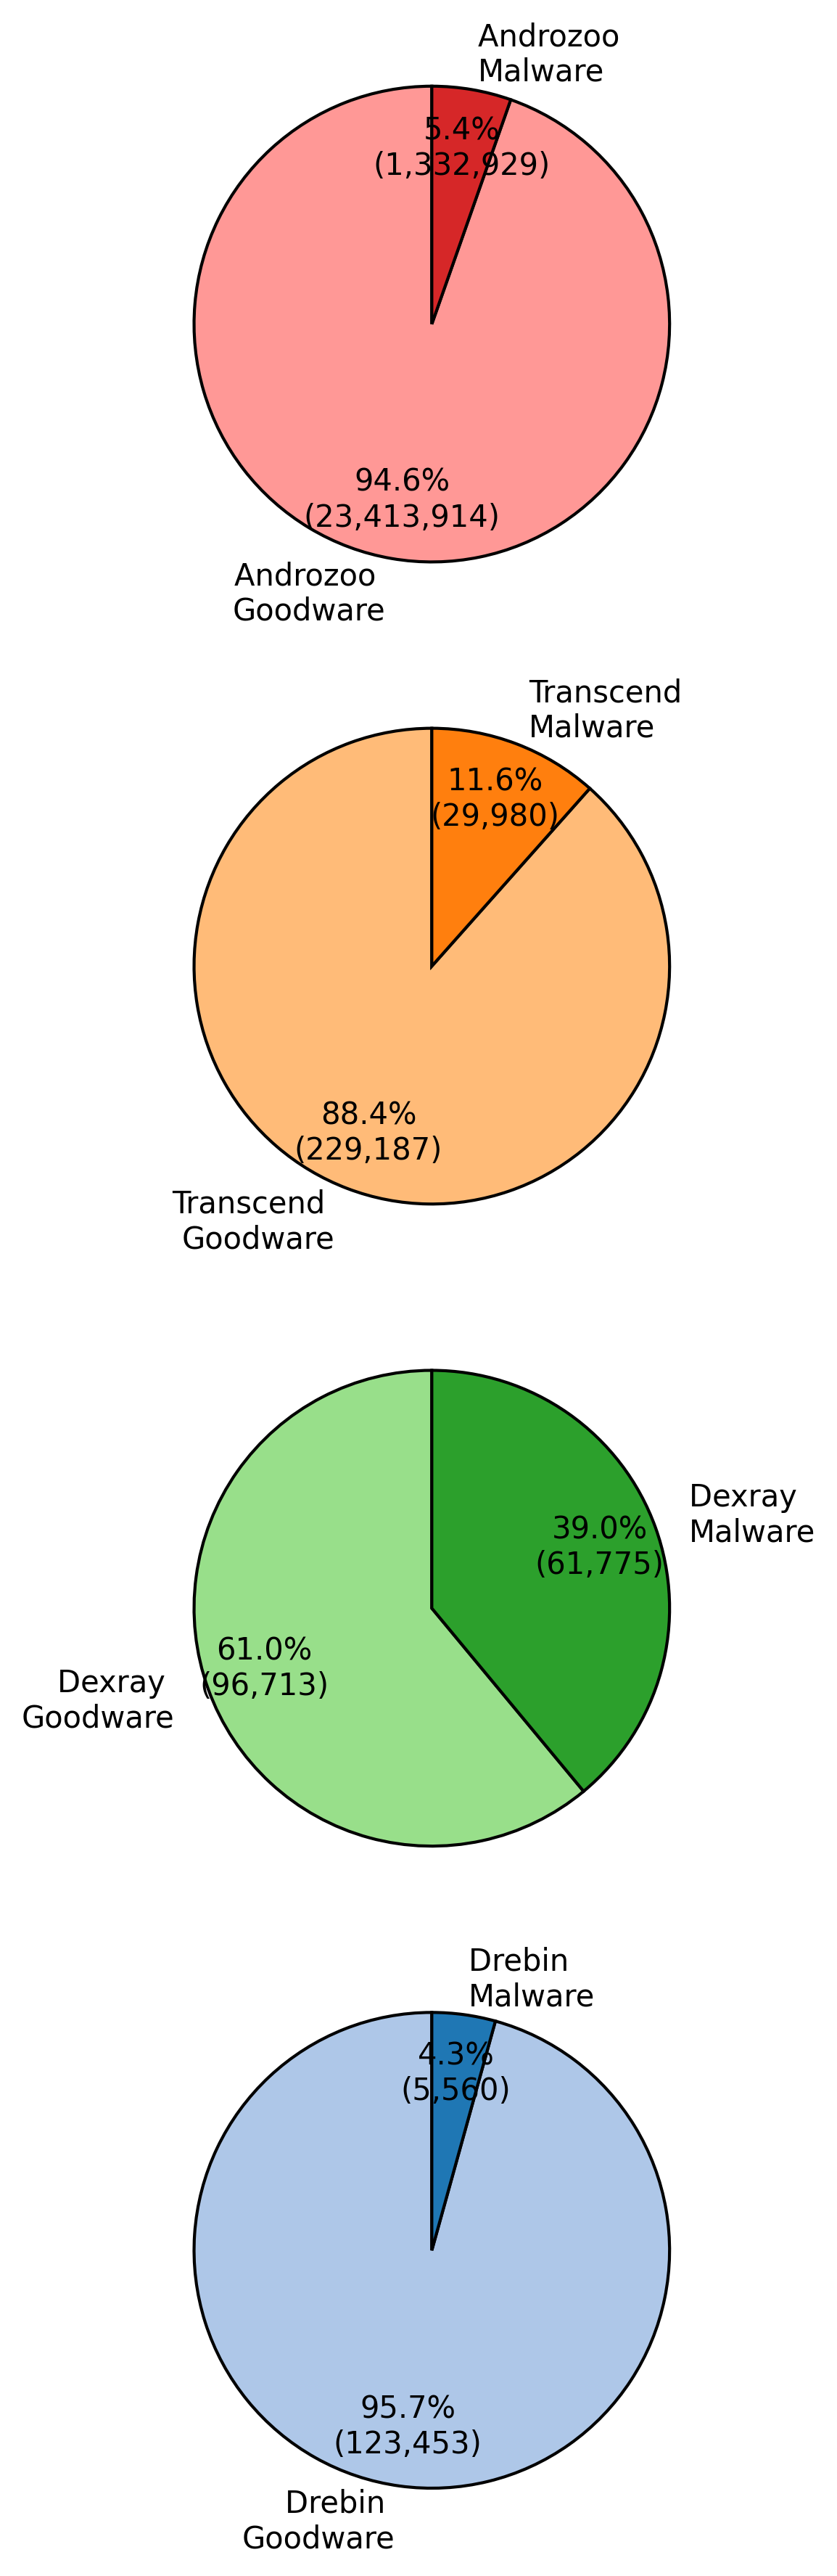
\includegraphics[width=1\marginparwidth]{3_Methodology/malware_goodware_ratios.png}
    \caption{\label{fig:malratios}
    Distribution of malware and goodware samples across datasets shown as pie charts.
    The datasets analyzed are are ordered by size from largest to smallest.
    The number of APKs contained in the Dataset are shown in brackets}
\end{marginfigure}

The evaluation of datasets forms a critical foundation for the success of any machine learning task, 
especially in security sensitive applications such as mobile malware detection. 
A robust dataset not only enables effective training of models but also ensures generalizability 
across various scenarios, including concept drift. 
This section outlines the dataset evaluation process undertaken for this research.

The datasets that are evaluated are introduced in subsection \ref{sec:amd}.
The Drebin, Transcend, and DexRay datasets are well suited for comparison because they are 
specifically designed to serve as benchmarks for training and evaluating models on android malware detection. 
Each dataset is designed to train specific models and assess their performance. 
Androzoo is notably different because it serves as a large repository for Android APKs rather 
than a closed dataset specifically designed for training and benchmarking algorithms. 
Additionally, it is continuously updated and expanded by the authors.

When comparing the number of APKs of each dataset, Androzoo has the most APKs with 25,059,602 
(as of 06.103.2025 14:23). 
Since it is a repository, it will continue to grow larger.
The biggest of the benchmarking datasets is Transcend, which has 259,230 available APKs. 
This is followed by DexRay with 159,803 APKs, and then Drebin with 129,013 APKs. 
In general, larger datasets are better for training and evaluating a model. 
However, this is only true if the dataset size correlates with novelty, 
meaning it introduces unique and diverse cases. 
For example, a dataset containing applications from various time periods or regions 
ensures that the model can generalize to unseen scenarios. 
This has been shown by \cite{scalinglaws}, 
where they demonstrated that the performance of Transformer Decoder Models 
correlates with the size of the data used to train them.

Figure \ref{fig:malratios} shows the label distribution for each dataset. 
Notably, the DexRay dataset has an unusually high percentage of malware APKs. 
On one hand, this could help the model learn more diverse representations of malicious APKs. 
On the other hand, Arp et al. refer to this as a sampling bias, where 
"the collected data does not adequately represent the true distribution of 
the underlying security problem" \cite{dodo}. 
While the actual label distribution is unknown 
(and likely changes depending on the models use case), 
it seems unlikely that 39\% of APKs are generally malware. 
Similarly, the Transcend dataset also has a high malware rate, 
with over 10\% of its samples being malicious. 
In comparison, Androzoo and Drebin show about 5\% malware APKs in their distributions. 
The Androzoo Malware labels were derived from 
virustotal\footnote{https://www.virustotal.com/gui/home/upload} by 
Euphony \cite{androzoo_malware} in 2017, 
which means that they are outdated as newer APKs were not evaluated.

%\vspace*{-2\baselineskip} % Move the figure upwards
\begin{marginfigure}[-50pt] % 't' specifies top placement
    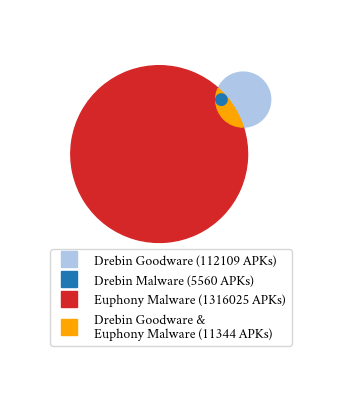
\includegraphics[width=1\marginparwidth]{3_Methodology/euphony_drebin_overlap.png}
    \caption{\label{fig:euphony_drebin_overlap}
    Overlap between the Drebin and Euphony datasets. 
    The light blue circle represents Drebin, where 112,109 APKs are classified as goodware (excluding overlap).
    The red circle represents Euphony, which contains 1,316,025 APKs labeled as malware (excluding overlap). 
    The dark blue circle represent those 5560 APKs, that are considered malware for both Drebin and Euphony.
    The intersection in orange highlights 11,344 APKs classified as goodware by Drebin but as malware by Euphony.}
\end{marginfigure}

One important aspect is that there is no clear definition of malware, 
which significantly impacts the analysis. 
This lack of a universal definition leads to inconsistencies in classification across datasets, 
making it challenging to validate labels and draw reliable comparisons. 
Without a standardized framework, each dataset might apply its own criteria.
Each dataset can have different interpretations of what is considered malware, 
often based on criteria such as the presence of specific permissions, 
API calls, or behaviors flagged by antivirus software. 
One dataset might classify an APK as malware due to aggressive adware practices, 
while another might only consider code executing malicious payloads. 
These differences make the validation of labels very difficult.
One Example that shows this issue is evident when comparing Drebin with Euphony 
(figure: \ref{fig:euphony_drebin_overlap}).
Euphony and Drebin have a common subset, none of the sets is a true subset of the other.
However, the APKs labeled as malware by Drebin are a true subset of Euphony.
Additionally, Euphony classifies multiple APKs as malware that were classified as goodware by Drebin.
The fact that there are no APKs that are classified as malware by Drebin and Goodware 
by Euphony shows that Drebin applies a more narrow definition on what is considered malware.
Further Overlaps of different Datasets are visualized in the Appendix 
(figure: \ref{fig:dataset_overlap}).

\subsection{Temporal Evaluation}

\begin{figure*}[b]
    \centering
    \begin{minipage}{1.5\textwidth}
        \centering
        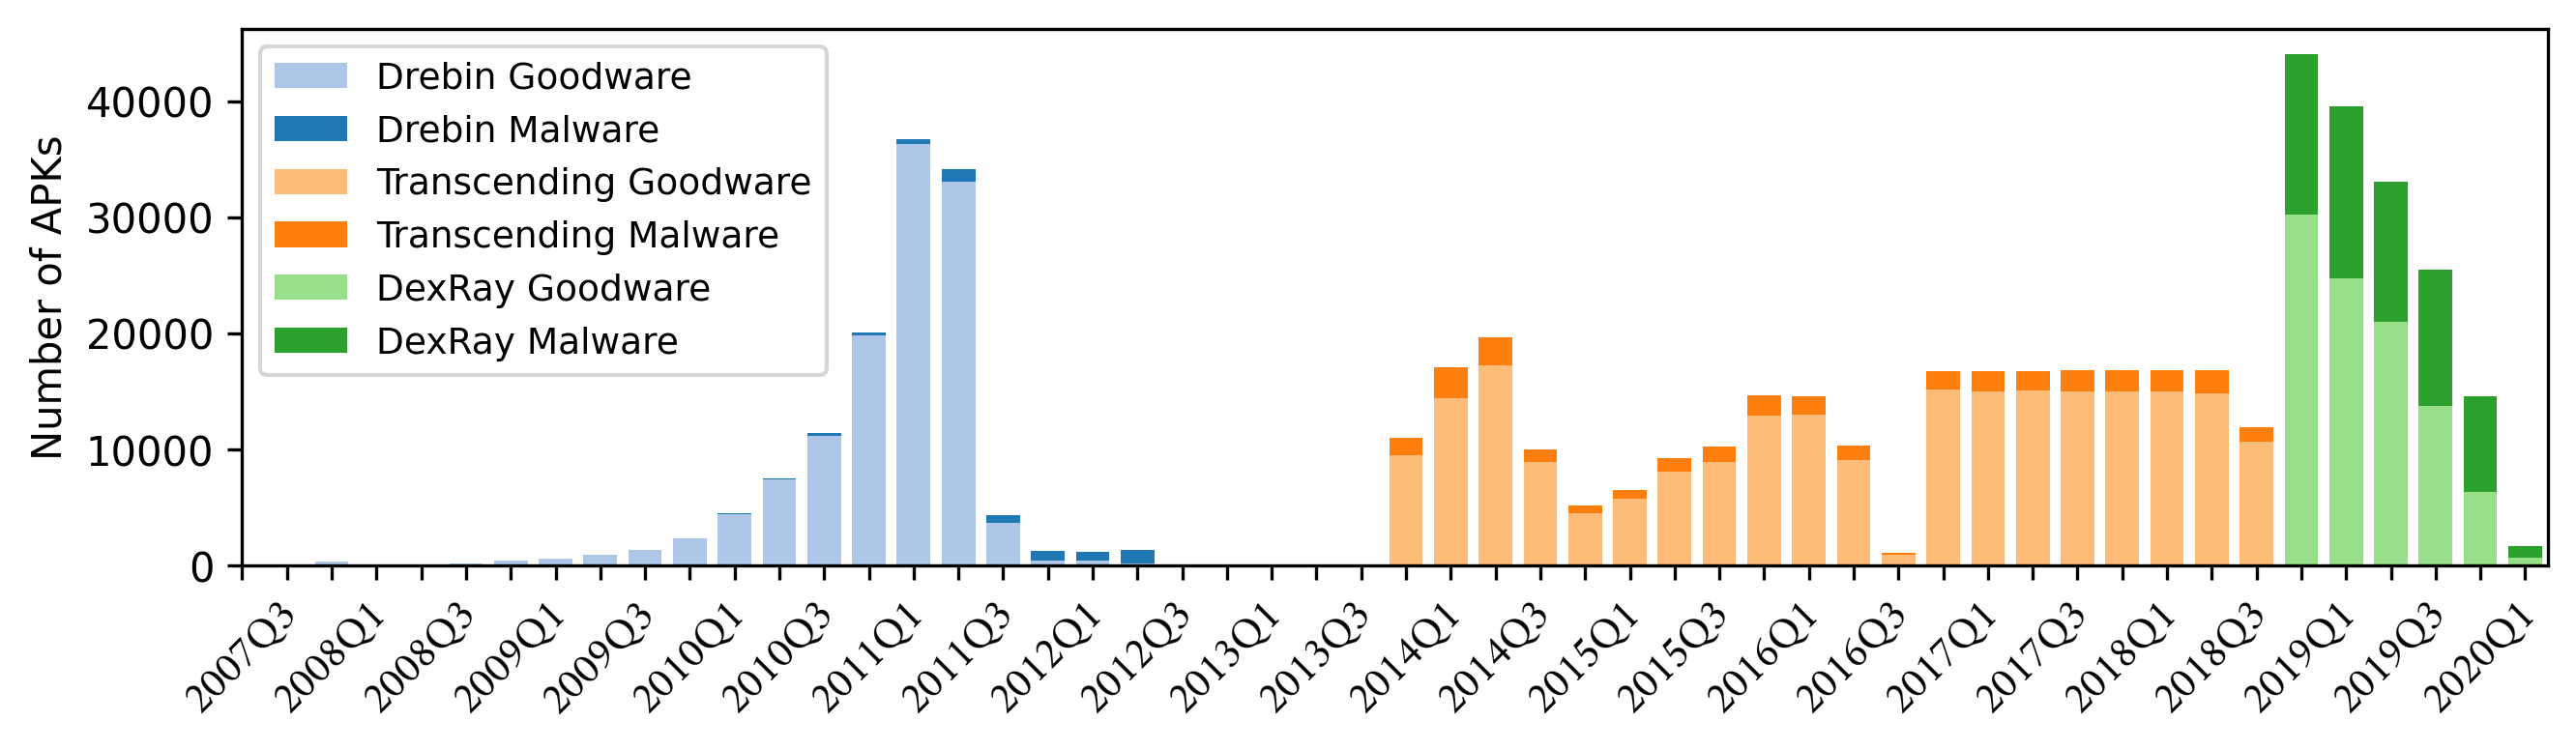
\includegraphics[width=\textwidth]{3_Methodology/dataset_time_distribution.png}
        \captionsetup{width=\textwidth}
        \caption{\label{fig:dataset_time_evaluation}
        Temporal distribution of Android APKs across three datasets (Drebin, Transcend, and DexRay), 
        categorized into goodware and malware.
        The Data is derived from metadata of the classes.dex file of each APK.
        }
    \end{minipage}
\end{figure*}

The temporal evaluation of APKs is often based on metadata of the classes.dex component, 
as it contains crucial timestamp information reflecting the compilation date of the code. 
This metadata serves as a reliable indicator of the APKs development period, 
providing a foundation for chronological analyses.
While this often works (figure: \ref{fig:dataset_time_evaluation}), 
it becomes more common that this meta information is not available. 
This lack of metadata poses challenges for temporal evaluation, 
as it limits the ability to analyze trends and shifts in malware development over time, 
as seen by the temporal evaluation of the androzoo repository 
(figure: \ref{fig:androzoo_temporal}).

The distribution of the .dex dates of the three datasets 
(figure: \ref{fig:dataset_time_evaluation}) shows that the datasets are in succession of one another. 
There is no temporal overlap, which explains why there is no APK present in more than one of 
these datasets (figure: \ref{fig:dataset_overlap}). 
There is a gap between the third quarters of 2012 and 2013 where neither dataset has samples. 

While the Transcend Dataset seems to be evenly distributed, 
the other two datasets seem to show varying volumes over time. 
This holds true for the overall volume but also about the evenness of the label distribution. 
Here Drebin and DexRay show unbalanced malware sample behavior. 
This uneven distribution can affect the generalizability of findings.

% (Extendable)
One Example where concept drift is visible is, 
that the size of packaged APKs grows with time \ref{fig:dataset_size_evaluation}.
The three datasets show different distributions of APK sizes, 
where Drebin shows the smallest and DexRay the biggest APKs on average.
The Plot also shows that the labels of all datasets are more evenly distributed by the APK size, 
compared to the .dex date of the APK.

% Nochmal Drüberlsesen:::!!!
When evaluating a model regarding the concept drift of malware, 
the Transcend dataset shows the most potential.
However, only considering one dataset limits the generalizability of an approach, 
so the evaluation on multiple datasets is even better.
One Problem is, that all three datasets only contain APKs where the .dex date is available.
The temporal evaluation of Androzoo \ref{fig:androzoo_temporal} showed that this is for most 
modern APKs not the case.
It follows that each of the datasets are Biased in their selection of APKs and are 
therefore not fit for representing the True APK landscape. 

\begin{figure*}[b!]
    \centering
    \begin{minipage}{1.5\textwidth}
        \centering
        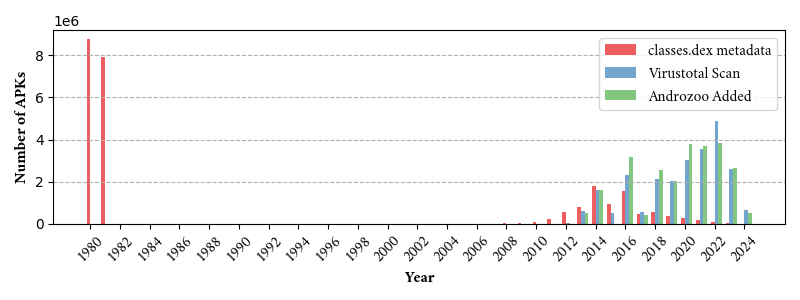
\includegraphics[width=\textwidth]{A_Images/androzoo_temporal.png}
        \captionsetup{width=\textwidth}
        \caption{\label{fig:androzoo_temporal}
        Temporal distribution of APKs based on three key attributes: 
        classes.dex metadata, Virustotal Scan, and Androzoo Added. 
        The red bars (classes.dex metadata) show a large spike in 1980 to 1982, 
        likely due to incorrect or missing metadata values. 
        The blue (year of first scan by virustotal on that APK) and 
        green (year this APK was added to the androzoo repository) bars 
        indicate a consistent increase in APK activity from 2010 onward, 
        peaking around 2020 to 2022, reflecting the growing adoption of Android 
        and corresponding malware collection efforts. 
        The discrepancies between attributes highlight potential issues in 
        dataset metadata accuracy and consistency.
        }
    \end{minipage}
\end{figure*}


\newpage

\subsection{Code Evaluation}

When checking for Malware, an important representation of an APK is its code.
As the code describes the logic of what the App does, it seems logical that, if the 
code is sufficiently evaluated, the harmfulness of the APK can be derived.
Especially Transformer models show promise in interpreting the code of an APK as they work very well as LLMs.

It follows that not just time distributions of the datasets should be evaluated, but also the distribution of code.
There are two major ways of decompiling an APK into a code representation.
The classes.dex file can either be decompiled into Java code or into lower level Smali code.

For the decompilation of the APK into Java code, dex2jar\footnote{https://github.com/pxb1988/dex2jar} is first used to decompile the classes.dex file into a JAR file.
The JAR file can then be further decompiled into plain Java code. 
The resulting Java code is on the one hand easy to interpret due to its higher level nature, 
however the decompiled code is prone to obfuscation that can make it hard to interpret.
One example on how obfuscation can make the logic of the App more complex is by changing the package names, 
so that it is not possible to see the entry points that are defined in the Manifest file. 
This phenomenon is further evaluated in tables \ref{tab:matching_java_classes_transcend} and \ref{tab:matching_java_classes_dexray} in section
\ref{sec:tran_enc}.

There also is an option to decompile the classes.dex file into Smali code.
Smali is the human readable representation of the Dalvik bytecode that is found in the raw classes.dex file.
Smalie therefore is to Dalvik bytecode, what Assambly is to machine code.
The Smali representation of an APK can be retrieved by using Apktool\footnote{https://apktool.org/} on the classes.dex file.
While the Smali representation is more accurate the original bytecode and also is more robust to obfuscation, 
the readability is much harder due to the lower level and niche nature.

\begin{figure*}[b!]
    \centering
    \begin{minipage}{1.5\textwidth}
        \centering
        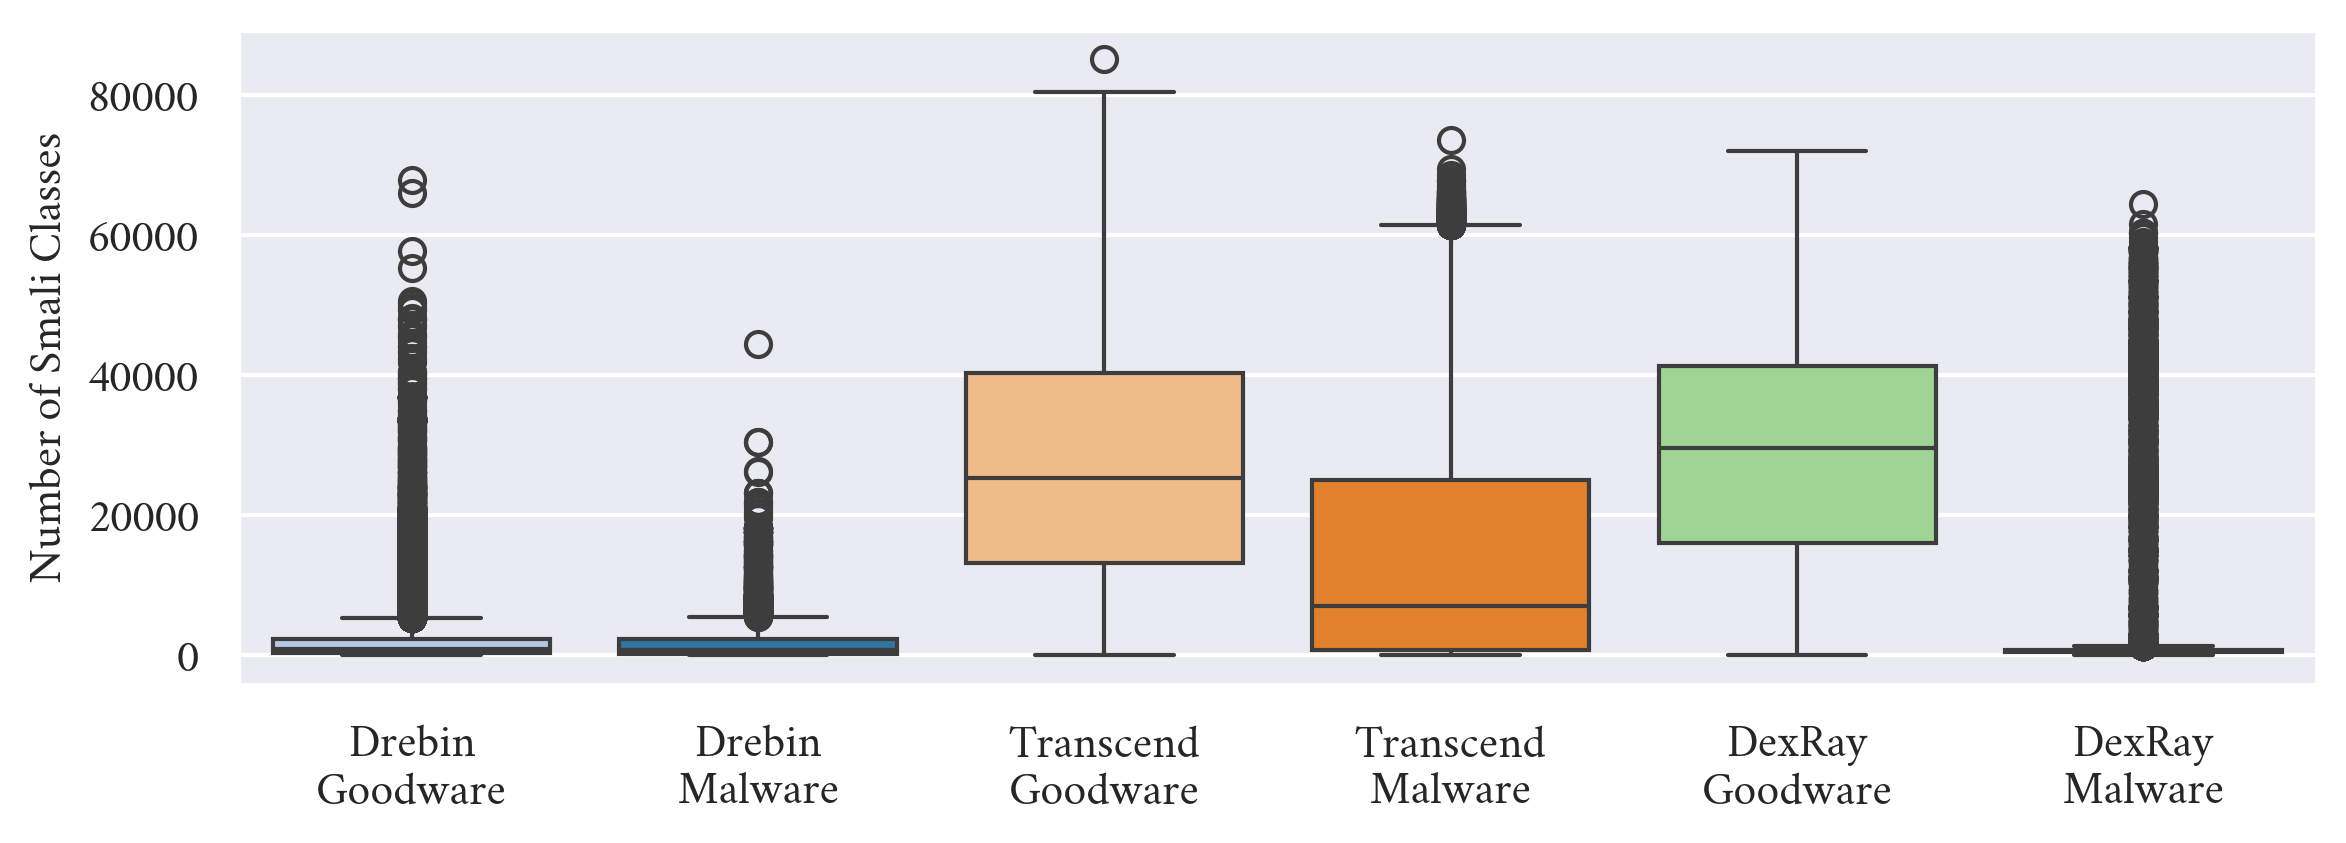
\includegraphics[width=\textwidth]{3_Methodology/smali_class_boxplots.png}
        \captionsetup{width=\textwidth}
        \caption{\label{fig:smali_class_boxplots}
        The boxplot shows the distribution of Smali classes in Android apps 
        across the Drebin, Transcend, and DexRay datasets, 
        split into Goodware and Malware. 
        Drebin and Transcend have an similar Smali class distribution 
        between Goodware and Malware.
        The DexRay Dataset shows a high inbalance in the number of Smali classes 
        between the two labels.
        }
    \end{minipage}
\end{figure*}

\newpage

\begin{margintable}[1\baselineskip] % Move table down by 1 line
    \caption{\label{tab:smali_distribution}Smali Statistics Summary for DexRay, Transcend, and Drebin.}
    \footnotesize
    \begin{tabular}{@{}lccc@{}}
        \toprule
        \tabhead{Label} & \tabhead{Q1} & \tabhead{Median} & \tabhead{Q3} \\
        \midrule
        \multicolumn{4}{l}{\textbf{DexRay}} \\
        Goodware & 16106 & 29546 & 41352 \\
        Malware & 445 & 598 & 817 \\
        \midrule
        \multicolumn{4}{l}{\textbf{Transcend}} \\
        Goodware & 13145 & 25364 & 40372 \\
        Malware & 764 & 7057 & 25015 \\
        \midrule
        \multicolumn{4}{l}{\textbf{Drebin}} \\
        Goodware & 331 & 901 & 2353 \\
        Malware & 173 & 805 & 2316 \\
        \bottomrule
    \end{tabular}
\end{margintable}

As part of the code evaluation of this thesis, 
the same three datasets as in the time evaluation were considered.
For each APK of the datasets, the classes.dex file was decompiled 
in both an Java and an Smali code representations.
The code representation of an APK is quite complex and only hardly allows 
statistical aalysis.
One approach that was possible is to count the classes of the code representations for each APK,
reducing the complexity from a repository per app to a number.
Figure \ref{fig:smali_class_boxplots} shows the Boxplots of the distribution 
of Smali classes of the apps in the dataset distinguishing 
between the label of the APK.
The Boxplots show, that Drebin has a generally low amount of Smali classes 
per APK, wich can be explained by the Apps being 
older (as shown in table \ref{fig:dataset_time_evaluation}) and 
smaller (as shown in table \ref{fig:dataset_size_evaluation}) than those of the other datasets.

A second observation, is that the DexRay Dataset is highly inbalanced.
This is apparent both from the Boxplot (figure \ref{fig:smali_class_boxplots}) and also by table \ref{tab:smali_distribution},
that quantifies the distribution of smali classes by computing the Q1, Median and Q3 values of each of the Datasets.
When looking further into \ref{tab:smali_distribution} the issue becomes even more apparent. 
Q1, Median and Q3 differ between the labels by a factor of 35-50, this makes any approach that makes label 
predictions based on Smali code of that dataset questionable (for example \cite{dexbert,detectbert,dexray}).

\begin{margintable}[1\baselineskip] % Move table down by 1 line
    \caption{\label{tab:java_distribution}Java Statistics Summary for Drebin, Transcend, and DexRay.}
    \footnotesize
    \begin{tabular}{@{}lccc@{}}
        \toprule
        \tabhead{Label} & \tabhead{Q1} & \tabhead{Median} & \tabhead{Q3} \\
        \midrule
        \multicolumn{4}{l}{\textbf{Drebin}} \\
        Goodware & 19 & 60 & 176 \\
        Malware & 18 & 66 & 224 \\
        \midrule
        \multicolumn{4}{l}{\textbf{Transcend}} \\
        Goodware & 854 & 1800 & 2899 \\
        Malware & 52 & 738 & 2244 \\
        \midrule
        \multicolumn{4}{l}{\textbf{DexRay}} \\
        Goodware & 1035 & 2007 & 3084 \\
        Malware & 7 & 11 & 11 \\
        \bottomrule
    \end{tabular}
\end{margintable}


The Transcend dataset shows less inbalance in code volume compared to the DexRay dataset.
Especially on Q1 differs by a factor of 17,2 showing that there are relatively more code sparse Malware than Goodware APKs.
When comparing the upper end of the spectrum, the inbalance becomes less drastic with an factor of ~3,5 for the median and 1,6 for the Q3.
Drebin shows overall a very good inbetween class balance of Smali classes when compared to the other datasets.

The decompilation into Java classes paints a similar picture. 
For comparison there is a similarly structured table showing the statistical properties of the Java class distribution \ref{tab:java_distribution}.
Additionally in the Appendix (\ref{sec:appendiximages}) there is another Boxplot \ref{fig:java_class_boxplots} that has the same 
structure as figure \ref{fig:smali_class_boxplots}.
When evaluating the volume of Java and Smali classes over all datasets a correlation coefficient of 0.92 proofs that they are very similar.

Table \ref{tab:java_distribution} shows that for the DexRay Dataset, more than 75\% of the malware APKs have less than 12 Java classes, 
while 75\%  of the goodware labeled ones have more than 1000 Java classes.
This makes it highly likely that an classifier will just differentiate 
between the number of classes present and derive the prediction from this information.
This leads to the conclusion, that the DexRay dataset is generally insufficient for training a code based classifier.


\section{Baseline Creation}
\label{sec:baseline}

When generating a baseline for mobile malware detection, concept drift hast to be considered.
Jordaney et al. \cite{transcend} showed that there is a concept drift for android malware.
In order to train a model that is robust again this concept drift, 
Kan et al. \cite{tesseract} propose to split the data into train and test data in a particular way.
The training data should be from before the test data, 
while keeping the same label ratio in between splits.  
The reason for this is to make sure that the model does not train on features of the data, 
that are prone to concept drift.
The punishment for this is maximized if the train and test data is sequential.
In order to account for and validate the concept drift in the domain of malware detection,
the following baselines where both created on a dataset that is split randomly into train and test subsets
and also split time based as proposed by \cite{transcend}.
The data is split into 80\% test and 20\% train data for both splitting Approaches.
The evaluation is always done in a balanced manner, penalizing mistakes on the less frequent malware label more.

\subsection{Non Transformer Approaches}

\begin{table*}[t!]
    \begin{minipage}{1.5\textwidth}
        \captionsetup{width=\textwidth}
        \caption{\label{tab:treestump} Tree Stump (balanced class weights) results by dataset, feature, and split.}
    \end{minipage}
    \small
    {\renewcommand{\arraystretch}{1.5} % Increase row height for better readability
        \begin{tabularx}{\linewidth}{@{}l l l r r r r r@{}} % Adjusted alignment: l for text, r for numbers
            \toprule
            \textbf{Dataset} & \textbf{Feature} & \textbf{Split} & \textbf{Accuracy} & \textbf{Precision} & \textbf{Recall} & \textbf{F1 Score} & \textbf{Threshold} \\
            \midrule
            Drebin & Java classes & random     & 10.16\% & 4.40\% & 99.07\% & 8.43\% & 2.5 \\
                   & Java classes & time based & 7.39\%  & 4.31\% & 96.49\% & 8.24\% & 3.5 \\
                   & Smali classes & random    & 76.01\% & 6.14\% & 33.24\% & 10.37\% & 247.5 \\
                   & Smali classes & time based & 7.15\%  & 4.31\% & 96.76\% & 8.24\% & 33.5 \\
                   & APK size     & random     & 10.94\% & 4.32\% & 96.10\% & 8.27\% & 59676 \\
                   & APK size & time based & 6.62\%  & 4.35\% & 98.38\% & 8.33\% & 59676 \\
            \midrule
            Transcend & Java classes & random     & 90.05\% & 70.58\% & 23.38\% & 35.12\% & 17.5 \\
                         & Java classes & time based & 82.63\% & 36.58\% & 68.35\% & 47.65\% & 967.5 \\
                         & Smali classes & random    & 77.63\% & 27.44\% & 57.28\% & 37.10\% & 9699.5 \\
                         & Smali classes & time based & 77.61\% & 31.23\% & 77.85\% & 44.58\% & 15101.5 \\
                         & APK size     & random     & 18.75\% & 11.90\% & 94.56\% & 21.14\% & 57904190 \\
                         & APK size & time based & 39.27\% & 11.77\% & 65.44\% & 19.96\% & 11054373 \\
            \midrule
            DexRay & Java classes & random     & 92.05\% & 93.04\% & 86.37\% & 89.58\% & 90.5 \\
                   & Java classes & time based & 94.74\% & 89.67\% & 97.65\% & 93.49\% & 90.5 \\
                   & Smali classes & random    & 92.10\% & 93.19\% & 86.36\% & 89.64\% & 1395.5 \\
                   & Smali classes & time based & 94.59\% & 89.35\% & 97.63\% & 93.31\% & 1395.5 \\
                   & APK size     & random     & 48.53\% & 42.97\% & 91.97\% & 58.58\% & 79432704 \\
                   & APK size & time based & 44.78\% & 39.11\% & 76.98\% & 51.87\% & 67843648 \\
            \bottomrule
        \end{tabularx}
    }
\end{table*}

A very simple classifier is a decision tree stump.
This stump is infering a threshold based on the training data and then using it to predict a label for new samples.
To make it even simpler for creating a first baseline, in Table \ref{tab:treestump} only one feature is considered when calculating the tree stump.
The table shows how the Drebin dataset is most robust to this very basic approach.
For Drebin, neither of the considered features (Number of Java classes, Number of Smali classes \& Size of the packaged APK)
is fit for successfully separating the labels with one threshold.
On the first glance it seems unlikely, that the thresholds for the APK sizes are constant over both different dataset splits.
Since the threshold is changing for some other random splits (by using other random seeds),
this phenomenon seems to be due to chance.
This can be explained by how the threshold is derived from the training data
using the gini coefficient \cite{gini}.

On the Transcend dataset, the Tree Stump approach achieve better results.
Here the concept drift can be observed by the changing thresholds between the split methods.

The most shocking result is, that the DexRay dataset can be solved with an F1 score of 93,49\% 
with a simple Tree stump approach on the Java classes feature.
This shows how inbalanced the dataset is and how it is unfit for evaluatig models 
that rely on code based features.
Another interesting observation is that for both the Java and the Smali classes the 
Thresholds stay consistent inbetween different splits of the data.
Also the performance increases when the data is split based on time rather than randomly, 
which means that the newest APKs are most prone to this label inbalance.

Overall the table \ref{tab:treestump} shows how different the datasets are, 
even though all of them are build for the same objective of evaluating android malware 
detection models.
The same model achieves an F1 score of 8\% on Drebin, 48\% on Transcend and 93\% on DexRay.

\begin{table}[t]
    \caption{\label{tab:randomforest}%
    Random Forest (n\_estimators=300, max\_depth=25) results by dataset and split. Features include Java classes, Smali classes, and APK Size.}
    \resizebox{\textwidth}{!}{%
    \begin{tabular}{@{}llcccc@{}} % Removes outer horizontal margins
    \toprule
    \textbf{Dataset} & \textbf{Split} & \textbf{Accuracy} & \textbf{Precision} & \textbf{Recall} & \textbf{F1 Score} \\ \cmidrule(r){1-2} \cmidrule(lr){3-6}
    Drebin         & random     & 98.08\% & 91.69\% & 59.42\% & 72.11\% \\
                   & time based & 95.66\% & 48.69\% & 13.40\% & 21.02\% \\ \addlinespace
    Transcend   & random     & 94.53\% & 88.74\% & 60.19\% & 71.73\% \\
                   & time based & 90.07\% & 60.47\% & 40.94\% & 48.83\% \\ \addlinespace
    DexRay         & random     & 96.87\% & 97.75\% & 94.25\% & 95.97\% \\
                   & time based & 93.95\% & 87.34\% & 98.63\% & 92.64\% \\
    \bottomrule
    \end{tabular}%
    }
\end{table}

Applying a more sophisticated model on all three of the features, increses the performance further.
This can be shown by evaluating a decision tree (table \ref{tab:decisiontree}) or a generally higher performing random forest (table \ref{tab:randomforest}) model. 
Table \ref{tab:randomforest} shows how a random forest algorithm achieves around 70\% F1 score on Drebin and Transcend when 
trained and tested with the randomly split data.
The concept drift of both Drebin and Transcend becomes apperent by lower performance on the time based split data.
Here Drebin shows an even steeper decline compared to Transcend showing more concept drift in the data.
When evaluating the random forest on DexRay, both the random and time based splits show a very high F1 score of 92\%-96\%.
it is noteworthy that a tree stump on either Java or Smali classes (table \ref{tab:treestump}) performs better than the random forest on the time based split data.
This shows that the relatively simple random forest model already overfits the time based training data.

Another possible representation of android APKs is by the permissions listed in the manifest file.
This representation too can be used to classify the APK as malicious.
Table \ref{tab:decisiontreepermissions} shows however that a decision tree trained on only these features 
performs worse than the random forest on only the three previous features.
This shows how valuable code based features are for malware detection.

When combining the permissions, the code volume features and the APK size feature, 
a decision tree outperforms the random forest that is trained without considering permissions (see table \ref{tab:decisiontreecombined}).
By then also increasing the model complexity through the depth hyperparameter from 15 to 30, 
the highest non transformer baseline of this work is achieved (see table \ref{tab:decisiontree30}).
The table shows once more how the time based split leads to worse performance for all three datasets, 
so that concept drift is apparent and generalizability of the approach is questionable.
Other than being prone to concept drift, the results show that the performance on Drebin and Transcend is not satisfactionary.

On a general level the very basic models that have been evaluated on the three datasets showed that
each dataset exhibits some form of concept drift, shown by decreasing performance when splitting the dataset based on time.
Also the DexRay dataset has such a big label inbalance on the code volume features that a simple tree stump nearly solves the dataset, 
this renders the dataset not sufficient for evaluating code based models.
    
\begin{table}[t]
    \caption{\label{tab:decisiontreepermissions}%
    Decision Tree (max\_depth=15) results by dataset and split. Features include Permissions.}
    \resizebox{\textwidth}{!}{%
    \begin{tabular}{@{}llcccc@{}}
    \toprule
    \textbf{Dataset} & \textbf{Split} & \textbf{Accuracy} & \textbf{Precision} & \textbf{Recall} & \textbf{F1 Score} \\ \cmidrule(r){1-2} \cmidrule(lr){3-6}
    Drebin         & random     & 95.74\% & 49.77\% & 90.17\% & 64.14\% \\
                   & time based & 87.60\% & 24.83\% & 92.54\% & 39.15\% \\ \addlinespace
    Transcend   & random     & 78.03\% & 32.79\% & 85.77\% & 47.44\% \\
                   & time based & 72.26\% & 26.17\% & 76.91\% & 39.05\% \\ \addlinespace
    DexRay         & random     & 90.25\% & 87.34\% & 88.07\% & 87.70\% \\
                   & time based & 83.66\% & 71.80\% & 95.01\% & 81.79\% \\
    \bottomrule
    \end{tabular}%
    }
\end{table}
    
\begin{table}[b!]
    \caption{\label{tab:decisiontree30}%
    Decision Tree (max\_depth=30) results by dataset and split. Features include Java classes, Smali classes, APK Size, and Permissions.}
    \resizebox{\textwidth}{!}{%
    \begin{tabular}{@{}llcccc@{}}
    \toprule
    \textbf{Dataset} & \textbf{Split} & \textbf{Accuracy} & \textbf{Precision} & \textbf{Recall} & \textbf{F1 Score} \\ \cmidrule(r){1-2} \cmidrule(lr){3-6}
    Drebin         & random     & 98.58\% & 81.41\% & 86.04\% & 83.66\% \\
                   & time based & 94.89\% & 45.17\% & 86.96\% & 59.45\% \\ \addlinespace
    Transcend   & random     & 95.03\% & 76.65\% & 82.03\% & 79.25\% \\
                   & time based & 92.21\% & 65.16\% & 69.95\% & 67.47\% \\ \addlinespace
    DexRay         & random     & 96.95\% & 96.36\% & 95.89\% & 96.13\% \\
                   & time based & 94.88\% & 89.14\% & 98.78\% & 93.72\% \\
    \bottomrule
    \end{tabular}%
    }
\end{table}
    
    
\newpage  

\subsection{DetectBERT}
\label{sec:detectbert}

\begin{figure*}[b]
    \centering
    \begin{minipage}{1.5\textwidth}
        \centering
        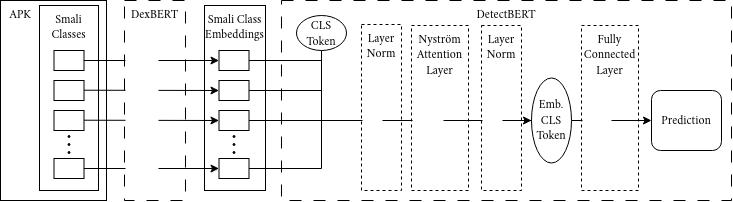
\includegraphics[width=\textwidth]{3_Methodology/detectbert_schema.png}
        \captionsetup{width=\textwidth}
        \caption{\label{fig:detectbert_schema}
        Overview of the DetectBERT architecture. 
        The model processes APK files by extracting small class representations using DexBERT, 
        which generates embeddings for each class. 
        A CLS token is added to the sequence, 
        followed by layer normalization and a Nyström attention layer. 
        Additional layer normalization is applied before feeding the CLS token embedding 
        into a fully connected layer to generate the final prediction.
        }
    \end{minipage}
\end{figure*}


In the previous chapters, various non Transformer based approaches for 
static Android malware detection were explored. 
These methods rely on traditional machine learning techniques and therefore  
struggle with capturing the complex relationships within Android application data. 
In contrast, Transformer based models have demonstrated SOTA 
performance in various NLP and code understanding tasks \cite{transformer_sota}. 
This chapter introduces DetectBERT \cite{detectbert}, the first Transformer-based approach examined 
in this thesis.

DetectBERT is a static Android malware detection model that utilizes Transformer based architectures for analyzing APK files.
Its processing schema is visualized in figure \ref{fig:detectbert_schema}.
Specifically, DetectBERT processes the classes.dex file contained within Android APKs by extracting Smali class representations. 
These representations are subsequently transformed into compact feature embeddings using DexBERT \cite{dexbert}, 
a specialized Transformer model developed by the same authors for this task.
These embeddings serve as inputs to the DetectBERT component, a Transformer architecture that employs Nyström based attention \cite{nystromformer} 
to effectively manage computational complexity while capturing long-range dependencies. 
The embeddings, together with a special CLS token, designed to aggregate global context, are refined through successive layer normalization and Nyström attention layers. 
This processing aims for, global feature representation encapsulated in the embedding of the CLS token.
Finally, DetectBERT uses a fully connected  layer to process the Embedded CLS token into a  malware prediction, indicating whether the APK is malicious or benign.

To evaluate DetectBERT, we benchmarked its performance on the DexRay ad Transcend datasets. 
Due to computational and time constraints, the full DexRay and Transcend datasets were not used. 
Instead, subsets of both datasets were generated, each containing 20,000 APKs with an even label distribution. 
Additionally, the Smali class distributions were balanced between malware and 
goodware samples, countering the inherent imbalance of the DexRay dataset. 
The DexRay dataset is also the dataset that was used for benchmarking the model 
in its original paper. However, due to the Smali class imbalance between labels, 
the benchmarks presented in the paper were not entirely trustworthy. 
The results on the balanced subset do indicate, that the model does not simply rely 
on the number of Smali classes for predictions but at least to some extent, 
utilizes other information extracted from the Smali class embeddings. 
However, the results on the subsets are not as good as those provided in the 
original paper (see Table \ref{tab:detectbert_performance_original}). 
This performance discrepancy might also be attributed 
to the smaller training dataset size used in our experiments.

The model was tested under two different data splitting strategies: a random split, 
which ensures a balanced distribution of samples in training and testing, 
and a time based split, which simulates realworld conditions by training on older 
data and testing on newer samples. 
Table \ref{tab:detectbert-results} presents the detection performance of DetectBERT across both datasets 
and splits. The results indicate that DetectBERT is
achieving high accuracy and F1 scores, particularly on the DexRay dataset. 
The model demonstrates a slight decline in performance for time-based splits, 
likely due to evolving malware patterns. 
The performance on the subset of the Transend dataset are not as good as 
on the DexRay dataset.

The evaluation gives several key insights about DetectBERTs performance. 
Transformer based models effectively capture complex relationships in APK data, 
surpassing traditional methods for the Transcend dataset (see table \ref{tab:decisiontree30}). 
The DexRay dataset yields better results compared 
to Transcend, suggesting dataset specific challenges. 
The time based split introduces a more realistic evaluation setting, 
exposing the impact of concept drift in malware evolution.

Overall, DetectBERT is implemented as a TransMIL model , which is a Transformer based 
multiple instance learning (MIL) framework \cite{transmil}. 
In this approach, the model processes 
multiple Smali class embeddings as instances within an APK and learns to make a 
classification decision based on the most relevant instances. This allows DetectBERT 
to focus on the most informative Smali class embeddings rather than relying on 
simple aggregate statistics, improving its ability to detect malware patterns effectively.

\begin{margintable}[-30\baselineskip]
    \caption{\label{tab:detectbert_performance_original} DetectBERT Performance Results (accuracy, precision, recall, F1 Score) from the original paper \cite{detectbert}}
    \footnotesize
    \begin{tabular*}{\linewidth}{@{\extracolsep{\fill}} cccc@{}}
        \toprule
        \textbf{Acc.} & \textbf{Prec.} & \textbf{Rec.} & \textbf{F1} \\
        \midrule
        97\% & 98\% & 95\% & 97\% \\
        \bottomrule
    \end{tabular*}
\end{margintable}




\begin{table}[]
    \caption{\label{tab:detectbert-results}%
        DetectBERT Benchmark Results Across Datasets and Splits.  
        The results are reported for both random and time-based splits, 
        highlighting the effectiveness of the model in distinguishing between 
        goodware and malware. 
        On the DexRay dataset, DetectBERT consistently achieves higher accuracy, 
        particularly for goodware classification.}
    \resizebox{\textwidth}{!}{%
    \begin{tabular}{@{}llcccc@{}}
    \toprule
    \textbf{Dataset} & \textbf{Split} & \textbf{Accuracy} & \textbf{Precision} & \textbf{Recall} & \textbf{F1} \\ \cmidrule(r){1-2} \cmidrule(lr){3-6}
    DexRay (Subset)  & Random     & 89.57\% & 89.57\% & 89.57\% & 89.57\% \\
                     & Time-based & 89.17\% & 90.00\% & 89.17\% & 89.10\% \\ \addlinespace
    Transcend (Subset) & Random     & 81.77\% & 82.46\% & 81.77\% & 81.77\% \\
                       & Time-based & 78.67\% & 78.73\% & 78.67\% & 78.68\% \\
    \bottomrule
    \end{tabular}%
    }
\end{table}

\newpage

\section{Experimntal Setup}

\subsection{General BERT based approach}

\begin{figure*}[b]
    \centering
    \begin{minipage}{1.5\textwidth}
        \centering
        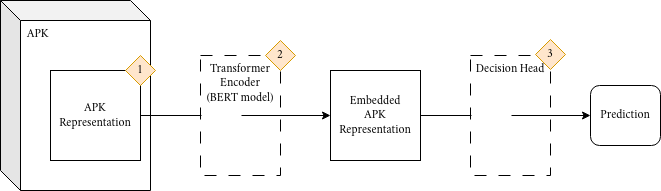
\includegraphics[width=\textwidth]{3_Methodology/bertbased_malwaredetection_schema.png}
        \captionsetup{width=\textwidth}
        \caption{\label{fig:bertbased_malwaredetection_schema}
        Generalized BERT-based approach for malware detection. 
        This figure illustrates a blueprint for utilizing BERT models in APK-based 
        malware detection. 
        The process consists of three main stages: 
        extracting an APK representation [1], 
        encoding it using a Transformer based model (BERT) [2], 
        and applying a decision head to generate the final prediction [3]. 
        The numbered elements indicate open design choices within this blueprint.
        }
    \end{minipage}
\end{figure*}

The experiments conducted in this thesis build upon a generalized paradigm 
for malware detection, as visualized 
in figure \ref{fig:bertbased_malwaredetection_schema}. 
The core idea is that, in order to classify an APK as malicious or benign, 
it must first be processed through a structured pipeline.

The first step [1] involves extracting an appropriate representation of the APK. 
This representation serves as the input for the subsequent stages 
and can be derived from different static attributes of the APK, 
ensuring that relevant structural and behavioral information is preserved.

Next, in step [2], this representation undergoes an embedding process. 
The embedding is designed to transform the extracted representation into 
a format suitable for processing further while maintaining essential 
information and reducing dimensionality. 
The choice of embedding strategy significantly influences the quality 
of the learned representation and consequently, the detection performance.

In the final step [3], the embedded representation is passed to a 
decision head that generates the final classification. 
The decision head can take various forms, from simple fully connected layers
to more complex Transformer based network structures. 
The effectiveness of the decision head plays a crucial role in 
ensuring that the model correctly distinguishes between benign 
and malicious applications.

The objective of this thesis is to analyze the capabilities of 
this architecture by systematically evaluating each of these three 
core components. By designing experiments that focus on variations 
in APK representation, embedding methods, and decision heads, 
the study aims to provide insights into the strengths and limitations 
of Transformer based malware detection models. 
The following chapters will further explore each of these stages in detail, 
discussing alternative design choices and their impact on detection performance.

\chapter{Evaluation}

\label{Evaluation} % For referencing the chapter elsewhere, use \ref{Chapter1}


\section{The APK Representation}
\label{sec:apkrepresentation}

\begin{marginfigure}[3\baselineskip] % move figure up by 1 line -5\baselineskip
    \center
    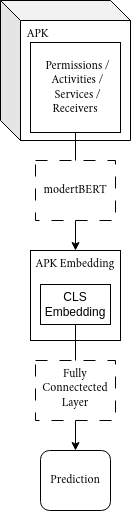
\includegraphics[width=0.6\marginparwidth]{4_Evaluation/permission_transformer_schema.png}
    \caption{\label{fig:permission_transformer_schema}
    Distribution of malware and goodware samples across datasets shown as pie charts.
    The datasets analyzed are are ordered by size from largest to smallest.
    The number of APKs contained in the Dataset are shown in brackets}
\end{marginfigure}

A key aspect of designing an embedding based mobile malware detection system is 
how the APK is represented. Since most embedding models, including all considered BERT models, 
cannot process APKs as a whole, specific features such as permissions, API calls, 
or manifest attributes must be selected and represented in a tokenizable format. 
These features should be structured consistently to ensure comparability across different APKs.

To structure these features, concatenating them with designated tokenizer vocabulary entries 
as separators is beneficial. 
In this work, a varying number of \# characters were used as separators, 
with different separators applied to distinguish between various types of separations 
(e.g., separating feature categories versus separating elements within a feature list).

To show how varying APK representations change the performance of a malware detection 
architecture, an experiment was done with a relatively simple stack 
\ref{fig:permission_transformer_schema}. 
To best see how the representation has an effect, 
the other two variables of the stack were kept static. 
For simplicity and efficiency, the selected embedder was ModernBERT \cite{modernbert}. 
Since ModernBERT has a context window of up to 8000 tokens, 
it was possible to process each APK in one iteration, 
ensuring that the entire representation was captured in a single pass. 
This approach improves efficiency by reducing computational overhead and helps preserve 
relationships within the APKs extracted features. 
The embedding size was set to 768, as recommended by the original ModernBERT authors. 
After applying the Embedding, each input token along a blank CLS token is represented
by 768 floating points.
After each APK was embedded, a simple fully connected layer with dropout was 
trained for 5 epochs on the timebased 
split subset of the dataset, as described in the previous chapter. 
To simplify processing, the decision head was not trained on the full 
embedding but rather only on the CLS token embedding. Each APK was therefore 
represented by 768 floating-point values, ensuring a compact yet 
informative representation for classification.
During training, only the weights of the last fully connected layer were updated, 
while the weights of the ModernBERT embedder were frozen.
The fully connected layer was chosen for its simplicity and effectiveness in 
classification tasks, while the dropout mechanism was included to help prevent overfitting 
and improve generalization. With this stack, 
multiple different APK representations could be chosen. 
However, the representation was limited to 8000 tokens so that it could be 
processed by ModernBERT in a single pass. 
The representations that were chosen were all extracted from the manifest.xml file, 
as it contains important metadata about an application's permissions, activities, services, 
and broadcast receivers, which are often indicative of its behavior and potential security risks. 
The selected ones were the names of the given permissions of the APK, 
the names of the marked activities, 
and the names of the marked services and receivers. 
Permissions indicate what resources an application can access, 
while activities, services, and receivers help determine its execution behavior. 

\begin{table}[b!]
    \caption{\label{tab:apk_representation_results}%
    Performance of different APK representations using frozen ModernBERT embeddings. Features are extracted from Android manifest.xml (A=Activities, P=Permissions, R=Receivers, S=Services). Results reported on time-based transcend subset split after five epochs.}
    \resizebox{\textwidth}{!}{%
    \begin{tabular}{@{}lcccc@{}}
    \toprule
    \textbf{Representation} & \textbf{Accuracy} & \textbf{Precision} & \textbf{Recall} & \textbf{F1} \\ 
    \cmidrule(r){1-1} \cmidrule(lr){2-5}
    A + P + R + S & 74.45\% & 76.30\% & 70.58\% & 73.33\% \\
    A + P + S      & 74.67\% & 76.39\% & 71.09\% & 73.64\% \\
    A + P          & 74.47\% & 74.10\% & 74.89\% & 74.49\% \\
    R + S          & 65.12\% & 74.12\% & 45.97\% & 56.75\% \\
    A              & 70.64\% & 70.88\% & 69.62\% & 70.24\% \\
    P              & 66.51\% & 63.48\% & 77.01\% & 69.60\% \\
    S              & 65.12\% & 69.28\% & 53.77\% & 60.55\% \\
    R              & 50.23\% & 0.00\%  & 0.00\%  & 0.00\%  \\
    \bottomrule
    \end{tabular}%
    }
\end{table}

The performance results in Table \ref{tab:apk_representation_results} 
illustrate how the represention of an APK impacts malware detection. 
The combination of activities, permissions, receivers, and services (A + P + R + S) 
achieved an F1 score of 73.33\%, indicating that a comprehensive manifest representation 
is beneficial. However, removing receivers (A + P + S) 
slightly improved performance to 73.64\%, suggesting that including receivers 
introduces noise that can degrade overall performance.

A subset with only activities and permissions (A + P) produced the highest F1 
score of 74.49\%, confirming that these two features capture essential malicious behaviors 
effectively. Permissions alone (P) showed high recall (77.01\%) 
but not so high precision (63.48\%), 
reflecting the broad use of permissions in both benign and malicious applications. 
Activities (A) offered a balanced performance with an F1 score of 70.24\%, 
indicating  importance in malware detection.

Receivers (R) significantly worsened performance when included, 
resulting in an F1 score of 0.00\% when used alone, and lowering overall 
performance when combined with other features. 
Services (S) also struggled with an F1 score of 60.55\%, 
indicating that these background components, while relevant, 
lack strong discriminative power in isolation. 
Permissions and activities show the most potential as features for static malware detection, 
with the removal of receivers improving overall system robustness.

Comparing the results of this experiment with just permissions as Feature representation with 
the previous results of doing malware detection with a decision tree based on solely 
the permissions (table: \ref{tab:decisiontreepermissions}) shows how promising this architecture is, 
as it shows much better results.
This might be partly due to the analysis of custom permission naming.


\section{The Transformer Encoder}

\label{sec:tran_enc}

\begin{table}[b!]
    \caption{\label{tab:apk_representation_results_unfrozen}%
    Performance of different APK representations using \emph{unfrozen} ModernBERT embeddings. Features are extracted from the Android manifest.xml (A=Activities, P=Permissions, R=Receivers, S=Services). The encoder was also trained through backpropagation in this experiment.}
    \resizebox{\textwidth}{!}{%
    \begin{tabular}{@{}lcccc@{}}
    \toprule
    \textbf{Representation} & \textbf{Accuracy} & \textbf{Precision} & \textbf{Recall} & \textbf{F1} \\ 
    \cmidrule(r){1-1} \cmidrule(lr){2-5}
    A + P + R + S & 83.95\% & 88.67\% & 77.67\% & 82.81\% \\
    A + P + S     & 84.32\% & 85.14\% & 82.99\% & 84.05\% \\
    A + P         & 85.66\% & 87.88\% & 82.58\% & 85.15\% \\
    R + S         & 71.04\% & 87.89\% & 48.51\% & 62.51\% \\
    A             & 80.29\% & 90.22\% & 67.75\% & 77.39\% \\
    P             & 74.97\% & 72.20\% & 80.86\% & 76.28\% \\
    S             & 72.23\% & 88.46\% & 50.84\% & 64.57\% \\
    R             & 50.23\% & 0.00\%  & 0.00\%  & 0.00\%  \\
    \bottomrule
    \end{tabular}%
    }
\end{table}

The second variable of the analyzed Architecture for 
APK classification is the Transformer Encoder 
(Figure \ref{fig:bertbased_malwaredetection_schema}).
Possible Transformer Encoders to use in this approach include: 
BigBird \cite{bigbird}, Longformer \cite{longformer}, 
Performer \cite{performer}, Linformer \cite{linformer},
Reformer \cite{reformer}, FNet \cite{fnet}, 
Nyströformer \cite{nystromformer} or DexBert \cite{dexbert}.
Before any of the listed encoders can encode any language based representation
of the APK, the input first have to be tokenized.
For the tokenization process a vocabulary is needed that maps different tokens
to an integer value. The vocabulary is learned during the training of an encoder model 
and is therefore model specific. In this work it improved the efficiency of 
the pipelines (e.g. Figure \ref{fig:permission_transformer_schema}) 
to first tokenize all of the APK representations before encoding them, 
in order not to create queues of mixed GPU \& CPU usages.

Once tokenized, the general Idea for the Encoder is to reduce the volume of the chosen
APK Representation to a more manageble Level while still maintaining all 
the relevant information that is needed for a classification.
Therefore, models with a large context window are especially suitable.
ModernBERT \cite{modernbert} with its context window of up to 8000 tokens
makes it an especially suitable candidate.
The output of the Encoder is an embedding of the APK representation.
The volume of the embedding is a hyperparameter of the Encoder.
For ModernBERT the default size of the embedding is 768.

The first experiment of this thesis that focuses on the Encoder with regards
to overall model performance bases on the same stack as the previous experiment
(Figure \ref{fig:permission_transformer_schema}).
While the setup stayed mostly the same the only change was to unfreeze the 
encoder models parameters during training. This led ModernBERT to 
also improve its embeddings during training. The results of this is shown in 
table \ref{tab:apk_representation_results_unfrozen}. When comparing these 
results with the results of the previous experiment, where the same 
encoder model was frozen \ref{tab:apk_representation_results}, it becomes 
clear that the performance of the classification increases in nearly every instance.
For the receivers as representation the resulting F1 score stayed 0\% which shows
that without a proper representation a better encoder can not outbalance this.
Other than this instance the performance increased for all representations
for up to more than 10\% points of the F1 score, with stronger increases for
more complex and combined representations. The F1 score of 85.15\% for the 
activities and representations representation shows how well this very simple
and also efficient approach works.

\begin{margintable}[-5\baselineskip]
    \caption{\label{tab:full_transcendence_permissions_a_p} Performance of Activities (A) and Permissions (P) as representations using the full transcending dataset and otherwise the same setup as for table \ref{tab:apk_representation_results_unfrozen}}
    \footnotesize
    \begin{tabular*}{\linewidth}{@{\extracolsep{\fill}} cccc@{}}
        \toprule
        \textbf{Acc.} & \textbf{Prec.} & \textbf{Rec.} & \textbf{F1} \\
        \midrule
        92.57\% & 67.97\% & 67.52\% & 67.74\% \\
        \bottomrule
    \end{tabular*}
\end{margintable}

\begin{margintable}[5\baselineskip]
    \caption{\label{tab:full_transcendence_permissions_a_p_s} Performance of Activities (A), Permissions (P) and Services (S) as representations using the full transcending dataset and otherwise the same setup as for table \ref{tab:apk_representation_results_unfrozen}}
    \footnotesize
    \begin{tabular*}{\linewidth}{@{\extracolsep{\fill}} cccc@{}}
        \toprule
        \textbf{Acc.} & \textbf{Prec.} & \textbf{Rec.} & \textbf{F1} \\
        \midrule
        92.33\% & 67.07\% & 65.98\% & 66.52\% \\
        \bottomrule
    \end{tabular*}
\end{margintable}


Since the performance of that very basic algorithm, that only embeds most basic 
features of the APK, were that promising, another experiment was conducted 
testing the approach on the full Transcend dataset. 
Since they showed the best results, both the A+P and the 
A+P+S representations were selected for this.
The reason not all algorithms were evaluated on the full dataset was of 
computational and time constraints.
Tables \ref{tab:full_transcendence_permissions_a_p} and 
\ref{tab:full_transcendence_permissions_a_p_s} show the metrics achieved on the 
full dataset.
What can be observed is that while the accuracy increases from ~85\% to 
~92\% the precision, recall and f1 scores drop for around 20 percentage points.
The higher accuracy means that the algorithm is right more often on the predictions
of both malware and goodware samples, however the precision and recall show that relatively 
on this dataset the algorithm had more troubles to detect the malware samples.
These changes in performance metrics can be explained by the different label 
class balance. 
In the subsets that have been used in the other experiments, the malware to goodware 
ratio was 1:1, however in the full Transcend dataset there are 11.6\% malware 
and 88.4\% goodware samples.
These results indicate, that the algorithm performance for malware detection decreases 
in settings where labels are unevenly distributed.
This highlights the significance of dataset size in training 
transformer based models for Android malware detection. 

When comparing these results with those in Table \ref{tab:apk_representation_results_unfrozen}, 
we see that using the full dataset leads to a decrease in performance. 
However, the conclusion from the previous experiment remains valid: 
the A+P representation still outperforms the A+P+S representation.
While the results are not directly comparable to other algorithms benchmarked on the 
Transcending dataset, the implication of the experiments are still valuable.

Another Experiment that was conducted in order to evaluate the 
Transformer Encoder in the malware detection architecture is to switch
the base model of the encoder.
For this, APKs were represented by its permissions and activities
and the same transcendence subset was used as in the previous experiments 
(table \ref{tab:apk_representation_results} and \ref{tab:apk_representation_results_unfrozen}).
In this experiment, with the same general setup, three different Encoder basemodels were compared.
In the experiment the encoder model was also trained along the decision head.
The models that were considered were ModernBERT \cite{modernbert}, 
BigBird \cite{bigbird} and Longformer \cite{longformer}. 

When using the same approach as before, where the embedding of the CLS token is used
as the input for the decision head, the performance of the models is as shown in 
table \ref{tab:encoder_model_comparison_cls}. The results for both BigBird and 
Longformer are equally unsatisfactory even though they differ in F1 score.
What happens for both models is that the predictions are either positive or negative for all samples considered. 
Since the metrics are calculated for the malware class only, the recall is either 0\%
or 100\% depending on whether goodware or malware is predicted.

The results for BigBird and Longformer might be that bad, since they use sparse attention
rather fully attention as ModernBERT does.
However, both models claim to use full attentiton for the CLS token.
To verify the general setup, another experiment was done where instead of 
using the embedding of the CLS token
as input for the decision head, the average of all embedded 
tokens was computed along each of their features.
This resulted in better results for both BigBird and Longformer 
while decreasing the performance of
ModernBERT as seen by table \ref{tab:encoder_model_comparison_average}.

During execution, it became obvious that the runtime of BigBird and Longformer were
around 12x slower than ModernBERT even though they only use sparse attention, 
which again makes ModernBERT look superior.
However, it is to be found out if the same models are superior for all kinds of
APK representations. For example DexBERT is trained specifically on Smali code
and is therefore likely to perform better on this as APK representation.

\begin{table}[b] 
    \caption{\label{tab:encoder_model_comparison_cls}%
    Performance comparison of different encoder models for generating embeddings. The APK representation is fixed to Activities (A) and Permissions (P). The encoder was trained through backpropagation in this experiment. The transcenden subset was used as dataset. The embedding of the CLS token was used as APK embedding.}    
    \resizebox{\textwidth}{!}{%
    \begin{tabular}{@{}lcccc@{}}
    \toprule
    \textbf{Model} & \textbf{Accuracy} & \textbf{Precision} & \textbf{Recall} & \textbf{F1} \\ 
    \cmidrule(r){1-1} \cmidrule(lr){2-5}
    ModernBERT & 85.66\% & 87.88\% & 82.58\% & 85.15\% \\
    BigBird    & 49.77\% & 49.77\% & 100.00\% & 66.46\% \\
    Longformer & 50.23\% & 0.00\% & 0.00\% & 0.00\% \\
    \bottomrule
    \end{tabular}%
    }
\end{table}

In addition to the effectiveness also the size and applicability of 
the vocabulary has to be considered. As the vocabulary is the dictionary that
is used when tokenizing the input (the APK representation), the vocabulary 
together with the context window of the model define how much volume the
input is allowed to have. ModernBERT for example has a context window of
8192 while having a vocabulary size of 50368, in comparison: BigBird has 
a context window of 4096 and a vocabulary size of 50358 and Longformer has
a context window of 4096 and a vocabulary size of 30522. This as well makes 
ModernBERT look superior to the alternative models. It is to be considered through
how well the vocabulary fits the input data, as the efficiency is worse for 
words that have to be broken down into multiple smaller tokens instead of being
represented by just one.
Overall ModernBERT seems to be superior to both BigBird and Longformer when used as encoder in 
the malware detection pipeline.


\section{The Decision Head}

\begin{marginfigure}[3\baselineskip] % move figure up by 1 line -5\baselineskip
    \center
    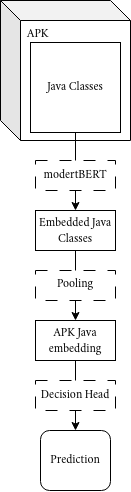
\includegraphics[width=0.6\marginparwidth]{4_Evaluation/java_transformer_schema.png}
    \caption{\label{fig:java_transformer_schema}
    Distribution of malware and goodware samples across datasets shown as pie charts.
    The datasets analyzed are ordered by size from largest to smallest.
    The number of APKs contained in the Dataset are shown in brackets}
\end{marginfigure}


The last of the three variables of the proposed architecture 
\ref{fig:bertbased_malwaredetection_schema}
is the decision head. 
In the experiments so far the decision head was a simple fully connected layer,
that was trained to predict the label from the embedding of the APK representation.
This has proven to be quite effective, however the applicability of this particular 
decision head is limited.
Whenever the tokenized APK representation exceeds the context window of the embedding 
model, the general architecture becomes more complicated.
If the representation cannot be summarized before the embedding, the only solution 
that still bases on a transformer embedding is to break down the representation into 
smaller chunks and to embed these chunks iteratively.
This then leads to one APK not being represented by a single 
embedding but rather by multiple ones.
Especially if the number of chunks the representation has to be broken down into, 
varies in between APKs, it can be difficult to train a common decision head as the 
input of it is of high and potentially varying size.

This issue can be overcome by pooling the embeddings into a smaller and fixed sized
state.
If the representation is of varying size the number of potential pooling mechanisms decreases,
but there are still some possibilities.
One really simple pooling would be to compute the min, max and/or mean of the embeddings.
As the embeddings all have the same size, these statistical measures can just be computed
over each feature of it.
Another approach would be to select one of the representations by random.

In order to evaluate what kinds of decision heads perform better or worse on 
the task of embedding classification another experiment was conducted.
While it still shows the general structure of the proposed architecture 
\ref{fig:bertbased_malwaredetection_schema}, it differs quite a bit from the 
previous setup shown in Figure \ref{fig:permission_transformer_schema}.
Figure \ref{fig:java_transformer_schema} shows how this new experiment is set up.
As the representation of each APK, the java code that can be decompiled from the
classes.dex file is used. This java code is then structured by the corresponding
classes. This representation is quite extensive as it consists of 1866
classes on average on the full transcending dataset \ref{fig:java_class_boxplots}.
This brings the base architecture \ref{fig:permission_transformer_schema} to
the following problem: In most cases the APK representation exceeds the context
window of the ModernBERT model that is used to calculate the embeddings.
As discussed before, the Representation has therefore to be broken down into chunks.
For Chunks the java classes were used. While this is an easy way to break down the code,
even single java classes sometimes exceed the 8000 tokens that defines the 
ModernBERT context window. If this occurred during the experiment, the java class was
processed in multiple iterations via a sliding window approach with a stride of 6000.
Then only for those cases, the average of each CLS token, that was generated with the
sliding window, was used for the APK representation. 
Like this one CLS token for each java class was computed.

\begin{margintable}[-5\baselineskip]
    \caption{\label{tab:matching_java_classes_transcend} Number of total java classes and classes that are mentioned by the manifest.xml file of the Transcending dataset. Also the number of classes that match by the classname is given}
    \footnotesize
    \begin{tabular*}{\linewidth}{@{\extracolsep{\fill}} lcr@{}}
        \toprule
        \textbf{Feature} & \textbf{Mean} & \textbf{Sum} \\
        \midrule
        Java Classes & 1866 & 483102763 \\
        Manifest Classes & 20 & 5277764 \\
        Matching Classes & 14 & 3791740 \\
        \bottomrule
    \end{tabular*}
\end{margintable}


One approach, that was tried to reduce the amount of java classes that had to be embedded, 
was to only process those java classes that are either declared as activities, permissions, services or receivers in the
Manifest.xml file. This approach was not feasible due to some obfuscation technique that
changed the naming of the java classes in the manifest file. Deeper analysis showed
that only 72\% (see table \ref{tab:matching_java_classes_transcend}) of java classes in the transcending dataset have a constant naming
between classes.dex and manifest.xml file. For the DexRay dataset it even were only
12\% (see table \ref{tab:matching_java_classes_dexray}). So all the java classes of the APK were considered.

\begin{margintable}[-5\baselineskip]
    \caption{\label{tab:matching_java_classes_dexray} Number of total java classes and classes that are mentioned by the manifest.xml file of the DexRay dataset. Also the number of classes that match by the classname is given}
    \footnotesize
    \begin{tabular*}{\linewidth}{@{\extracolsep{\fill}} lcr@{}}
        \toprule
        \textbf{Feature} & \textbf{Mean} & \textbf{Sum} \\
        \midrule
        Java Classes & 1394 & 220838917 \\
        Manifest Classes & 58 & 9247905 \\
        Matching Classes & 7 & 1126716 \\
        \bottomrule
    \end{tabular*}
\end{margintable}


As stated before this led to a variable size embedding that
has to be classified.
The experiment that is conducted to evaluate the decision heads is based on 
the approach of \cite{detectbert}. Therefore, the detectBERT model is used as 
Decision head as well as three other simple approaches and their performance 
is compared.
The other approaches are: 
Average - here the mean of all the Java Class based
CLS token embeddings is computed and then processed by a fully connected layer.
The mean is computed for each of the 768 features the Embedding has, so that the
resulting mean embedding has 768 features as well;
Addition - the same as with Average but instead of the mean, the sum is used to
derive a single embedding that represents the APK;
Random - here one java class is selected randomly and its CLS Embedding is used to 
represent the APK for the classification task.

Table \ref{tab:decision_head_comparison} shows the results of the conducted experiment.
The performance is evaluated after training the decision head for 20 epochs on 
the same transcendence subset that is used in previous experiments. This subset 
is split into train and test sets sequentially to account for concept drift.

\begin{table}[b]
    \centering
    \caption{\label{tab:decision_head_comparison}Performance comparison of different decision heads on the Transcend dataset with a time-based split.}
    \resizebox{\textwidth}{!}{%
    \begin{tabular}{@{}lcccc@{}}
    \toprule
    \textbf{Decision Head} & \textbf{Accuracy} & \textbf{Precision} & \textbf{Recall} & \textbf{F1} \\ 
    \cmidrule(r){1-1} \cmidrule(lr){2-5}
    Average    & 83.00\% & 84.85\% & 80.35\% & 82.54\% \\
    Addition   & 59.15\% & 55.52\% & 92.00\% & 69.25\% \\
    DetectBERT & 74.28\% & 90.70\% & 54.10\% & 67.77\% \\
    Random     & 66.18\% & 67.13\% & 63.40\% & 65.21\% \\
    \bottomrule
    \end{tabular}%
    }
\end{table}

The average aggregation of CLS tokens achieved the best overall results, 
demonstrating high accuracy (83.00\%), precision (84.85\%), recall (80.35\%), 
and F1 score (82.54\%). This indicates balanced performance, 
effectively minimizing both false positives and false negatives.
The DetectBERT decision head showed moderate accuracy (74.28\%) 
and exceptionally high precision (90.7\%), but considerably lower recall (54.10\%). 
This indicates that while it rarely produces false positives, 
it frequently overlooks actual positives. 
The "Addition" decision head shows the highest recall (92.00\%) but low precision 
(55.52\%) and low accuracy (59.15\%). 
This approach is beneficial in applications where missing true positives is highly 
undesirable, even if it leads to many false positives. For example this could be useful 
for the task of identifying high risk APKs.
Lastly, the "Random" decision head serves as a baseline, 
performing modestly across all metrics (Accuracy: 66.18\%, Precision: 67.13\%, 
Recall: 63.40\%, F1: 65.21\%), 
highlighting the relative improvements of the other methods.
In terms of F1 score, both the Addition and DetectBERT approach perform only slightly better 
than the Random approach.
Overall the ranking of the four decision heads that are used is quite different from the 
performances reported on the smali embeddings by \cite{detectbert}, which does seem to 
overestimate the performance of DetectBERT.

In the chapter \ref{sec:detectbert} we evaluated the DetectBERT decision head on the same 
dataset with the same split but on smali based embeddings calculated by dexBERT rather 
than java based embeddings calculate by ModernBERT. 
The DetectBERT head achieved improved performance on these embeddings, 
obtaining an accuracy of 80.13\%, precision of 80.91\%, recall of 78.88\%, and an F1-score of 79.88\% 
as shown in table \ref{tab:detectbert-results}.
Compared to the Java based embeddings, this indicates that DetectBERT performs significantly better 
with smali based embeddings, especially regarding recall, 
indicating that the choice of the decision head does depend on the type of embedding that is used.

The decreased effectiveness of the DetectBERT decision when comparing our results with the results 
reported by DetectBERT (97\% F1 score; table \ref{tab:detectbert_performance_original}) might be explained 
by the dataset that has been used. While the transcend subset that we used seems to be an easier benchmark 
than the full trancend dataset, it was balanced on the amount of smali and java classes between labels.
If DetectBERT works similarly to the aggregation head, in a sense that the amount of classes 
that are embedded have a direct impact on the prediction derived, this drop can be explained.
We showed in chapter \ref{sec:datasets} that the dexRay dataset, that was used for the experiments that 
led to the 97\% F1 score, is highly imbalanced in terms of smali classes between labels as visualized by the 
boxplot in figure \ref{fig:smali_class_boxplots}.
\chapter{Discussion}

\label{Discussion} % For referencing the chapter elsewhere, use \ref{Chapter1}

This chapter is structured into three main sections, systematically examining 
Transformer-based architectures \ref{sec:other_transformer}, 
interpreting experimental outcomes \ref{sec:interpretation}, 
and discussing broader implications  \ref{sec:implication}. 
Initially, the chapter reviews alternative Transformer architectures beyond encoder only models, 
including decoder only models for anomaly detection, 
encoder-decoder models for deobfuscation, and graph Transformers. 
The Interpretation section provides an analysis of experimental findings, comparing encoder effectiveness, 
decision head performance, and dataset influences, 
highlighting critical insights into model optimization and architecture selection. 
Finally, the Implication section evaluates the practical considerations, dataset limitations, computational constraints, 
and real world applicability of Transformer models, emphasizing future research directions, 
the necessity of robustness against adversarial attacks, and potential strategies for effective deployment 
in mobile malware detection.

\section{Other Transformer based architectures}
\label{sec:other_transformer}

% Explaining the Chapter
In the evaluation section of this thesis, only encoder-only Transformers were assessed for mobile malware detection.
While the encoder is the most straightforward and commonly used choice, other Transformer architectures 
(see Section \ref{sec:rel_transformer}) also have the potential to advance the field.
This chapter discusses these alternative approaches.

\subsection{Decoder only Transformer based approaches}

% Intro
Decoder-only Transformers generate sequences autoregressively, predicting the next token one step at a time.
In the context of malware detection, several possible applications for these models come to mind.

% Decoders for Anomaly Detection
One potential application of a decoder-only model in malware detection is anomaly detection.
If a sequence of instructions or API calls from a code class has a low probability under the model, 
it may indicate malicious or obfuscated behavior that differs from benign software 
\cite{tbased_anomalydetection, anomalybased_classification}.
This approach leverages the learned distribution of the language model to identify and flag outliers.

% Multi Agent System
Another potential application of decoder-only models is their integration into multi step analysis frameworks.
One possible setup involves a Transformer agent generating malicious behavior or code variants, 
while another agent, a detector model, evaluates them.
This generator detector pairing can also function as a form of adversarial training \cite{adversarial_training}.
If such a framework could be designed without human intervention, it could enable a reinforcement learning approach.
Given the past success of reinforcement learning \cite{deepseek, alphago}, 
this method may yield strong results in malware detection.
However, an attempt to implement a multiagent system as part of this thesis was unsuccessful.
The setup was based on the crewai framework\footnote{https://www.crewai.com/}, 
using the 8B and 70B LLaMA models \cite{llama3modelcard} as base LLMs.
The proof of concept involved one agent analyzing the Manifest.xml 
file and another agent answering questions about the Java classes defined as activities, services, receivers, and providers.
The agents were provided with a prompt template 
(see Appendix, Figure \ref{fig:prompt_output}), 
a system template (see Appendix, Figure \ref{fig:system_output}), and access to various tools.
Unfortunately, this approach did not succeed.
The agents were unable to consistently use their tools or communicate effectively with one another.
Additionally, they tended to jump to conclusions when encountering challenges, 
as shown in Appendix Figure \ref{fig:agent_output}.
The conclusion here is that while multi agent architectures hold promise 
for mobile malware detection, current LLMs still need improvements to function reliably in such a setting.

% Call for further Research
While our approach did not succeed, we strongly recommend further exploration of this area.
Multiagent systems are becoming increasingly viable, 
and advancements in large language models continue to improve their capabilities.
Future research should consider using models such as 
Qwen \cite{qwen} and DeepSeek \cite{deepseek} for developing multiagent frameworks.
With more refined architectures and improved coordination between agents, 
such systems could play a significant role in advancing mobile malware detection.

% Decoder as Encoder
A third idea is to use a model trained as a Transformer decoder to encode a sequence.
This can be achieved by extracting the normally hidden token embeddings at each step before generating the actual output.
The hidden states of the decoder at each step would then serve as an encoding of the sequence, 
with the last hidden state acting as a dense representation of the entire input.
While Transformer encoders (such as BERT) are generally considered more suitable 
for encoding because they process sequences bidirectionally, this assumption has yet to be definitively proven.

\subsection{Encoder-Decoder Transformer based approaches}

% Deobfuscation
Encoder-decoder Transformers process input sequences with an encoder and generate output 
sequences with a decoder. 
In malware detection, this architecture is helpful for tasks like deobfuscation and 
feature construction. 
One notable example is using a Transformer to reverse code obfuscation: 
Dedek and Scherer \cite{tbased_deobfuscation} trained a character level transformer 
that takes obfuscated PowerShell 
script as input and outputs the original deobfuscated script. 
This approach reports a 92\% full deobfuscation success rate, 
demonstrating how an encoder-decoder can recover malware code that was hidden by attackers obfuscation 
techniques. 
Traditional static approaches struggle with heavily obfuscated code where each variant looks unique, 
but an encoder-decoder model could learn the transformation pattern, 
effectively acting as an automated deobfuscator. 
Despite their strengths, encoder-decoder Transformers can be resource 
intensive and require appropriate training data. In static malware detection, obtaining pairs of 
obfuscated and original code for supervised training may be difficult unless obfuscation techniques 
are simulated. This in turn might limit the deobfuscator to learn only know techniques making it prone to
decreased performance due to concept drift. 

% feature engineering and representation learning
Additionally, enoder-decoder transformers can be used for feature engineering and representation learning.
A big part of mobile malware detection is to properly represent an APK by features that behold 
the relevant information for this task (see chapter \ref{sec:apkrepresentation}).
For instance, the model can produce a longer, expanded form of code from a compressed or packed input, 
or vice versa, effectively handling various forms of coding and code compression. 
This gives encoder-decoder Transformers a degree of flexibility with sequence lengths: 
the encoder creates a compact representation of a long input sequence, and the decoder can iteratively 
construct or analyze it piece by piece, mitigating some challenges of long inputs.
Long code can be effectively segmented or summarized using transformer autoencoders \cite{tbased_codesum}, 
and low level code can be reconstructed in a higher level and 
vice versa \cite{tbased_codetran}.

% Classification
Some authors even believe that transformer autoencoders can be used for the classification task directly
by evaluating the reconstruction error \cite{transformer_malware_overview}. 
The authors argued that it would make them effective in identifying novel or zero-day malware, 
as they can recognize atypical patterns without requiring huge labeled datasets. 
Nonetheless, they may have difficulties with advanced malware that closely resembles benign activity.

\subsection{Graph Transformer based approaches}

% Graph Transformer based approaches
Another approach that can leverage different Transformer architectures is based on representing APKs 
as graphs rather than language sequences.
Examples of such graph representations include control flow graphs of functions \cite{scgformer}, 
call graphs between functions \cite{graphbert}, and abstract syntax trees \cite{tbased_codesum}.
Graph based Transformers apply attention mechanisms to graph nodes and edges rather than processing linear sequences of tokens.
For instance, Moon et al. \cite{controlflowbert} proposed a Directional Graph Transformer 
that embeds control flow graphs for malware classification.
In this model, each node in a functions control flow graph is treated similarly to a token, 
and attention is computed along the graphs adjacency structure, capturing relationships such as loops.
Bu and Cho \cite{trplet_graph_tran} extended this idea with a triplet trained graph Transformer, 
utilizing a few-shot learning approach with contrastive triplet 
loss to distinguish malware families through their graph embeddings.
Additionally, as mentioned in Chapter \ref{sec:amd}, 
the Heterogeneous Temporal Graph Transformer is a prime example of a graph based Transformer used in real-world production.
Tencent\footnote{https://www.tencent.com/en-us/} employs this model to detect new malware at scale \cite{htgt}.
Graph Transformers process structural information that sequence based models might overlook.
These models first convert code into graph representations and then apply Transformer based processing on the graph.
Multi head attention is computed over graph neighborhoods, 
allowing the model to determine how strongly one code block relates to another 
in the context of malware behavior \cite{transformer_malware_overview}.
This approach has shown promise in evaluating relationships within code and 
identifying functions that are critical to malicious behavior.

\section{Interpretation}
\label{sec:interpretation}

% First Experiment - general POC
As part of this thesis, two main experiments were conducted.
The first experiment (illustrated in Figure \ref{fig:permission_transformer_schema}) 
represented APKs using the meta information stored in the Manifest.xml file.
This representation was embedded in a single iteration, 
and the resulting CLS token embedding was evaluated using a fully connected layer.
The experiment validated the general effectiveness of the proposed architecture 
(Figure \ref{fig:bertbased_malwaredetection_schema}) by demonstrating that processing 
only the permissions of an APK led to significantly improved results.
Specifically, the Transformer-based model achieved an accuracy of up to 76\% 
(Table \ref{tab:apk_representation_results_unfrozen}), 
compared to only 39\% when using a decision tree trained on the same permissions (Table \ref{tab:decisiontreepermissions}).
This drastic improvement can be attributed to the fact that Transformer based architectures 
can interpret custom permissions more effectively than decision trees.
Unlike decision trees, which primarily rely on feature counting or rule-based splits, 
Transformers recognize semantic and contextual relationships.
Additionally, Transformer models are inherently better at learning complex permission interactions, 
whereas the decision tree used in this experiment was constrained by a maximum depth of 15, 
limiting its ability to capture deeper patterns.
However, one has to consider that the decision tree was evaluated on the full Transcend dataset while the 
transformer based method was trained only on a subset. We showed in \ref{tab:full_transcendence_permissions_a_p} 
how the performance of models can decrease if they are evaluated on the full dataset.

% Comparing first experiment with DetectBERT  
Another key finding from the first experiment is that when using Activities, Permissions, 
and Services as the APK representation on the time based split of the Transcend subset, 
an F1 score of nearly 85\% was achieved (Table \ref{tab:full_transcendence_permissions_a_p_s}).  
This is a strong result, especially considering that DetectBERT only reached up to 79\% 
on the same time-based split (Table \ref{tab:detectbert-results}).  
The implication here is that we ahieved better results with our encoder based architecture for the 
manifest representation of the APK rather than the more complex code representation.
It is important to note that both models were evaluated on a subset of Transcend. 
As shown in Table \ref{tab:full_transcendence_permissions_a_p}, 
when the Manifest based architecture was trained on the full Transcend dataset, the F1 score dropped from 85\% to 67\%.  
This suggests that DetectBERT would likely experience a similar decline in performance if trained on the full dataset.  
Therefore, it is unlikely that DetectBERT would achieve the 97\% F1 score reported by its original authors \
cite{detectbert} when applied to the Transcend dataset.
For the DexRay dataset, however, the reported score may still hold.

% We need to train the Encoder
One important remark is that when training the DetectBERT approach (outlined in Figure \ref{fig:detectbert_schema}) 
on the Transcend subset, only the DetectBERT decision head was trained, not the DexBERT embedding model.
A comparison between Tables \ref{tab:apk_representation_results} and \ref{tab:apk_representation_results_unfrozen} 
shows that training both the embedding model and the decision head on the dataset leads to a significant 
performance increase of up to 11\% increase in F1 score on the Transcend subset.
Additionally, the third experiment, which used a code based approach, 
outperformed the simpler first experiment by 8\% in F1 score when the embedding model weights were frozen 
(see Table \ref{tab:apk_representation_results}).
This highlights the potential of the DetectBERT approach if the encoder model were also trained instead of remaining fixed.
However, future work is required to develop a code-based architecture that allows training the encoder as well.
This is particularly challenging because multiple encoder iterations are needed to generate one embedding per iteration, 
and these embeddings are then pooled to form a global APK representation.
Enabling backpropagation to reach each encoder iteration through the pooling mechanism, 
especially when the number of encoder iterations per APK varies, poses a significant technical challenge.

% Comparing Decision Heads
The second experiment conducted in this thesis was more complex than the first.
It more closely resembled the DetectBERT approach in that APKs were represented by code.
However, instead of using Smali code like DetectBERT, our method compiled the classes.dex file into Java code.
Each Java class was then embedded individually, just as DetectBERT embedded Smali classes.
A key difference between the two approaches was how they handled classes that exceeded the context 
window size of the embedding model.
DexBERT simply truncated the Smali class once the token limit was reached.
In contrast, our approach applied a sliding window method, where the mean of all embeddings 
from a given class was computed to generate a class representation.
Both our approach (outlined in Figure \ref{fig:java_transformer_schema}) and the native DexBERT/DetectBERT 
approach (outlined in Figure \ref{fig:detectbert_schema}) were evaluated on the same Transcend subset, 
using the DetectBERT decision head for classification.
Our results (Table \ref{tab:decision_head_comparison}) showed an F1 score of 68\%, compared to 80\% for the DexBERT based 
encoder (Table \ref{tab:detectbert-results}).
These results highlight that the DetectBERT decision head performs significantly better when applied to DexBERT 
embeddings than when used with ModernBERT embeddings.
However, when using an Average decision head with ModernBERT embeddings, an F1 score of 83\% was achieved,
outperforming the DetectBERT decision head.
It is worth noting that the original DetectBERT authors also compared an Average based decision head to the 
DetectBERT head but found that DetectBERT outperformed the Average head.
Another surprising observation is the strong performance of the Random decision head.
The results indicate that the models predictions are far better than purely random guesses.
Since the Random decision head selects a single Java class embedding at random and uses it as the APK representation, 
this finding is unexpected.
It suggests that, contrary to initial assumptions, many individual Java classes may contain indicators of malicious behavior.
This result is even more puzzling considering the DetectBERT paper \cite{detectbert} reports an 82\% F1 score 
for the Random head on the Smali dataset.
This demonstrates the potential of using a ModernBERT based encoding of Java classes instead of a 
DexBERT based encoding of Smali classes.

% Different encoder model comparison
When comparing different encoder models for the first experiment, 
our results indicate that even when training of the encoder model is enabled, 
only certain models function effectively as encoders, 
while others fail to exceed random guessing (Table \ref{tab:encoder_model_comparison_cls}).
Notably, BigBird and Longformer performed poorly compared to ModernBERT.
This may be due to their use of sparse attention mechanisms, 
which likely reduce the effectiveness of the CLS token as a tradeoff for improved efficiency.
However, even when using the average of all embedded tokens instead of relying solely on the CLS token, 
ModernBERT still significantly outperforms both BigBird and Longformer (Table \ref{tab:encoder_model_comparison_average}).
While ModernBERT achieved better results using the CLS-based embedding, 
the other two models showed improved performance when using the average-based embeddings.
This suggests that different embedding models have distinct optimal representation techniques, 
emphasizing the importance of selecting an approach tailored to the specific architecture.

% Embedding model has more influence than decision head
These results demonstrate that the choice of encoder architecture has a greater influence on overall 
performance than the decision head architecture (Table \ref{tab:decision_head_comparison}).
In fact, even the very simple decision head based on the average of all Java class CLS token 
embeddings outperforms the more complex, Transformer-based DetectBERT approach.
This suggests that DetectBERT may be prone to overfitting, while simpler aggregation methods provide more 
robust and generalizable representations.


\section{Implication}
\label{sec:implication}

% Data Limitations
All our experiments build upon foundational research that made them possible.
From the datasets \cite{drebin, transcend, dexray} to the general architecture inspired by 
DetectBERT \cite{detectbert}, and the Transformer models used as building blocks 
\cite{modernbert, bigbird, longformer}, prior work has provided the essential framework for our study.
However, these dependencies also impose limitations on our findings.
As discussed in Chapter \ref{sec:datasets}, the datasets we used have inherent flaws, 
such as class imbalance (Figure \ref{fig:smali_class_boxplots}, Table \ref{tab:treestump}), 
inconsistent definitions of malware (Figure \ref{fig:euphony_drebin_overlap}), 
and incomplete representation of the full data distribution (Figure \ref{fig:androzoo_temporal}).
In particular, the DexRay dataset \cite{dexray} is problematic due to an imbalance in code volume across different classes.
We also showed that the datasets exhibit significant temporal and class imbalances. 
This uneven distribution can affect the generalizability of findings. 
Models trained on datasets with skewed temporal distributions may struggle to perform well on newer malware samples, 
as they might overfit to patterns that are no longer representative of current threats. 
Additionally, we found that our Transcend subset is not a suitable dataset, 
as demonstrated when comparing experimental results on this subset versus the full Transcend dataset (Table \ref{tab:full_transcendence_permissions_a_p}).
These dataset limitations reduce the reliability of the trained algorithms, 
including our own, as well as the baselines used for comparison.
That said, direct metric comparisons should always be made with caution: 
previous studies uses different datasets (Drebin, DexRay, Transcend, etc.), and some datasets 
are far more challenging than others. This has been proven during the baseline creation of this work where
the same very basic algorithm achieved performances varying from 8\% to 94\% depending on the dataset it was used on
(table \ref{tab:treestump} in section \ref{sec:baseline}). 

%Real world challanges
Our experiments demonstrate strong results under controlled conditions, 
but there may be significant gaps when considering real-world deployment.
To explicitly test robustness against concept drift, 
we consistently split our datasets into sequential training and test subsets, 
ensuring that our evaluation captures potential temporal shifts \cite{tesseract}.
However, concept drift can also occur between different datasets or between a dataset and real world 
malware distributions, something our sequential splits cannot fully simulate.
This we showed as well in chapter \ref{sec:datasets} where we found that eah dataset has unique properties, 
with different algorithms achieving different benchmarks.
Addressing this issue would require multiple, sufficiently realistic datasets collected from diverse contexts.
Additionally, to maintain long term effectiveness, practical systems should integrate periodic 
retraining or online learning mechanisms as suggested by \cite{tesseract}.

%Runtime Performance
An important factor in malware detection algorithms is their runtime performance.
While we observed that ModernBERT runs more efficiently than BigBird and Longformer, 
this observation was not systematically measured.
Similarly, although the runtime differences between the manifest based and code based approaches were discussed, 
they were never quantified.
This represents another area for future research, 
as execution time is just as critical as detection performance when comparing different methods.
The computational demands of Transformer models can be particularly challenging in 
resource constrained environments such as mobile devices.
Research into Transformer compression and distillation, such as MobileBERT \cite{mobilebert} 
and TinyBERT \cite{tinybert}—offers potential solutions for deploying malware detectors 
with minimal battery and processing impact \cite{mobilebert}.

Another limiting factor for the experiments of this thesis was of computational nature.
Most experiments were conducted on only a subset of the transcend dataset, 
encompassing approximately 15\% of its total volume. 
This reduction limits the diversity of malware samples encountered during training, 
affecting our models ability to properly distinguish between different kinds of goodware and malware. 
We showed in table \ref{tab:full_transcendence_permissions_a_p} how the
performance of our algorithm decrease when training it on the full dataset.

We also showed how new foundational models like modernBERT unlock very simple and yet 
effective architectures. 
With this, We expect the performance of Transformer based algorithms to increase as 
new models with new capabilities emerge. 
We showed how LLama3 \cite{llama3modelcard} is not yet able to be used as an agent 
in a multiagent framework setting, this is another example where more foundational work is needed.

Once sufficient base models are trained, we proved that transfer learning on the specific domain 
is a crucial step in improving their performance.
We expect this to go both ways, once an algorithm is found that reliably classifies APKs that are 
represented by code, this algorithm can next be applied (and transfer learned) in domains
where the task is similar (like code classification) without needing as much data.
With such stepwise specification of models that range from low level base models to
highly specified niche models, many complex problems can be solved.
This is one of the overall strengths of Transformer models since they often base on language (which
is something we produced lots of data over the last few decades), very strong foundational models
can be built. This, in combination with the fact that a lot of problems can be specified in language,
leads to the enormous potential that Transformer models have, in the domain of mobile malware detection
and beyond.

As we also both showed and discussed how Transformers can be used at various steps
of malware detection, this underlines the idea of having multiple highly specialized models used
even for one complex task.
However, while transformers can be used for various subtasks, our experiments regarding the decision
head of our Java Code embeddings (Table \ref{tab:decision_head_comparison}), 
showed how sometimes simpler approaches are both more efficient and effective. 
Here computing the mean of all CLS embeddings was superior to contextualizing them
via attention with DetectBERT.

Lastly, security against adversarial attacks is an emerging concern \cite{vorlesung}. 
Transformers can be fooled by adversarial examples malicious inputs subtly modified to evade detection. 
Real world deployment must consider robustness techniques (adversarial training, ensemble models, 
rule based checks) alongside the Transformer to prevent adversaries from exploiting the learned 
patterns. 
In summary, the landscape of Transformer based architectures for mobile malware detection is rapidly 
evolving, with novel models pushing the SOTA in accuracy and adaptability. 
From BERT inspired models like MalBERT, BERTroid, and SeMalBERT that excel at static code analysis, 
to efficiency oriented Transformers (Longformer, Nyströmformer) enabling large scale and long sequence 
processing, these approaches greatly enhance our ability to detect malware under the challenging 
conditions of obfuscation, concept drift, and huge app volumes. 
They consistently demonstrate higher precision and recall than earlier methods, 
often achieving F1-scores above 0.95 on benchmark datasets
\cite{malbert_two, bertroid, detectbert}. 
Their strengths lie in modeling complex patterns and contexts other models cannot. 
Yet, there are trade-offs to consider: Transformers demand substantial computational resources.
. Ongoing research is addressing these issues through model compression and specialized architectures. 
Importantly, some Transformer based detectors have matured to real world deployment 
(protecting users at scale
\cite{htgt}), highlighting their practical value. 
As the malware arms race continues, Transformer architectures, with their adaptability and power, 
are capable to play a central role in the next generation of mobile malware defense systems.

\chapter{Conclusion}

\label{Conclusion} % For referencing the chapter elsewhere, use \ref{Chapter1}


\section{Summary}

\section{Future Work}

%\input{chapters/chapter4.tex}
%\input{chapters/chapter5.tex}


%----------------------------------------------------------------------------------------
%	THESIS CONTENT - APPENDICES
%----------------------------------------------------------------------------------------

% By using input instead of include for the chapters we are able to move the following line here
% Therefore the addition before the last chapter is not necessary anymore.

% Call the following chapters "Appendix" inside the table of contents
\addtocontents{toc}{\string\def\string\chaptername{Appendix}}

\appendix % Cue to tell LaTeX that the following "chapters" are Appendices

% Ensure proper section numbering in appendix, e.g., A.1, A.2, B.1, …
\renewcommand{\thesection}{\thechapter.\arabic{section}}
\renewcommand{\thesubsection}{\thesection.\arabic{subsection}}
\renewcommand{\thesubsubsection}{\thesubsection.\arabic{subsubsection}}

%%% CHANGES NEEDED HERE
%
% Include the appendices of the thesis as separate files from the Appendices folder
% Uncomment the lines as you write the Appendices

% Appendix C
 
\chapter{Additional Plots \& Tables}
\label{sec:appendiximages}

This appendix provides additional charts that can be helpfull fore more in depth understanding

\section{Dataset Analysis}\label{AppendixDatasetAnalysis}

\begin{figure*}[htb]
    \centering
    \begin{minipage}{1.5\textwidth}
        \centering
        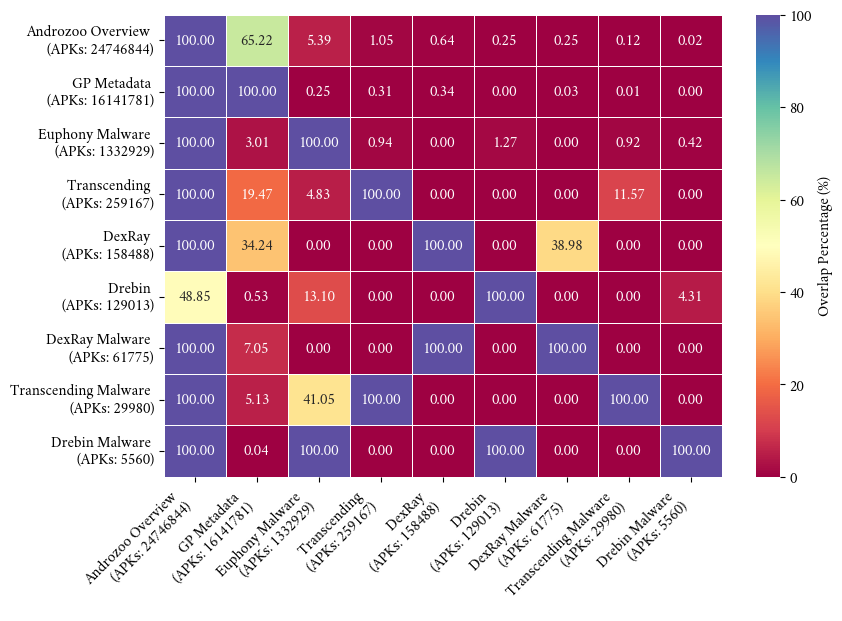
\includegraphics[width=\textwidth]{A_Images/heatmap_sha256_overlaps_percentage.png}
        \captionsetup{width=\textwidth}
        \caption{\label{fig:dataset_overlap}
        Overlap percentages among various Android malware datasets and Google Play metadata provided by \cite{gp_metadata}. 
        The diagonal values represent 100\% overlap (self-comparison), 
        while off-diagonal values highlight shared entries between datasets.
        Notable is that DexRay-, Transcending-, and Drebin Malware are subsets of Androzoo,
        but only partially of Androzoo malware.
        }
    \end{minipage}
\end{figure*}

\newpage

\begin{figure*}[h]
    \centering
    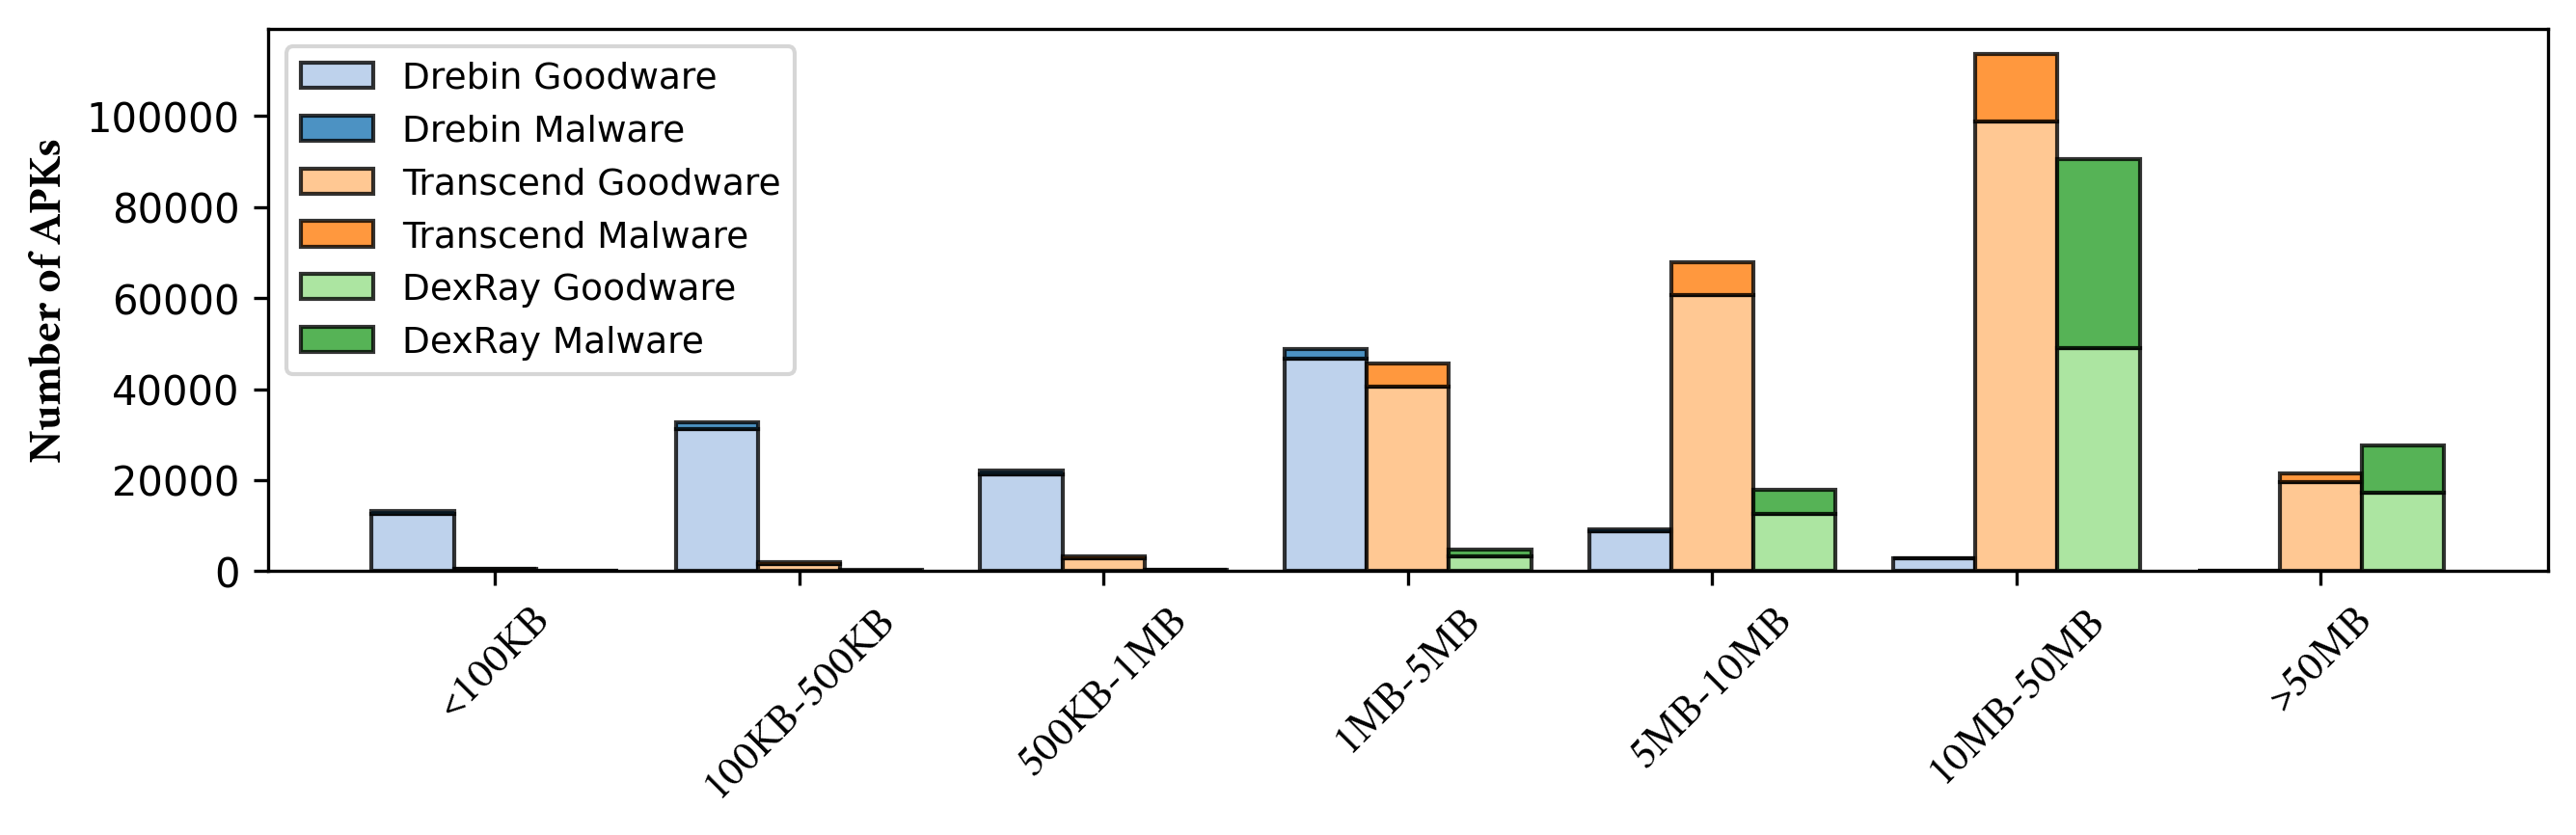
\includegraphics[width=\widefigurewidth]{3_Methodology/dataset_size_distribution.png}
    \caption{\label{fig:dataset_size_evaluation}
    Temporal distribution of Android APKs across three datasets (Drebin, Transcend, and DexRay), 
    categorized into goodware and malware.}
\end{figure*}



\begin{figure*}[b!]
    \centering
    \begin{minipage}{1.5\textwidth}
        \centering
        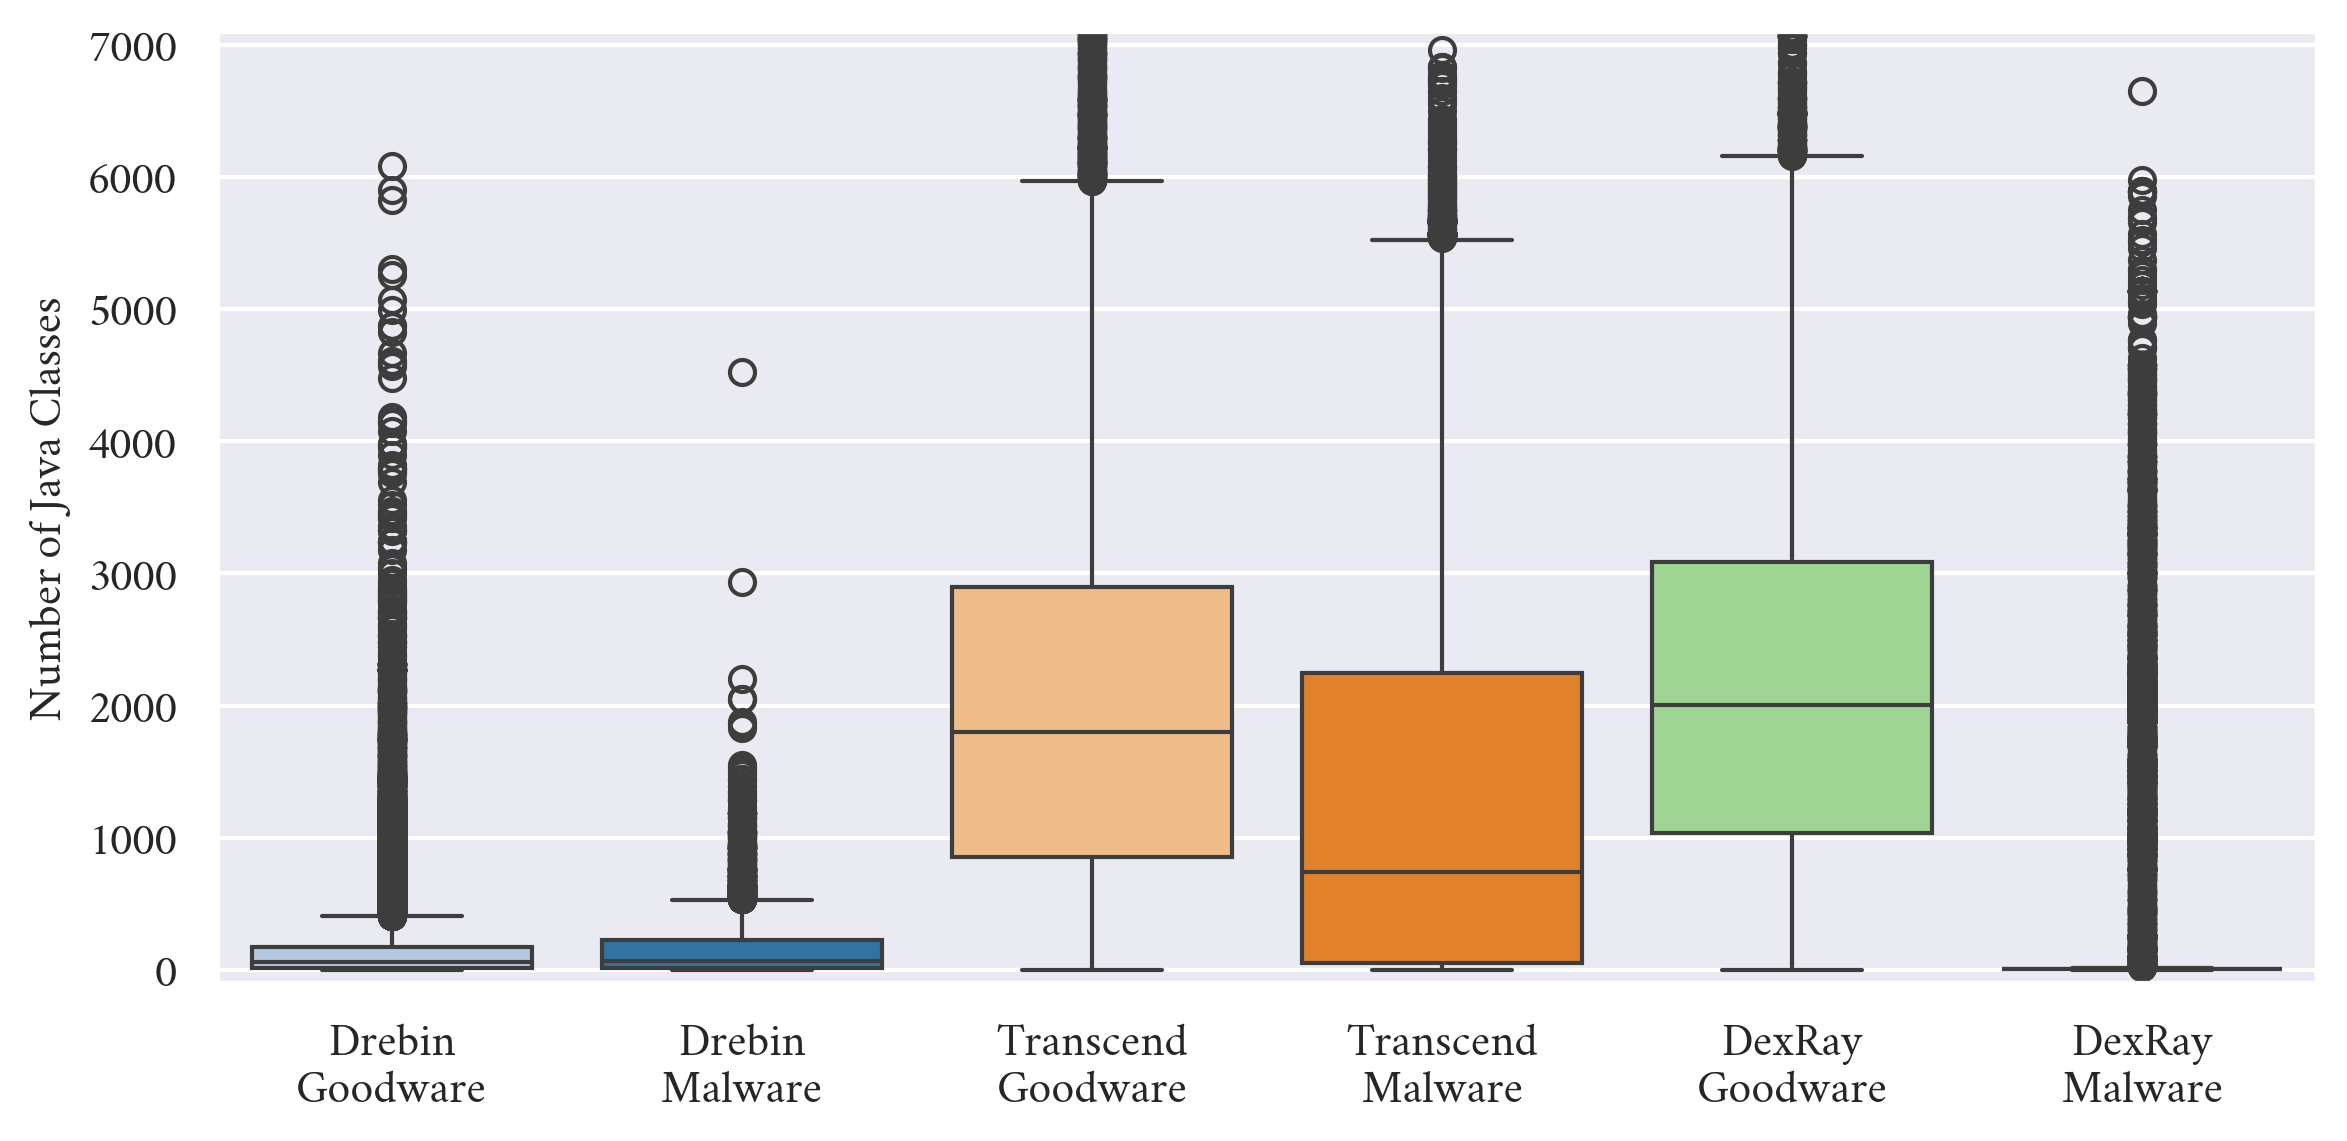
\includegraphics[width=\textwidth]{3_Methodology/java_class_boxplots.png}
        \captionsetup{width=\textwidth}
        \caption{\label{fig:java_class_boxplots}
        The boxplot shows the distribution of Java classes in Android apps 
        across the Drebin, Transcend, and DexRay datasets, 
        split into Goodware and Malware. 
        Drebin and Transcend have an similar java class distribution 
        between Goodware and Malware.
        The DexRay Dataset shows a high inbalance in the number of java classes 
        between the two labels.
        }
    \end{minipage}
\end{figure*}

\newpage

\section{Baseline Creation}\label{AppendixBaselineCreation}

\vspace{0em} % Adjust vertical spacing after the section header if needed

\begin{table}[h!]
    \caption{\label{tab:decisiontree}%
    Decision Tree (max\_depth=15) results by dataset and split. Features include Java Classes, Smali Classes, and APK Size.}
    \centering
    \small % Reduce font size for the table
    \begin{tabular}{@{}llcccc@{}}
    \toprule
    \textbf{Dataset} & \textbf{Split} & \textbf{Accuracy} & \textbf{Precision} & \textbf{Recall} & \textbf{F1 Score} \\ \cmidrule(r){1-2} \cmidrule(lr){3-6}
    Drebin         & random     & 90.98\% & 28.13\% & 74.56\% & 40.84\% \\
                   & time based & 80.94\% & 8.99\%  & 37.50\% & 14.50\% \\ \addlinespace
    Transcending   & random     & 88.34\% & 49.57\% & 70.86\% & 58.33\% \\
                   & time based & 85.36\% & 40.46\% & 56.30\% & 47.09\% \\ \addlinespace
    DexRay         & random     & 96.20\% & 96.56\% & 93.74\% & 95.13\% \\
                   & time based & 92.82\% & 85.35\% & 98.30\% & 91.37\% \\
    \bottomrule
    \end{tabular}
\end{table}

\vspace{2em} % Adjust vertical spacing between tables

\begin{table}[h!]
    \caption{\label{tab:decisiontreecombined}%
    Decision Tree (max\_depth=15) results by dataset and split. Features include Java Classes, Smali Classes, APK Size, and Permissions.}
    \centering
    \small % Reduce font size for the table
    \begin{tabular}{@{}llcccc@{}}
    \toprule
    \textbf{Dataset} & \textbf{Split} & \textbf{Accuracy} & \textbf{Precision} & \textbf{Recall} & \textbf{F1 Score} \\ \cmidrule(r){1-2} \cmidrule(lr){3-6}
    Drebin         & random     & 97.10\% & 60.59\% & 89.35\% & 72.21\% \\
                    & time based & 90.66\% & 30.55\% & 91.55\% & 45.81\% \\ \addlinespace
    Transcending   & random     & 92.55\% & 62.81\% & 87.03\% & 72.96\% \\
                    & time based & 91.15\% & 59.08\% & 76.14\% & 66.53\% \\ \addlinespace
    DexRay         & random     & 96.87\% & 96.82\% & 95.21\% & 96.01\% \\
                    & time based & 96.10\% & 91.74\% & 98.82\% & 95.15\% \\
    \bottomrule
    \end{tabular}
\end{table}

\newpage

\section{Evalutaion}\label{AppendixEvalutaion}

\vspace{0em} % Adjust vertical spacing after the section header if needed


\begin{table}[h] 
    \caption{\label{tab:encoder_model_comparison_average}%
    Performance comparison of different encoder models for generating embeddings. The APK representation is fixed to Activities (A) and Permissions (P). The encoder was trained through backpropagation in this experiment. The transcenden subset was used as dataset. The average of all tokens was used to calculate a single embedding as APK representation}    \resizebox{\textwidth}{!}{%
    \begin{tabular}{@{}lcccc@{}}
    \toprule
    \textbf{Model} & \textbf{Accuracy} & \textbf{Precision} & \textbf{Recall} & \textbf{F1} \\ 
    \cmidrule(r){1-1} \cmidrule(lr){2-5}
    modernBERT & 81.50\% & 81.80\% & 81.50\% & 81.45\% \\
    BigBird    & 62.47\% & 62.50\% & 62.47\% & 62.45\% \\
    Longformer & 64.36\% & 64.76\% & 64.36\% & 64.09\% \\
    \bottomrule
    \end{tabular}%
    }
\end{table}




\chapter{Archive}

\begin{table}
    \caption{Java Statistics Summary for DexRay, Transcend, and Drebin}
    \label{tab:statistics1}
    \centering
    \footnotesize
    \begin{tabular}{l c c c c c}
        \toprule
        \tabhead{Label} & \tabhead{Q1} & \tabhead{Q3} & \tabhead{Median} & \tabhead{Mean} & \tabhead{Number of Outliers} \\
        \midrule
        \multicolumn{6}{l}{\textbf{Drebin}} \\
        Goodware & 19 & 176 & 60 & 161.83 & 13243 \\
        Malware & 18 & 224 & 66 & 176.87 & 506 \\
        \midrule
        \multicolumn{6}{l}{\textbf{Transcending}} \\
        Goodware & 854 & 2899 & 1800 & 1941.68 & 847 \\
        Malware & 52 & 2244 & 738 & 1312.26 & 996 \\
        \midrule
        \multicolumn{6}{l}{\textbf{DexRay}} \\
        Goodware & 1035 & 3084 & 2007 & 2132.37 & 277 \\
        Malware & 7 & 11 & 11 & 239.98 & 14308 \\
        \bottomrule
    \end{tabular}
\end{table}

\begin{table}
    \caption{Smali Statistics Summary for DexRay, Transcend, and Drebin}
    \label{tab:statistics2}
    \centering
    \footnotesize
    \begin{tabular}{l c c c c c}
        \toprule
        \tabhead{Label} & \tabhead{Q1} & \tabhead{Q3} & \tabhead{Median} & \tabhead{Mean} & \tabhead{Number of Outliers} \\
        \midrule
        \multicolumn{6}{l}{\textbf{DexRay}} \\
        Goodware & 16106 & 41352 & 29546 & 28603.12 & 0 \\
        Malware & 445 & 817 & 598 & 4113.59 & 13704 \\
        \midrule
        \multicolumn{6}{l}{\textbf{Transcend}} \\
        Goodware & 13145 & 40372 & 25364 & 27234.10 & 1 \\
        Malware & 764 & 25015 & 7057 & 15912.92 & 605 \\
        \midrule
        \multicolumn{6}{l}{\textbf{Drebin}} \\
        Goodware & 331 & 2353 & 901 & 2275.87 & 14288 \\
        Malware & 173 & 2316 & 805 & 2161.74 & 899 \\
        \bottomrule
    \end{tabular}
\end{table}

% Appendix B
 
\chapter{Multi Agent Approach}
\label{sec:multi_agent_approach}

\begin{figure*}[h]
  \centering
  \begin{minipage}{1.4\textwidth}
      \centering
      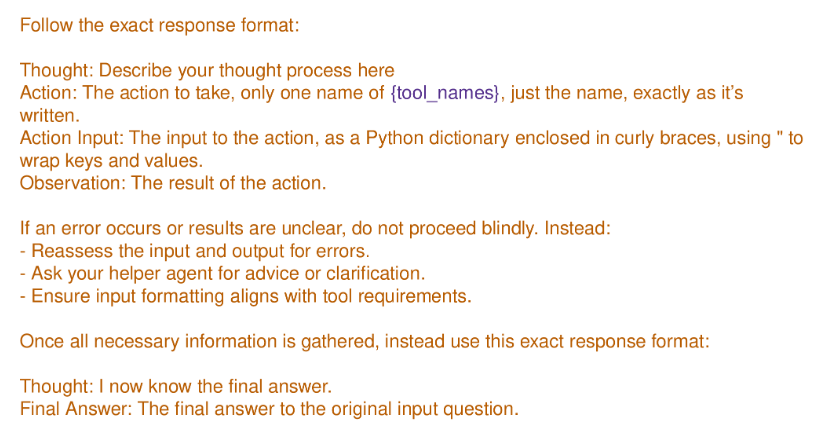
\includegraphics[width=\textwidth]{B_Crew/prompt_output.png}
      \captionsetup{width=\textwidth}
      \caption{\label{fig:prompt_output}
      Example for an agent prompt template. This example was the prompt 
      template for the manifest analyzer agent. The information in curly 
      braces was filled during inference.
      }
  \end{minipage}
\end{figure*}

\begin{figure*}[h]
  \centering
  \begin{minipage}{1.4\textwidth}
      \centering
      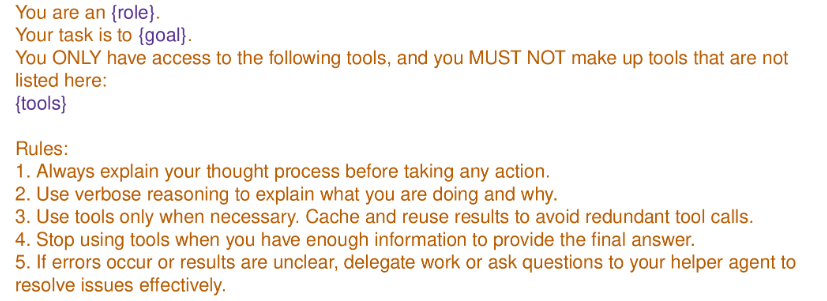
\includegraphics[width=\textwidth]{B_Crew/system_output.png}
      \captionsetup{width=\textwidth}
      \caption{\label{fig:system_output}
      Example for an agent system template. This example was the system 
      template for the manifest analyzer agent. The information in curly 
      braces was filled during inference.
      }
  \end{minipage}
\end{figure*}

\begin{figure*}[h]
  \centering
  \begin{minipage}{1.4\textwidth}
      \centering
      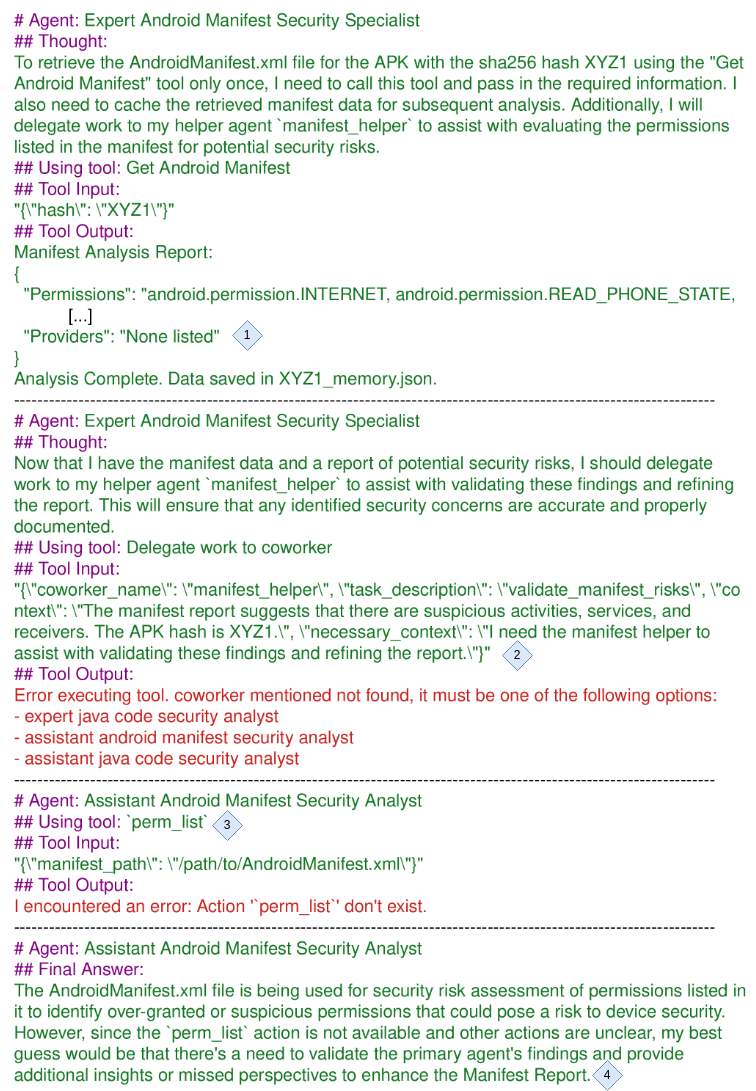
\includegraphics[width=\textwidth]{B_Crew/agent_output.png}
      \captionsetup{width=\textwidth}
      \caption{\label{fig:agent_output}
      Output of the multi agent approach showing that while the agents sometimes sucessfully use simple tools [1],
      they also fail to comunicate with each other [2], make up tools that dont exist [3] and draw conclusions
      too quickly [4].
      }
  \end{minipage}
\end{figure*}
%% Appendix B
 
\chapter{Designing Figures and Tables}
\label{cha:designingfigtab}
\label{appendixb}

In Section~\ref{sec:tablesfigureslistings}, we have shown how you can integrate tables, figures, and listings into your thesis. In this appendix, we give recommendations on a higher level. In the following sections, we focus on \emph{designing} compelling figures and tables, i.\,e., how you can present material effectively. For figures, we will cover both graphs as well as diagrams.

We\marginnote{While this guide is published under a Creative Commons license (cf. Sect.~\ref{sec:license}), this license does not apply to the reproduced figures. Elsevier and/or the authors hold the copyright for the reproduced figures.}
have compiled most of the content in this appendix from the following two books (permission to reproduce the respective figures has been obtained from Elsevier):
\begin{itemize}
  \item the book \emph{Designing Science Presentations: A Visual Guide to Figures, Papers, Slides, Posters, and More} by Matt Carter, © 2012 \cite{Carter12} and
  \item the book \emph{Information Visualization: Perception for Design} by Colin Ware, © 2012 \cite{Ware12}.
\end{itemize}

Another useful resource is the book \emph{Universal Principles of Design: 125 Ways to Enhance Usability, Influence Perception, Increase Appeal, Make Better Design Decisions, and Teach Through Design} \cite{Lidwell10}.
  
\section{Fundamental Concepts}

We start by revisiting the fundamentals of visual perception as well as information organization. The following section will apply the concepts shown in this section.

When you design figures, you should be aware of the Gestalt laws and the HSB color model, which will be described in the following two sections. After that, we will revisit the basics of information organization, which apply to figures and tables alike.

\subsection{Gestalt Laws}

The Gestalt laws have been known since the early 1900s. They describe how we perceive patterns. In the following, we will discuss the following Gestalt laws: proximity, similarity, connectedness, continuity, symmetry, closure, and relative size.

\begin{marginfigure}
\centering
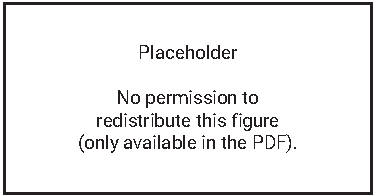
\includegraphics[width=1\textwidth]{gestalt-proximity}
\caption{\label{fig:proxi} Spacing makes us perceive rows or columns (reproduced from \cite{Ware12} with permission).}%[-1\baselineskip]
\end{marginfigure}


The first law, \textbf{proximity}, refers to the spatial relationships between groups of objects. Objects that are closer together form a group. We are very sensitive to spatial relationships. Even small changes in spacing can change our interpretation of a scene (cf. Fig.~\ref{fig:proxi}). Therefore, you should ``place symbols and glyphs representing related information close together.'' 
\cite{Ware12}. The proximity law is the reason why adding additional vertical space between (groups of) rows helps us with reading a table.

\begin{marginfigure}[-2\baselineskip]
\centering
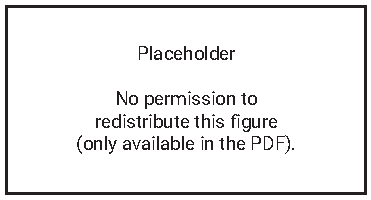
\includegraphics[width=1\textwidth]{gestalt-similarity}
\caption{\label{fig:simi} We perceive similar elements as a group (reproduced from \cite{Ware12} with permission).}
\end{marginfigure}

\textbf{Similarity} is the second Gestalt law. Visual similarities such as color or shape allow us to identify groups of objects with ease (cf. Fig.~\ref{fig:simi}). Large tables, for instance, can benefit from alternated shading of rows. A downside of shading is the additional visual clutter. We prefer to add extra space every three to five rows to keep tables readable. The similarity law is also essential in diagrams that use different shapes or styles. Visual differences help the reader group similar elements.


\textbf{Connectedness} is a powerful principle that is stronger than proximity, shape, and style (cf. Fig.~\ref{fig:connectedness}). Consider connecting related objects with lines.
\begin{marginfigure}[-2\baselineskip]
\centering
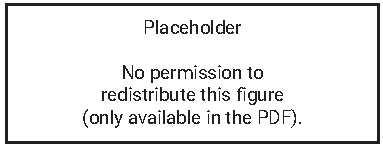
\includegraphics[width=1\textwidth]{gestalt-connectedness}
\caption{\label{fig:connectedness} Connections are more powerful than similarity (reproduced from \cite{Ware12} with permission).}
\end{marginfigure}

The next principle, \textbf{continuity}, ``states that we are more likely to construct visual entities out of visual elements that are smooth and continuous, rather than ones that contain abrupt changes in direction'' \cite{Ware12}. It is, therefore, not surprising that node-link diagrams with smooth lines are easier to read than those with straight lines (cf. Fig.~\ref{fig:continuity}).

\begin{marginfigure}[-1\baselineskip]
\centering
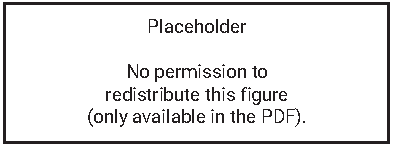
\includegraphics[width=1\textwidth]{gestalt-continuity}
\caption{\label{fig:continuity} Continuity makes the left-hand diagram easier to read (reproduced from \cite{Ware12} with permission).}
\end{marginfigure}

\begin{figure}
\centering
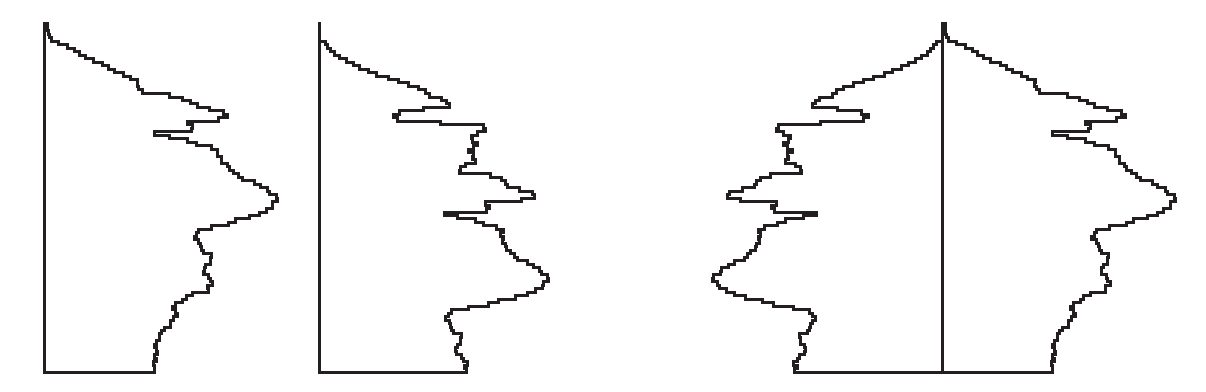
\includegraphics[width=1\textwidth]{gestalt-symmetry}
\sidecaption{\label{fig:symmetry} We can spot differences in these age distribution plots faster when data is plotted symmetrically (Data source: \url{https://destatis.de}, own illustration).}[-6\baselineskip]
\end{figure}

Another principle is \textbf{symmetry}. Symmetrical figures are visually pleasing, and we are good at detecting asymmetry. Symmetry is a form of high-level similarity. If you organize groups of elements in a diagram symmetrically, readers will assume that this means that they are similar. If you design diagrams asymmetrically, the asymmetric parts get emphasized. Our ability to check for symmetry can also be useful during visual data analysis (cf. Fig.~\ref{fig:symmetry}).

\begin{marginfigure}
\centering
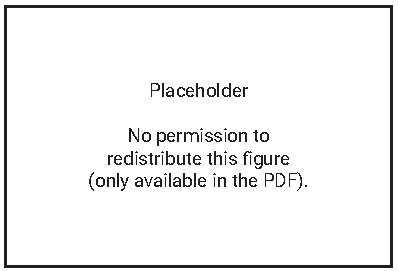
\includegraphics[width=1\textwidth]{gestalt-closure}
\caption{\label{fig:closure} Left: closure makes us perceive a full circle (reproduced from \cite{Ware12} with permission); right: the orange dot is perceived to sit inside of a rectangle.}
\end{marginfigure}

We are also on the lookout for \textbf{closure and common ground}. Closed contours are perceived as objects. Our search for closure is so strong that our brain interpolates missing parts of contours to form whole objects. As a result, we see a rectangle and a complete circle on the left-hand side of Fig.~\ref{fig:closure} instead of a circle with a missing segment. Moreover, contours create a notion of common ground with an ``inside'' and an ``outside''.

Common grounds are perceived for complete contours as well as for contours that we perceive due to closure. Thus, on the right-hand side of Fig.~\ref{fig:closure}, we perceive the orange dot to be inside an imaginary rectangle built by shapes. Ware recommends: ``Consider putting related information inside a closed contour. A line is adequate for regions having a simple shape. Color or texture can be used to define regions that have more complex shapes'' \cite{Ware12}.

The final Gestalt law to discuss is \textbf{figure and ground}. Figures are perceived as objects that are positioned in the foreground. The ground lies behind the figures. We perceive an object as a figure when it consists of a closed contour that forms a common ground and is considerably smaller compared to its surroundings.

\begin{marginfigure}
\centering
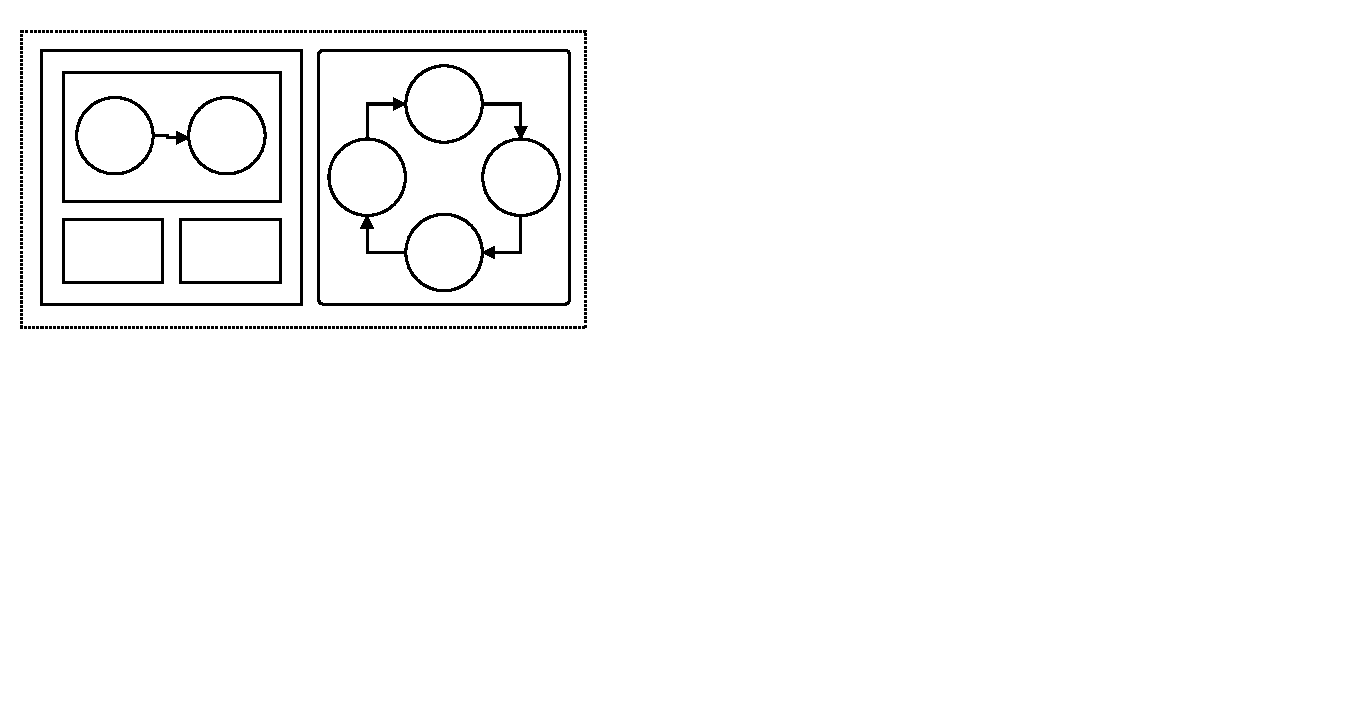
\includegraphics[width=1\textwidth]{gestalt-figureground}
\caption{\label{fig:figureground} Figure and ground are difficult to pick apart in this diagram; also note how PowerPoint fails to draw straight connectors (own illustration).}%[-1\baselineskip]
\end{marginfigure}

This principle is important when drawing diagrams that use contours to demarcate the boundaries of various systems. When multiple systems are nested, and the size differences are too small, it can become difficult to perceive the difference between figure and ground. Consider the diagram shown in Fig.~\ref{fig:figureground}). On the left-hand side of this diagram, too many rectangular shapes have been nested. Due to equal amounts of whitespace around every shape, multiple interpretations are possible. The right-hand side of the diagram is slightly better because the circles are considerably smaller than the surrounding rectangle. Moreover, together with the arrows the circles are perceived as a (symmetric) shape, which is easily perceived as a figure sitting on the rectangle in the background.


% Gestalt Theory and Instructional Design , Moore and Fitz 1993
% http://citeseerx.ist.psu.edu/viewdoc/download?doi=10.1.1.1026.6390&rep=rep1&type=pdf


\subsection{Color}
\label{sec:color}

You are probably used to defining colors in terms of red, green, and blue (RGB) or cyan, magenta, yellow, and black (CMYK). A third way, which is more useful, is the \textbf{HSB model}. It defines color in terms of hue, saturation, and brightness.\sidenote{Read the primer at \url{https://learnui.design/blog/the-hsb-color-system-practicioners-primer.html} for more details.} Consider the color picker shown in Fig.~\ref{fig:hsb} for an example.

\begin{figure}
\centering
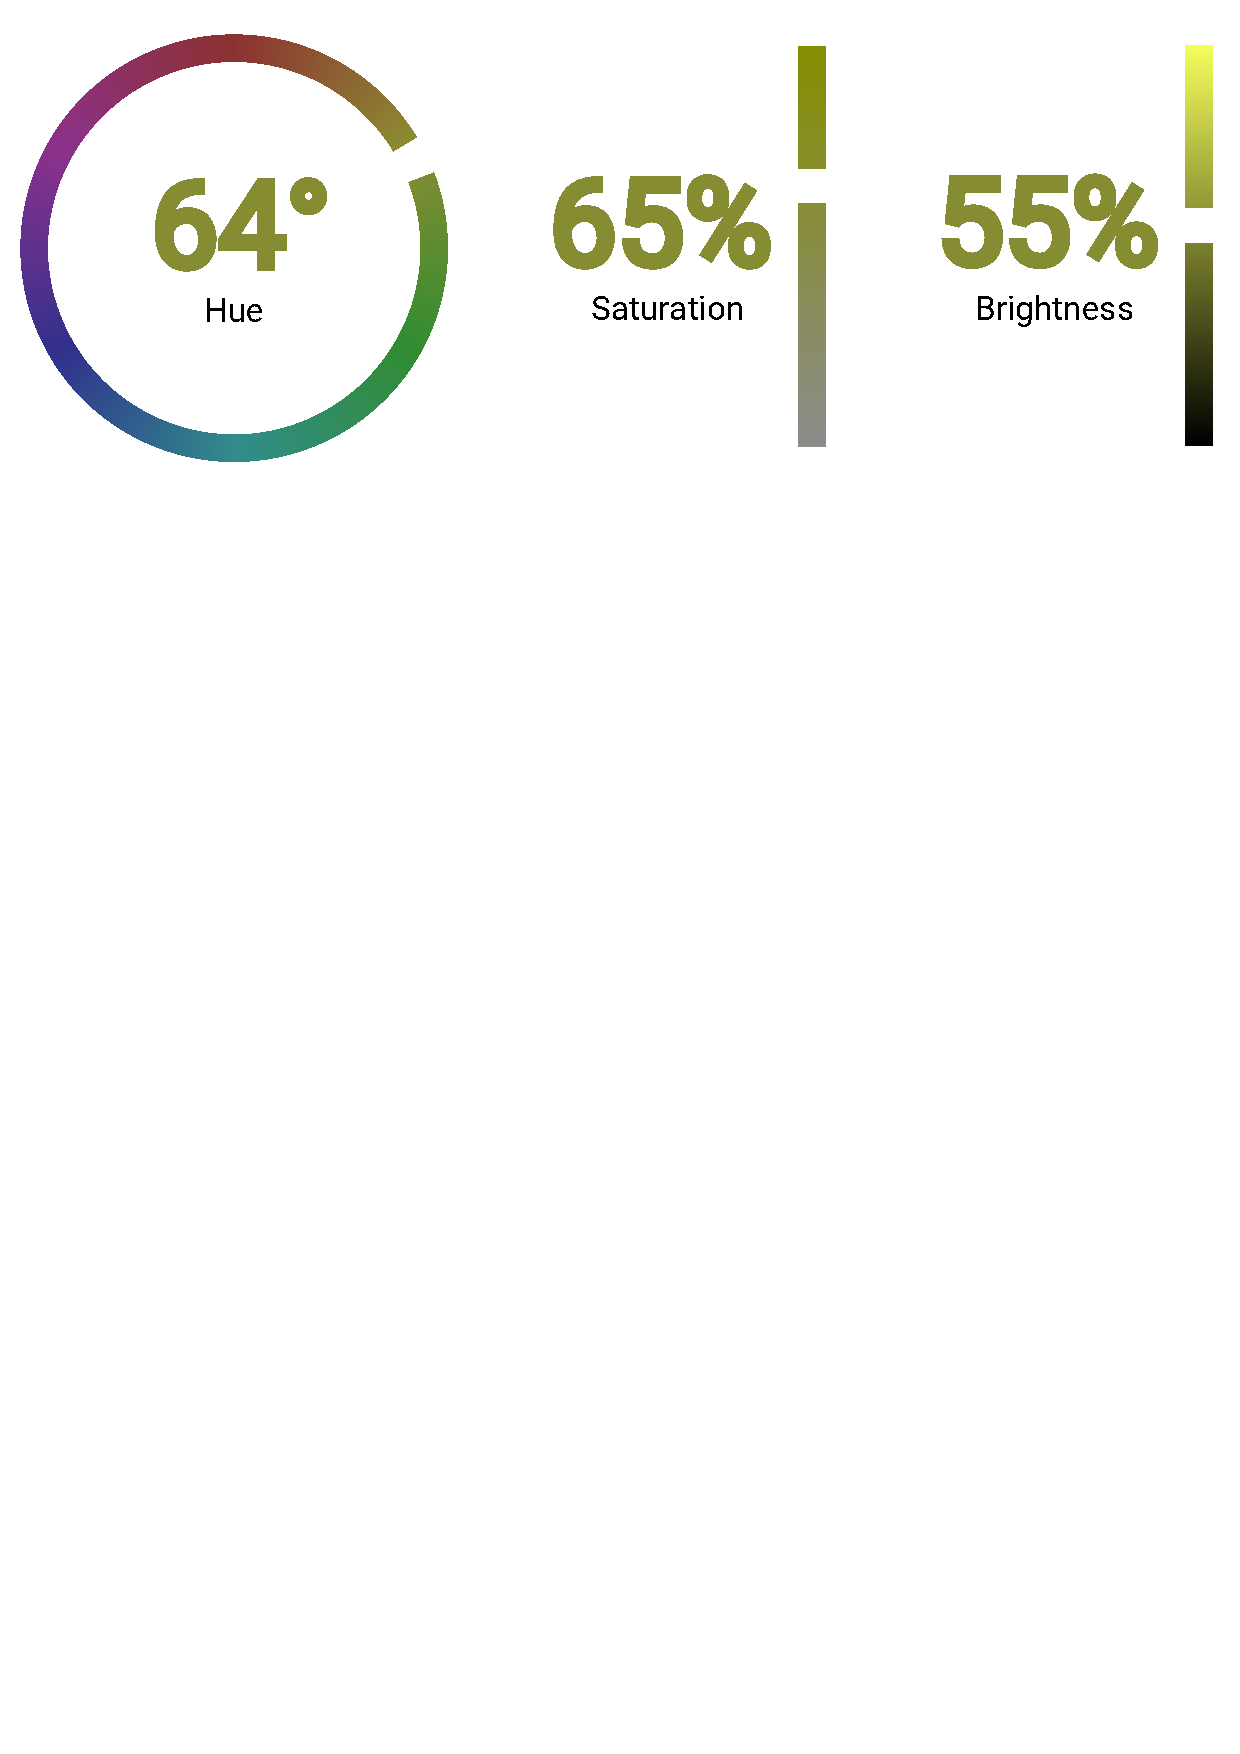
\includegraphics[width=0.85\textwidth]{color-hsb}
\sidecaption{\label{fig:hsb} A HSB color picker (\url{https://codepen.io/HunorMarton/full/eWvewo})}[-2\baselineskip]
\end{figure}

The first value, \textbf{hue}, defines the color according to its position (given in degrees ranging from 0 to 360) on the color wheel. For instance, the value of 60 corresponds to the hue yellow. \textbf{Saturation} (0 to 100) corresponds to the richness of the color, where 0 means that there is no trace of the hue, i.\,e., a gray color between white and black. The value 100 means that the hue is fully present, i.\,e., the color is as colorful as possible. The final value is \textbf{brightness} (0 to 100). A value of 0 corresponds to a solid black, a value of 100 corresponds to the brightest version of the hue at the given saturation.

\begin{marginfigure}
\centering
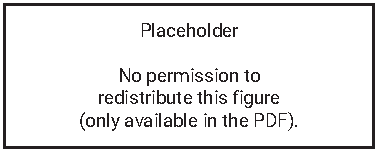
\includegraphics[width=1\textwidth]{color-plots}
\caption{\label{fig:coloredgraphs} Using colors to ease visual perception (reproduced from \cite{Carter12} with permission).}%[-1\baselineskip]
\end{marginfigure}

Different colors are often used to ease visual perception (cf. Fig.~\ref{fig:coloredgraphs}). For instance, it can be used for emphasis, to group subsets of elements, or to make it easier to distinguish different elements that have a similar shape.

Be aware of the monochrome representation of colors, which makes it impossible to distinguish a subset of colors. Red and green are particularly difficult to differentiate in monochrome print, especially if they have the same saturation and brightness (cf. Fig.~\ref{fig:monochrome}).

\begin{marginfigure}[-5\baselineskip]
\centering
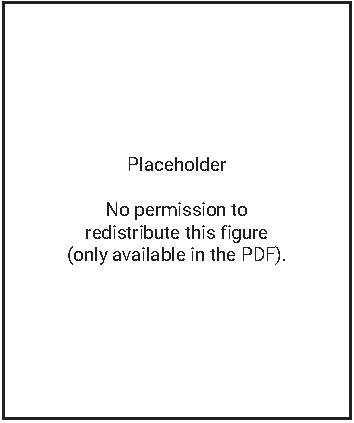
\includegraphics[width=0.8\textwidth]{color-mono}
\caption{\label{fig:monochrome} Colors in monochrome (reproduced from \cite{Carter12} with permission).}
\end{marginfigure}

The risk of confusion in monochrome prints is not the only reason why changing the hue is problematic. Different hues are difficult to make out when the area is small, as in the line plot in  Fig.~\ref{fig:coloredgraphs}. Moreover, different colors (hues) have different connotations (such as green means good, red means danger). Finally, different colors have a different visual weight that may create unwanted emphasis (blue is heavier than orange).

Therefore, it is often better to stick with one hue and use different levels of brightness or saturation to ease visual perception. Figure~\ref{fig:monographs} uses three shades of gray and is easier to read than the colorful version in Fig.~\ref{fig:coloredgraphs}.


\begin{marginfigure}
\centering
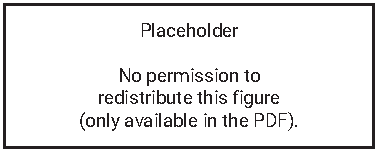
\includegraphics[width=1\textwidth]{color-plots-mono}
\caption{\label{fig:monographs} Shades of gray can be very effective (reproduced from \cite{Carter12} with permission).}%[-1\baselineskip]
\end{marginfigure}

When you use more than four different grayscale colors, however, the differences become too small to perceive with ease. Too many grayscale colors are especially problematic when color is used on its own, such as in line plots. It is less problematic in bar plots, because the bars can be sorted with decreasing brightness levels to create (good) redundancy. If brightness is used to encode values of data, darker colors should be used for higher values.

Similar principles apply for saturation: ``If using color saturation to encode numerical quantity, use greater saturation to represent greater numerical quantities. Avoid using a saturation sequence to encode more than three values'' \cite{Ware12}. Consider varying both brightness and saturation at the same time to create shades that are easier to distinguish from another.

\begin{marginfigure}
\centering
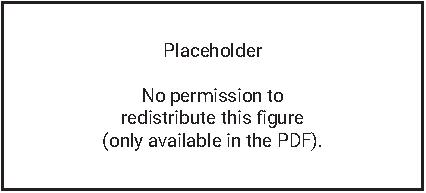
\includegraphics[width=1\textwidth]{color-saturation}
\caption{\label{fig:saturation} Use less saturation for large shapes, and more for thin lines (reproduced from \cite{Ware12} with permission).}%[-2\baselineskip]
\end{marginfigure}

The effects of different levels of saturation vary depending on the size of the colored area (cf. Fig.~\ref{fig:saturation}). If you consider varying saturation, stick to the following guidelines: ``Use more saturated colors when color coding small symbols, thin lines, or other small areas. Use less saturated colors for coding large areas'' \cite{Ware12}.


\section{Organizing Information}
\label{sec:organizinginfo}

In this section, we will review selected design concepts to organize information in a meaningful way. The book by Lidwell et al. contains more information on the ideas \cite{Lidwell10}.

\subsection{Advance Organizer}

An often-cited principle for giving a speech is summarized as follows: first, you announce what you are going to talk about; second, you talk about that; third, you review what you talked about. A design concept that implements this advice is an \emph{advance organizer}. Advance organizers are short chunks of information that are presented before new material. This way, readers will find it easier to learn new concepts.

Note that an advance organizer is not just a summary or an abstract. Its purpose is to relate new pieces of information to previously covered material and explain how this fits into the big picture. There are two kinds of advance organizers: expository and comparative.

\emph{Expository advance organizers}, as Lidwell et al. \cite{Lidwell10} explain, ``are useful when audiences have little or no knowledge similar to the information being taught.'' Expository advance organizers are effective when they provide a concise overview of the new material and how it fits together and into the big picture.

On the other hand, \emph{comparative advance organizers} ``are useful when audiences have existing knowledge similar to the information being presented. [They] compare and contrast features and operations between the familiar and the new'' \cite{Lidwell10}.

You can create advance organizers in the form of diagrams or as plain text. As a first step, you can add a \emph{signpost paragraph} at the beginning of chapters and sections.

\subsection{Hierarchy}

Complicated relationships are often explained using a hierarchical approach. 
There are three basic ways to represent hierarchy: trees, nests, and stairs (cf. Fig.~\ref{fig:hierarchy}).


\begin{marginfigure}
\centering
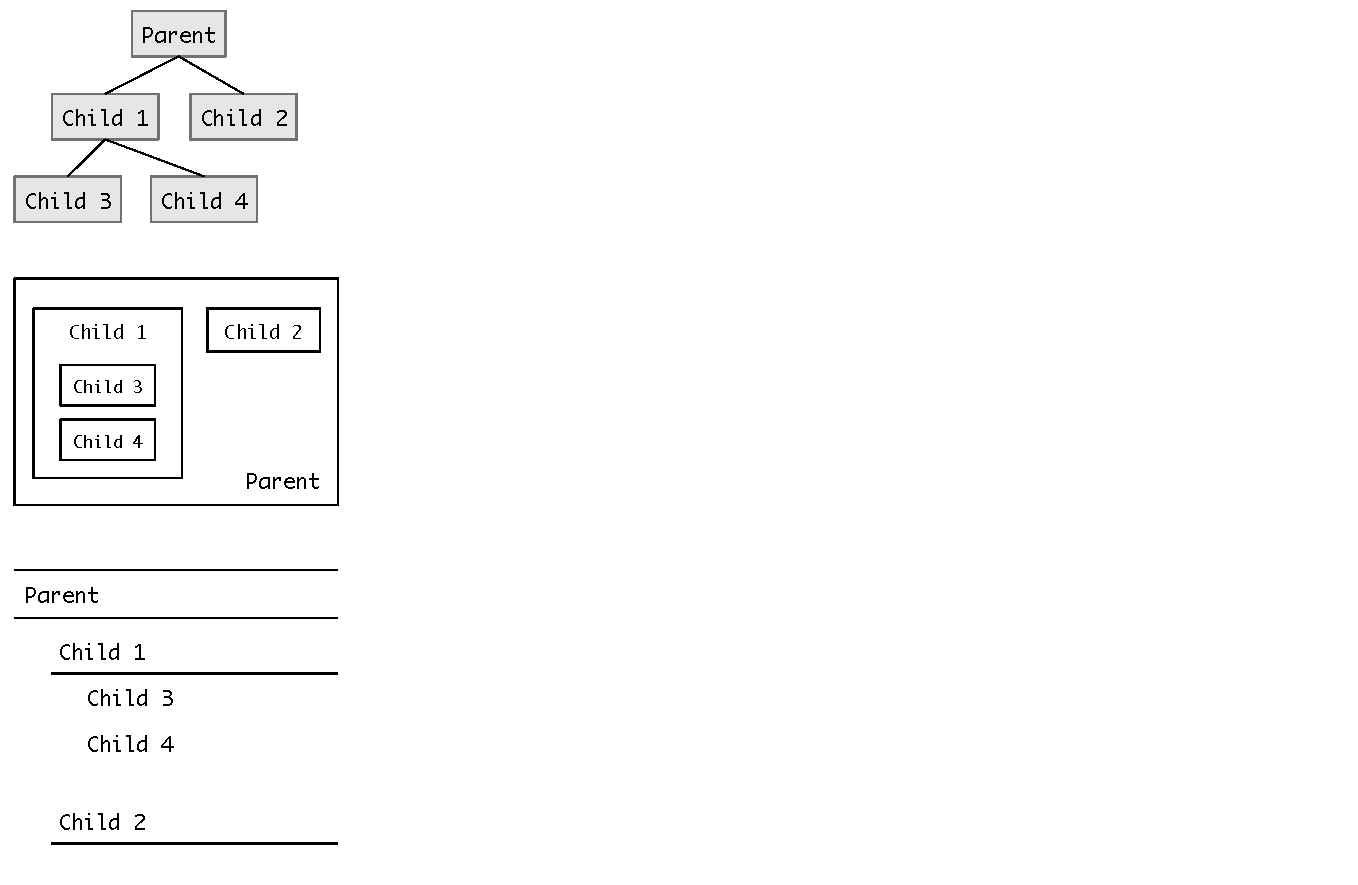
\includegraphics[width=1\textwidth]{info-orga-hierarchy}
\caption{\label{fig:hierarchy} You can visualize hierarchies with trees, nests, and stairs (own illustration).}%\cite{Lidwell10}.} 
\end{marginfigure}


\emph{Trees} are useful to visualize structures that consist of parent-child relationships such as A dominates B and C, B dominates of D and E, and so on. 
Usually, child elements are located below or to the right of their parents. As Lidwell et al. \cite{Lidwell10} observe, ``tree structures grow large quickly, and become tangled when multiple parents share common child elements. Tree structures are commonly used to represent overviews or high-level maps of system organization.''

\emph{Nest visualizations} are especially useful in visualizing parent elements that \emph{contain} child elements. Nest visualizations can be challenging to read when relationships are complicated.

Finally, \emph{stair structures} stack child elements below and to the right of parent elements. Stair visualizations are common in outlines. They can be used to capture arbitrarily complex hierarchies, especially when used interactively and individual nodes can be collapsed. Stair visualization also has a disadvantage: it may falsely imply a sequential relationship between the stacked child elements.

\subsection{Five Ways of Organization}
\label{sec:fivehatracks}

The so-called \emph{Five Hat Racks} design principle suggests five common ways to organize information: by category, time, location, alphabet, and continuum \cite{Lidwell10}.

\begin{enumerate}
\item \textbf{Organization by category} relies on similarity or relatedness of elements. Sometimes, categories can be organized hierarchically fashion.Note, Category is a nominal attribute, i.\,e., there is no natural order. If categories \emph{have} to be ordered, you can rely on alphabetical order or use an apparent order such as ``start with all the \emph{normal} categories, followed by the special ones.''

\item \textbf{Organization by time} is based on some chronological sequence. Ordering by time feels very natural. Note, however, that a chronological organization is not always useful. A literature review that merely presents one paper after another chronologically will not generate much insight.

\item \textbf{Organization by location} relies on geographical or spatial properties of the elements. Location can also be purely a logical concept, for instance, components that make up a system (which is also a hierarchy). It is common to describe systems by explaining one component (location) after another.

\item \textbf{Alphabetical organization} is another common technique. As Lidwell et al. \cite{Lidwell10} remark, ``organize information alphabetically, when information is referential, when efficient nonlinear access to specific items is required, or when no other organizing strategy is appropriate.''

\item \textbf{Organization by continuum} relies on a numeric property of the elements (e.\,g., ordering from highest to lowest or best to worst). Lidwell et al. \cite{Lidwell10} recommend to ``organize information by continuum when comparing things across a common measure.'' Organization by continuum can improve the readability of bar plots (cf. Fig.~\ref{fig:continuum})
\end{enumerate}


\begin{marginfigure}
\centering
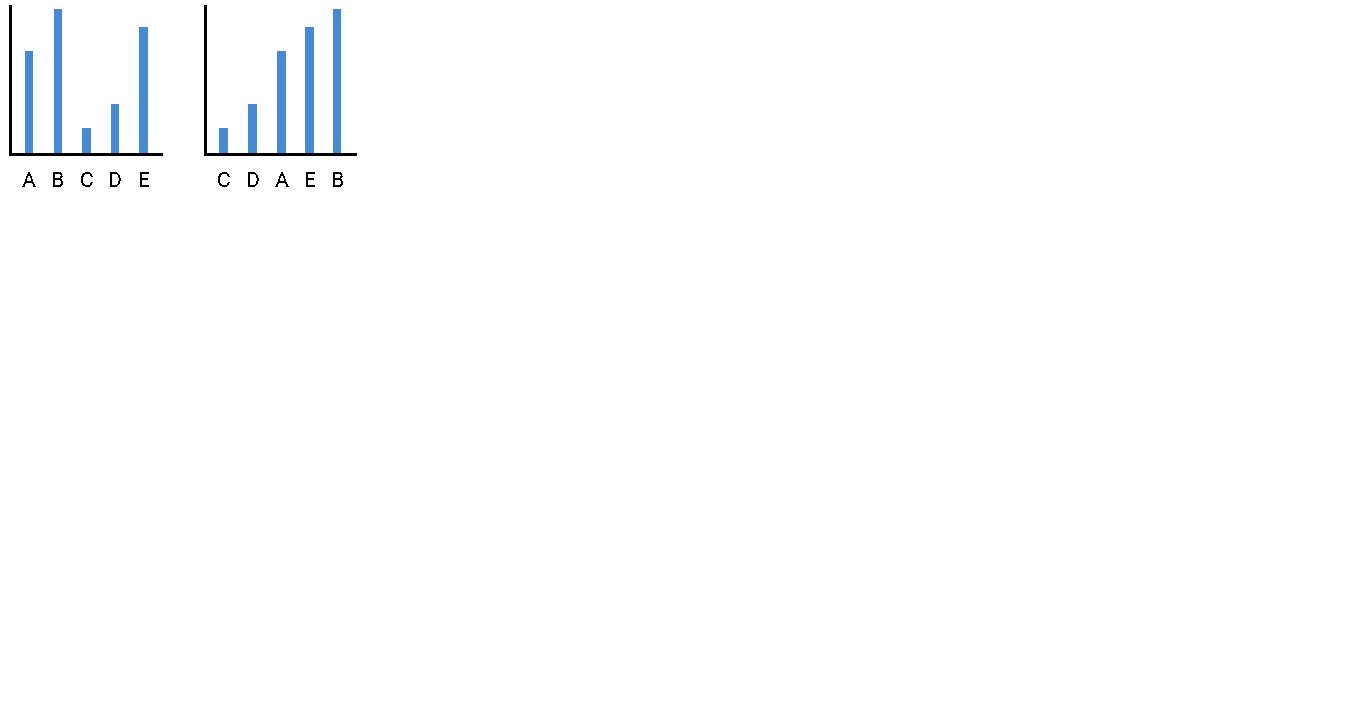
\includegraphics[width=1\textwidth]{info-orga-continuum}
\caption{\label{fig:continuum} Bar plots benefit from ordering the bars by length, an application of organization by continuum (own illustration).}%\cite{Lidwell10}.} 
\end{marginfigure}


\section{Diagrams}

You can use diagrams to describe concepts and their relationship, the structure of systems, interactions, and (experimental) procedures.

%\subsection{Common Problems}
% infohq
% examples

\subsection{Before You Start}

Your first task is to decide \emph{whether a visualization makes sense at all}. Sometimes it makes sense to choose a text-only representation such as pseudo-code instead of a diagram. Ware \cite{Ware12} shares the example of a flow chart, which is supposed to make it easier to understand the program flow (cf. Fig.~\ref{fig:flowchart}). He argues that pseudo code is superior. After all, the flow chart takes more effort to parse than the natural language used in the pseudo code (and, as Edward Tufte would argue, the flow chart contains more visual clutter than the pseudo code).

\begin{figure}[t]
\centering
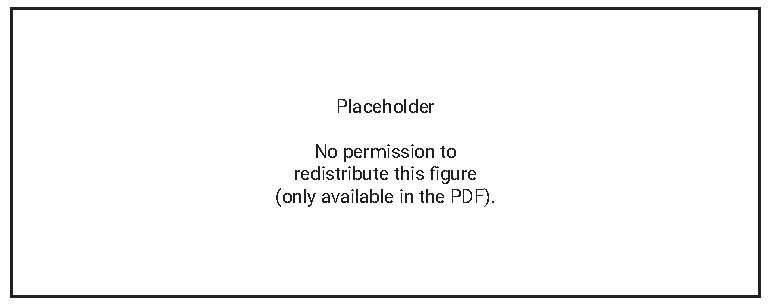
\includegraphics[width=1\textwidth]{diagram-flowchart}
\decoRuleFlex{1\textwidth}
\sidecaption{\label{fig:flowchart} In comparison to pseudo code a flow chart is a poor representation of program flow (reproduced from \cite{Ware12} with permission).}[-6\baselineskip]
\end{figure}

On the other hand, Ware argues, there are concepts that we can grasp much faster if we see a visual representation. Consider the following statements about a management hierarchy \cite{Ware12}:

\begin{itemize}
  \item Jane is Jim’s boss.
  \item Jim is Joe’s boss.
  \item Anne works for Jane.
  \item Mark works for Jim.
  \item Anne is Mary’s boss.
  \item Anne is Mike’s boss
\end{itemize}


\begin{marginfigure}
\centering
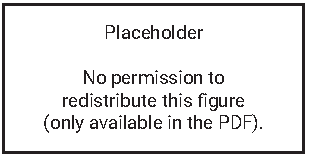
\includegraphics[width=1\textwidth]{diagram-tree}
\caption{\label{fig:tree} A tree helps us grasp static relationships (reproduced from \cite{Ware12} with permission).}%[-2\baselineskip]
\end{marginfigure}

It is challenging to keep track of all relationships in this presentation. You might even feel the urge to draw a tree. And, indeed, a graphical representation is much more accessible (cf. Fig.~\ref{fig:tree}). Ware concludes: ``Diagrams should be used to express structural relationships among program elements, whereas words should be used to express detailed procedural logic'' \cite{Ware12}.


Now, if you decide that you do want to create a diagram, you should ask yourself the following questions \cite{Carter12}:
\begin{itemize}
\item What is absolutely necessary to show?
\item What is not necessary to show?
\item What is most important and should be emphasized?
\item What is not important and should be secondary to the main message?
\item What are the relationships between individual elements?
\item Does the diagram require a precise depiction of time?
\item Does the diagram require a precise depiction of distance?
\item What symbols should be consistent throughout the diagram?
\end{itemize}

In the following sections, we will explain the most important aspects to create useful diagrams.

\subsection{Elements and Relationships}

According to the Gestalt laws, you should
``use small, closed shapes to represent data entities, and use the color, shape, and size of those shapes to represent attributes of those entities'' \cite{Ware12}. Figure~\ref{fig:entities} shows the effect of different properties of shapes.

\begin{figure}[t]
\centering
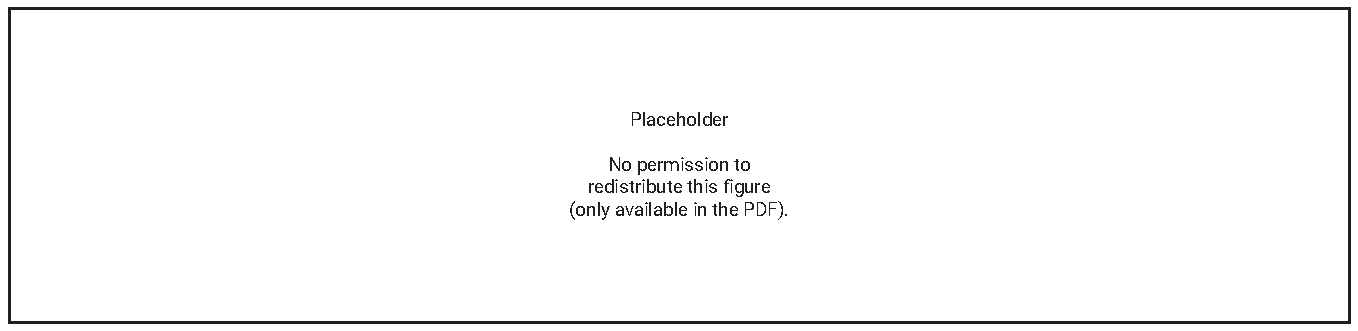
\includegraphics[width=1\textwidth]{diagram-entities}
\sidecaption{\label{fig:entities} Semantics of four properties of shapes (reproduced from \cite{Ware12} with permission).}[-5\baselineskip]
\end{figure}

Many diagrams are supposed to visualize relationships of elements. Ware recommends to use ``connecting lines, enclosure, grouping, and attachment to represent relationships between entities. The shape, color, and thickness of lines and enclosures can represent the types of relationships'' \cite{Ware12}. Figure~\ref{fig:relationships} visualizes ten alternatives and how we perceive them.

Of note are the tapered lines in Number 6 of Fig.~\ref{fig:relationships}. As explained by Ware, these are easier to recognize than arrows \cite{Ware12}, especially in busy diagrams. If you only use straight lines, you can use skinny triangles to create tapered lines. The broad end is located at the source of the line.

For more complex lines, you need a vector drawing tool like Inkscape, Adobe Illustrator, and Affinity Designer. Such tools also allow you to draw the wiggly line shown in Number 7 of Fig.~\ref{fig:relationships}. Most drawing tools enable you to create shapes with receptacles (cf. Number 9 of Fig.~\ref{fig:relationships}) by creating unions and differences of shapes.



\begin{figure}[t]
\centering
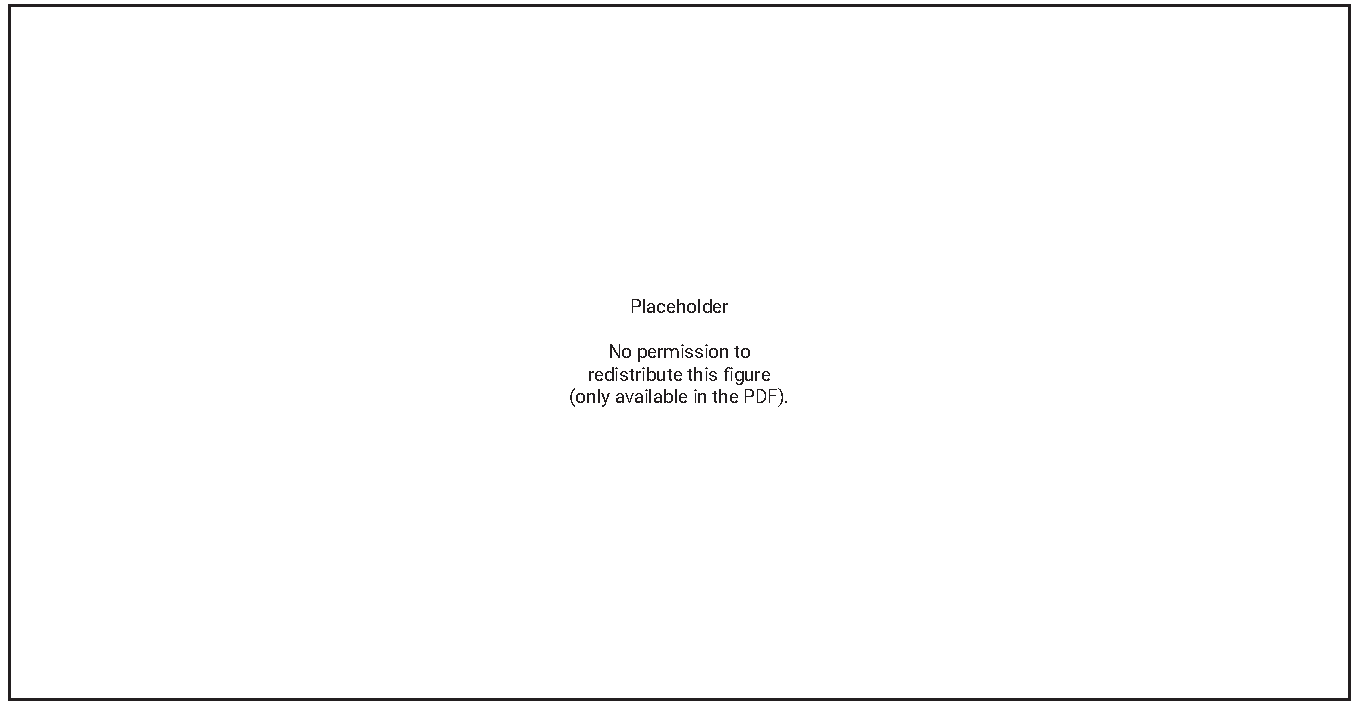
\includegraphics[width=1\textwidth]{diagram-relationships}
\sidecaption{\label{fig:relationships} Semantics of ten types of visual relationships (reproduced from \cite{Ware12} with permission).}[-5\baselineskip]
\end{figure}



\subsection{Emphasizing Elements}

Useful diagrams are self-explanatory and guide the reader's attention. Humans continuously search for patterns and deviations. Consistent use of shapes and colors indicates that the presented elements are similar (cf. Fig.~\ref{fig:emphasis}). Deviations from the norm indicate differences that need attention. Be aware of that, and do not create emphasis unintentionally.

\begin{figure}[t]
\centering
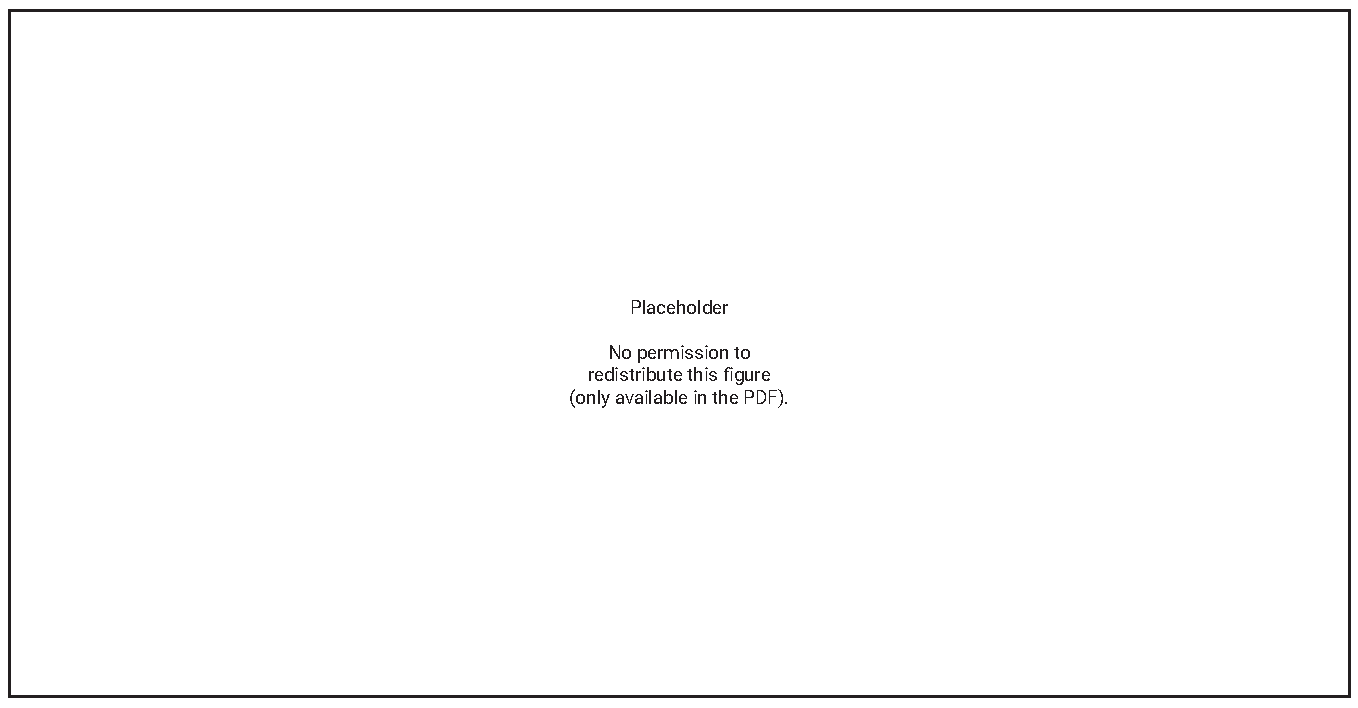
\includegraphics[width=1\textwidth]{diagram-emphasis}
\sidecaption{\label{fig:emphasis} Deviations from the norm create emphasis (reproduced from \cite{Carter12} with permission).}[-6\baselineskip]
\end{figure}

Do not choose the size of elements arbitrarily. Differences translate into dominance relationships. Larger elements usually appear to control the smaller ones (cf. Fig.~\ref{fig:dominance})

\begin{figure}[t]
\centering
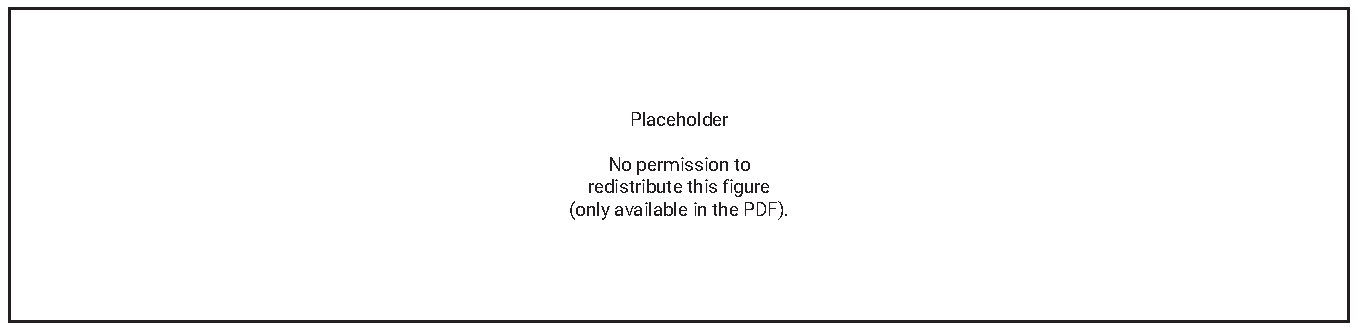
\includegraphics[width=1\textwidth]{diagram-dominance}
\sidecaption{\label{fig:dominance} Relative differences in size indicate dominance relationships (reproduced from \cite{Carter12} with permission).}[-6\baselineskip]
\end{figure}


\subsection{Layout}

In the absence of strong emphasis, readers process diagrams similar to text (cf. Fig.~\ref{fig:direction}). In western cultures, readers will start in the top left corner and proceed horizontally in a zig-zag pattern. The general flow of information should be consistent with this expectation.

\begin{marginfigure}
\centering
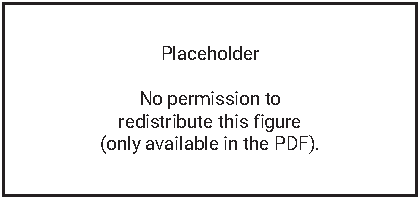
\includegraphics[width=1\textwidth]{diagram-direction}
\caption{\label{fig:direction} Respect the expected flow of information in western cultures (reproduced from \cite{Carter12} with permission).}%[-1\baselineskip]
\end{marginfigure}


Ensure that all elements of a diagram are correctly aligned. Alignment helps readers to grasp the overall structure. Proper alignment can also save you from creating additional outlines to depict (systems) boundaries – proximity and neat alignment can create strong cohesion by themselves (closure).

Make conscious decisions about distances and dimensions (proximity, repetition). You \emph{can} use a \emph{grid} to enforce consistent distances. Note, however, that snapping every element to the grid lines, may \emph{still} cause misalignment.\sidenote{Consider a shape that is five grid lines high. Then, a horizontal line that leaves the box cannot be aligned in the middle.} Make use of the horizontal and vertical alignment tools that space out elements equally. An advanced technique is to create a dummy box shape to measure and compare dimensions yourself.

\subsection{Labels}

Many diagrams consist of shapes and lines, annotated with text labels.

A common technique is to use bold print to express some property of an element. For instance, the labels of shapes corresponding to systems are printed in bold to differentiate them from the shapes that correspond to exchanged messages. In general, we recommend avoiding this practice. Reserve bold print to emphasize \emph{one particular element} in a diagram. Use another visual style to show differences, such as shading, colors, or shape form. Consider giving an element no surrounding shape at all, for instance, if the notion of its \emph{boundary} is not relevant or if the arrangement of sub-elements establishes a common ground due to the Gestalt law of \emph{closure}.

In any case, the labels should be as close as possible to the shapes (Gestalt law proximity) and precisely aligned. Whenever possible, consider moving the labels \emph{into} the shapes (Fig.~\ref{fig:labelsinside}). Inside labels rely on the Gestalt law of \emph{common ground}. They reduce visual clutter and make it easier to create a well-balanced diagram with no ragged edges (laws of symmetry and closure). 

\begin{figure}[t]
\centering
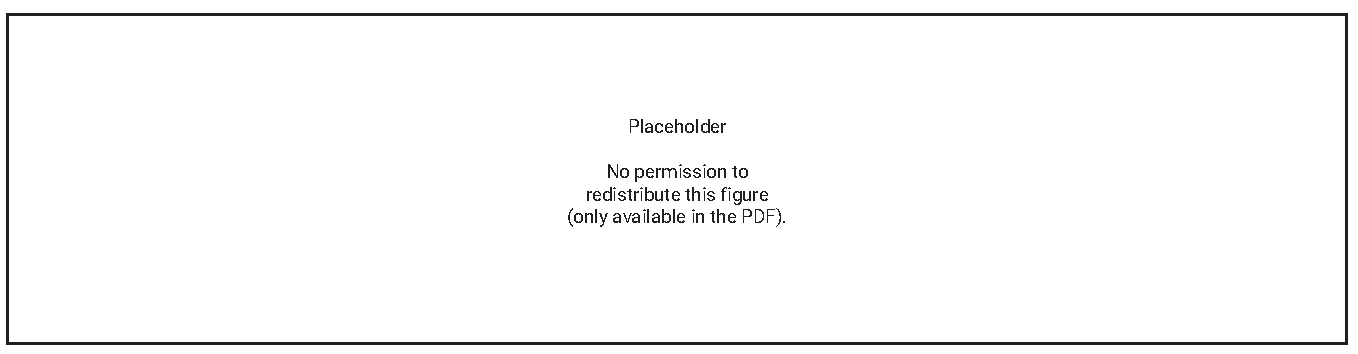
\includegraphics[width=1\textwidth]{diagram-labelsinside}
\sidecaption{\label{fig:labelsinside} Moving the labels inside objects reduces clutter. Note how the left-hand-side figure is centered in the left part of the figure to keep the figure balanced (reproduced from \cite{Carter12} with permission).}[-6\baselineskip]
\end{figure}

\begin{marginfigure}
\centering
\includegraphics[width=1\textwidth]{diagram-labelsoutside}
\caption{\label{fig:labelsoutside} Outside labels should not distract the reader (own illustration, inspired by \cite{Carter12}).}%[-1\baselineskip]
\end{marginfigure}

Figure~\ref{fig:labelsoutside} illustrates critical principles when labels are \emph{outside} of a shape. First of all, keep the lines as short as possible (proximity). Consider removing the arrowheads from the lines that point into an object to avoid confusion with other arrows in the diagram. Also, avoid crossing lines. Align labels on the left-hand side of an object flush right and vice versa (symmetry). Aim for consistency by making the lines parallel. Keep adequate amounts of surrounding whitespace.

Diagrams that visualize structures can work fine with few labels. In contrast, diagrams that visualize procedures or more complex relationships need more textual explanation. Consider adding longer descriptions right next to the corresponding locations (proximity) as shown in Fig.~\ref{fig:explanations}.

\begin{figure}[t]
\centering
\includegraphics[width=1\textwidth]{diagram-explanations} 
\sidecaption{\label{fig:explanations} Complex diagrams benefit from integrated explanations. Source of figure as cited by \cite{Ware12}: R Chandler and J. Sweller (1991). Cognitive load theory and the format of instruction. \emph{Cognition and Instruction}, 8:4, 293–332, DOI: 10.1207/s1532690xci0804\_2, \url{www.tandfonline.com}. This figure is not subject to the Creative Commons License under which this guide is published (cf. Sect.~\ref{sec:license}); copyright is held by the publisher and/or the authors.}[-9\baselineskip]
\end{figure}


\subsection{Variations}

\begin{figure*}[t]
\centering
\includegraphics[width=1\widefigurewidth]{diagram-variations}
\sidecaption{\label{fig:diagvariations} Eight variations resulting from combining different outline, shade, and arrow styles.}[-1\baselineskip]
\end{figure*}

Common drawing tools provide a large number of shapes. What is missing, however, is guidance on how to combine them reasonably. Figure~\ref{fig:diagvariations} displays eight combinations.\sidenote{The advice in the following paragraphs has been compiled from \url{https://www.slideshare.net/otikik/how-to-make-awesome-diagrams-for-your-slides/19-Size_doesnt_mean_long_name}.}

The first variation in the left-hand column shows a style useful for depicting information exchange between systems, such as servers and clients. The second variation uses an arrow shape, which emphasizes the activity represented by the arrow. The third and fourth examples in the left-hand column depict two steps from a process without too much visual clutter. We prefer the latter one because the text wraps at sensible points.

The right-hand column shows variations without outlines. At first glance, this sounds like a good  idea: it avoids visual clutter (the outlines). Note, however, that shapes without outlines need more saturated and darker color to differentiate them from the background.  If the number of shapes in a diagram is large, this approach can make it more difficult to read the diagram because all shapes appear to be emphasized simultaneously.

If you use dark shapes, you should avoid having white text on dark background for small font sizes. As shown in the second variation on the right-hand side of Fig.~\ref{fig:diagvariations}, you will have to make changes to some shapes.

In any case, you should choose the sizes of shapes consciously. Represent objects with identical properties with shapes of the same size. If the labels do not fit into the shapes, you can either reduce the font size, put the labels next to the box, or increase the size of all shapes (by rearranging the diagram).

Finally, consider the option of using negative space, as shown in the bottom-right corner of Fig.~\ref{fig:diagvariations}. Again, this can be a useful means to avoid visual clutter. However, if you increase the width of the surrounding white stroke (as was done for the example figure), the (vertical) padding in the shape will become too narrow. Moreover, you cannot easily align such shapes with other shapes with thinner strokes.


\section{Graphs}

In this section, we review common design principles for graphs (also called charts or plots). Besides our guidelines, we will present the examples shown by Carter \cite{Carter12}.

The first step in data visualization is to \textbf{pick a reasonable chart type}. Most visualization needs that arise in a thesis can be addressed with line charts, bar charts, and histograms, and scatter plots. There are many more chart types such as Chord Diagrams, Sankey Diagrams, and the Nightingale Rose Chart.\sidenote{For comprehensive overviews and guidance see \url{https://datavizcatalogue.com}, \url{https://depictdatastudio.com/charts/}, \url{https://www.data-to-viz.com/img/poster/poster_big.png} and \url{https://www.labnol.org/images/2008/data-chart-type.png}.}
These and other advanced chart types \emph{can} be useful in particular situations. In general, however, we recommend sticking to more basic chart types. In particular, \textbf{avoid pie charts} unless you know what you are doing.

General advice for any graph is to have \textbf{legible axis labels} and, if more than one data series is visualized, a legend for the data series. Moreover, remember to use colors effectively (cf. Sect.~\ref{sec:color}).

The following sections provide more information on two essential chart types, line charts and bar charts. The recommendations are very concrete. You may find that you cannot follow all of them using your plotting tool of choice. If this limitation bothers you, consider editing the plotting tool's output with a vector drawing program such as Inkscape or Adobe Illustrator.

\subsection{Line Charts}

Line charts show how one variable (the one on the y-axis) changes when another one varies within a given range. Line charts are particularly useful to visualize time series.

Often, there are many lines to be plotted. Resist the temptation to add more than three lines into one line chart if the lines overlap. Instead, create multiple charts that have one of the lines in common. This line serves as a baseline, easing comparison.

Figure~\ref{fig:linecharts} summarizes Carter's advice on line charts.

\begin{figure*}[t]
\centering
%\vspace{3\baselineskip}
\includegraphics[width=1\widefigurewidth]{graphs-linecharts}
\sidecaption{\label{fig:linecharts} Advice for line charts (reproduced from \cite{Carter12} with permission). %Remark on the layout: As seen in this case, putting a wide figure below another one does not look very pleasing.
}[-1\baselineskip]
\end{figure*}

\subsection{Bar Charts}

The top row of Fig.~\ref{fig:barcharts} summarizes Carter's advice on bar charts.
Bar charts are useful to compare the value of a single variable under different circumstances. The value of the variable corresponds to the length of a bar. In principle, a single bar chart can also show the values of \emph{different} variables. Note, however, that such a chart is more challenging to read, especially when the variables need differently scaled Y-axes (one to the left and one to the right of the chart).

The bars can be drawn horizontally and vertically.\sidenote{See \url{https://depictdatastudio.com/when-to-use-horizontal-bar-charts-vs-vertical-column-charts/} for more guidance.} It is common to use vertical bars for time series (time on the x-axis). You can also use vertical bars if the values on the x-axis are on an ordinal scale (i.\,e., they are arranged in their natural order). Vertical bars do not work well with long labels. Rotating labels makes them challenging to read. On the other hand, horizontal bar charts work well with longer labels (align the labels flush right next to the bars).

The advice in this section assumes vertical bars. In vertical bar charts, the Y-axis corresponds to the value of the variable, and the X-axis is typically used for a categorial variable, which represents the different circumstances.

An advanced version of a classical bar chart is a stacked bar chart, an excellent alternative to visualize proportions of a whole. In contrast, to pie charts, which can be deceiving, stacked bar charts are more accurate and can be easily compared.

\begin{figure*}[t]
\centering
\vspace{4\baselineskip}
\includegraphics[width=1\widefigurewidth]{graphs-barcharts}

\bigskip

\includegraphics[width=1\widefigurewidth]{graphs-histograms}
\sidecaption{\label{fig:barcharts} Advice for bar charts and histograms (reproduced from \cite{Carter12} with permission).}
\end{figure*}

\paragraph{Histograms} A special kind of bar charts is a histogram. Carter gives a concise explanation of the purpose of a histogram: ``A histogram shows the distribution of data and the relative frequency with which the data occur. It essentially offers the audience an estimate of the probability distribution of a dataset'' \cite{Carter12}. The bottom row of Fig.~\ref{fig:barcharts} summarizes Carter's advice on histograms.

%\begin{figure*}[t]
%\centering
%\vspace{4\baselineskip}
%\includegraphics[width=1\widefigurewidth]{graphs-histograms}
%\sidecaption{\label{fig:histograms} Advice for histograms \cite{Carter12}.}
%\end{figure*}






\section{Tables}
\label{sec:tableguide}

Tables are useful to display multiple properties for several entities. This section summarizes Carter's guidelines for designing effective tables \cite{Carter12}. Moreover, you will see how to apply the principles of organizing information (cf. Sect.~\ref{sec:organizinginfo}).

Often, the properties of entities have different scales and units. Readers usually expect that rows correspond to entities, and columns correspond to properties. This organization makes it easier to compare entities in terms of individual properties by focusing on the values in particular columns. It is easy to spot exceptional cases if they are printed vertically and the eye can move downwards. The example in Table~\ref{tab:colrows} shows this effect with two tables that contain the same data.

\begin{table*}[tb]
  \caption{\label{tab:colrows} The table to the left is easier to read than the table to the right (reproduced from \cite{Carter12} with permission).}
  \centering
  \footnotesize % use smaller fontsize in the table
  {\renewcommand{\arraystretch}{1.1} % increase vertical space between rows
  \begin{tabularx}{0.45\linewidth}{@{}Xccr@{}} % @{} omits outer horizontal margins, the "X" column uses up all remaining available space 
    \toprule
    Lake & Area ($\mathrm{km}^2$) & Length (km) & Depth (m)\\
    \midrule
    Malawi & 30,044 & 579 & 706 \\
    Tanganyika & 32,893 & 676 & 1470 \\
    Victoria & 59,485 & 322 & 84\\
    \bottomrule
  \end{tabularx}
  \hspace{\fill}
  \begin{tabularx}{0.45\linewidth}{@{}Xccr@{}} % @{} omits outer horizontal margins, the "X" column uses up all remaining available space 
    \toprule
    Lake & Malawi & Tanganyika & Victoria\\
    \midrule
    Area ($\mathrm{km}^2$) & 30,044 & 32,893 & 59,485 \\
    Length (km) & 579 & 676 & 322 \\
    Depth (m) & 706 & 1470 & 84\\
    \bottomrule
  \end{tabularx}
  }
\end{table*}

Follow the Gestalt principle of Hierarchy when you display information that can be grouped. Often, there is more than one way how to group data. Make a conscious decision about how you organize the table. Different forms of organization emphasize different aspects. For instance, the table to the left in Table~\ref{tab:groups} emphasizes the comparison between men and women. In contrast, the table to the right highlights the differences between the years.

\begin{table*}[tb]
\caption{Number of men and women selected by NASA to be astronauts by year of selection (reproduced from \cite{Carter12} with permission).}
\label{tab:groups}
\centering
\footnotesize % use smaller fontsize in the table
{\renewcommand{\arraystretch}{1.1} % increase vertical space between rows
  \begin{tabularx}{0.53\linewidth}{@{}Xcccccc@{}} % @{} omits outer horizontal margins, the "X" column uses up all remaining available space 
  \toprule
  & \multicolumn{3}{c}{\tabhead{Men}} & \multicolumn{3}{c}{\tabhead{Women}} \\
  \cmidrule(lr){2-4} \cmidrule(l){5-7}
  & \tabhead{1980} & \tabhead{1990} & \tabhead{2000} & \tabhead{1980} & \tabhead{1990} & \tabhead{2000}\\
  \midrule
  Mission specialist & 9 & 12 & 7 & 2 & 4 & 3\\
  Pilot &              8 &  6 & 7 & 0 & 1 & 0\\
  \midrule
  Total &             17 & 18 & 14 & 2 & 5 & 3\\
  \bottomrule
  \end{tabularx}
\hspace{\fill}
  \begin{tabularx}{0.42\linewidth}{@{}Xcccccc@{}} % @{} omits outer horizontal margins, the "X" column uses up all remaining available space 
  \toprule
  & \multicolumn{2}{c}{\tabhead{1980}} & \multicolumn{2}{c}{\tabhead{1990}} & \multicolumn{2}{c}{\tabhead{2000}}\\
  \cmidrule(lr){2-3} \cmidrule(lr){4-5} \cmidrule(l){6-7}
  & \tabhead{M} & \tabhead{F} & \tabhead{M} & \tabhead{F} & \tabhead{M} & \tabhead{F}\\
  \midrule
  Mission specialist & 9 & 2 & 12 & 4 & 7 & 3\\
  Pilot &              8 & 0 &  6 & 1 & 7 & 0\\
  \midrule
  Total &             17 & 2 & 18 & 5 & 14 & 3\\
  \bottomrule
  \end{tabularx}
}
\end{table*}

Make a conscious decision on how to order the columns. Revisit the five hat racks design principle in Sect.~\ref{sec:fivehatracks}. If there is no logical ordering, e.\,g.,  from very generic properties to more specific ones, order the columns alphabetically. Usually, derived pieces of information, results, and insights are to the right of labels and descriptive pieces of information.

Choosing an adequate order also applies to rows. Instead of sorting the rows alphabetically based on their label in the first column, consider sorting them based on a particular column's value. The resulting order can improve legibility a lot (principle of \emph{continuity}). Note that sorting the table by a specific column puts some emphasis on that particular column. This principle is visualized in Table~\ref{tab:roworder}.

\begin{table*}[tb]
  \caption{\label{tab:roworder} Listing planets in order from the sun, in alphabetical order, and in descending order of diameter (reproduced from \cite{Carter12} with permission).}
  \centering
  \footnotesize % use smaller fontsize in the table
  {\renewcommand{\arraystretch}{1.1} % increase vertical space between rows
  \begin{tabularx}{0.3\linewidth}{@{}Xrr@{}} % @{} omits outer horizontal margins, the "X" column uses up all remaining available space 
    \toprule
    Planet & Diameter & Mass \\
    \midrule
    Mercury & 0.38 & 0.06 \\
    Venus & 0.95 & 0.82 \\
    Earth & 1.00 & 1.00 \\
    Mars & 0.53 & 0.11 \\
    Jupiter & 11.21 & 317.80 \\
    Saturn & 9.45 & 95.20 \\
    Uranus & 4.01 & 14.60 \\
    Neptune & 3.88 & 17.20 \\
    \bottomrule
  \end{tabularx}
  \hspace{\fill}
  \begin{tabularx}{0.3\linewidth}{@{}Xrr@{}} % @{} omits outer horizontal margins, the "X" column uses up all remaining available space 
    \toprule
    Planet & Diameter & Mass \\
    \midrule
    Earth & 1.00 & 1.00 \\
    Jupiter & 11.21 & 317.80 \\
    Mars & 0.53 & 0.11 \\
    Mercury & 0.38 & 0.06 \\
    Neptune & 3.88 & 17.20 \\
    Saturn & 9.45 & 95.20 \\
    Uranus & 4.01 & 14.60 \\
    Venus & 0.95 & 0.82 \\
    \bottomrule
  \end{tabularx}
  \hspace{\fill}
  \begin{tabularx}{0.3\linewidth}{@{}Xrr@{}} % @{} omits outer horizontal margins, the "X" column uses up all remaining available space 
    \toprule
    Planet & Diameter & Mass \\
    \midrule
    Jupiter & 11.21 & 317.80 \\
    Saturn & 9.45 & 95.20 \\
    Uranus & 4.01 & 14.60 \\
    Neptune & 3.88 & 17.20 \\
    Earth & 1.00 & 1.00 \\
    Venus & 0.95 & 0.82 \\
    Mars & 0.53 & 0.11 \\
    Mercury & 0.38 & 0.06 \\
    \bottomrule
  \end{tabularx}
  }
\end{table*}
%% Appendix C
 
\chapter{About the Template}
\label{appendixc}
\label{appendix-more-details-on-template}

This appendix provides additional information about less-often needed features of the template. Moreover, it contains a brief overview of the template's history. 

\section{Further Template Features}\label{ThesisFeatures}

This section explains customization options and technical details. For a thesis at the PSI Chair, you should stick with the defaults.

\subsection{Printing Format}

This thesis template is designed for double-sided printing (i.\,e., content on the front and back of pages) as most theses are printed and bound this way.\sidenote{At the PSI Chair, we highly encourage you to use double-sided printing.}
Switching to one-sided printing is as simple as uncommenting the \option{oneside} option of the \code{documentclass} command at the top of the \file{main.tex} file. You may then wish to adjust the margins to suit specifications from your institution.

The headers for the pages contain the page number on the outer side (so it is easy to flick through to the page you want) and the chapter name on the inner side.

The font size is set to 11 points by default with single line spacing; again, you can tune the text size and spacing using the options at the top of \file{main.tex}. The spacing can be influenced by replacing the \option{singlespacing} with \option{onehalfspacing} or \option{doublespacing}.

\subsection{Using US Letter Paper}

The paper size used in the template is A4, which is the standard size in Europe. If you are using this thesis template elsewhere, for instance, in the United States, then you may have to change the A4 paper size to the US Letter size.

Due to the differences in the paper size, the resulting margins may differ from what you like or require. You may need to adapt the page geometry settings in \file{setup.tex} in this case.

\subsection{References}

The template uses \code{biblatex} to format the bibliography and references such as this one \cite{murdoch_steven_j._chip_2010}. The template uses a citation style that creates in-text citations with the author(s) initials and the year of the publication. Multiple references are separated by semicolons (e.\,g., \cite{solat_security_2017, bond_chip_2014}). To see how you use references, look at the source files of this guide. If you choose a suitable BibTeX reference manager, you can copy and paste or drag and drop references into the document.

The bibliography is typeset with references listed in alphabetical order by the first author's last name. To see how LaTeX typesets the bibliography, look at the end of this document (or just click on the reference links in in-text citations).

\paragraph{BibTeX Backend}

As the ``old'' \code{bibtex} backend does not correctly handle Unicode character encoding (i.\,e., ``international'' characters), we use the more modern \code{biber} BibTeX engine in this template.

Here, we cite a lot of references so that the list of references gets populated \cite{murdoch_steven_j._chip_2010,anderson_ross_emv:_2014,kou_weidong_secure_2003,solat_security_2017,bond_chip_2014,ortiz_s._is_2006,haselsteiner_security_2006,galloway_visa_2019,zhou_nshield_2014,lalehTaxonomyFraudsFraud2009,ferradiWhenOrganizedCrime2016,Yang10,Kopsell06,VilaGM03,Herrmann12-ipv6prefix,Herrmann14-diss,HBF:2013,Herrmann11-NordSec,AcarEEJND14,Herrmann09,WangG13,Raymond00,Hintz02,Herrmann14-encdns,Goodson12-privacy,WendolskyHF07,chaum81,BertholdFK00,Dingledine04,rfc5246,LoesingMD10,FuchsHF13}.



\section{Contributors and History}

This guide has been written by Dominik Herrmann. The LaTeX template has been created by Dominik Herrmann with support by Fabian Lamprecht. Dominik and Fabian are affiliated with the Privacy and Security in Information Systems Group at University of Bamberg (\url{https://www.uni-bamberg.de/psi/}).


The PSI Template has its own \emph{document class}, \file{PSIThesis.cls}. It has been derived from \file{MastersDoctoralThesis.cls} (\url{https://www.latextemplates.com/template/masters-doctoral-thesis}).

The MastersDoctoralThesis LaTeX thesis template is based initially on a LaTeX style file created by Steve R.\ Gunn from the University of Southampton (UK), department of Electronics and Computer Science. You can find his original thesis style file at his site at
\url{http://www.ecs.soton.ac.uk/~srg/softwaretools/document/templates/} (link not available as of 2019).

Steve's \file{ecsthesis.cls} was then taken by Sunil Patel, who modified it by creating a skeleton framework and folder structure for a thesis. The resulting template is available on Sunil's site at
\url{http://www.sunilpatel.co.uk/thesis-template}.

Sunil's template was made available through \url{http://www.LaTeXTemplates.com} where it was modified many times based on user requests and questions. Version 2.0 and onwards of this template represents a significant modification to Sunil's template and is, in fact, hardly recognizable. The work to make version 2.0 possible was carried out by \href{mailto:vel@latextemplates.com}{Vel} and Johannes Böttcher.


\section{License}
\label{sec:license}

We have chosen a license that  allows you to use the template for your thesis and make changes as needed. You are \emph{not} required to publish your thesis or its source code under the same license. If you fork the template or the guide, however, you have to comply with the following licensing restrictions.

This guide and the template are made available under the Creative Commons license 
CC BY-SA 4.0 (\url{http://creativecommons.org/licenses/by-sa/4.0/}) with two exceptions:

\begin{enumerate}
\item Some excerpts, figures, and tables in \Cref{Chapter2} and \Cref{appendixb} have been taken from the
literature. The respective elements are explicitly marked with a citation and a note
regarding the permission to re-use. They are not
covered by the CC license. Permission to re-use and distribute
these figures, tables, and excerpts must be obtained from the
respective copyright holders.

\item Parts of \Cref{Chapter1} and \Cref{appendix-more-details-on-template} contain content from the
MastersDoctoralThesis template mentioned above, which is licensed under 
CC BY-SA 3.0 (\url{http://creativecommons.org/licenses/by-nc-sa/3.0/}). 
The original content has been written by
Sunil Patel (\href{http://www.sunilpatel.co.uk}{www.sunilpatel.co.uk}) and
Vel (\href{http://www.LaTeXTemplates.com}{LaTeXTemplates.com}).
\end{enumerate}

As this guide contains copyrighted material from third parties, you cannot host your own copy of this guide online. Please use the URLs printed on the title page to link to this document.

The files \texttt{PSIThesis.cls}, \texttt{setup.tex}, and \texttt{titlepage.tex} are made available under
the LPPL v1.3c (\url{http://www.latex-project.org/lppl}).

The fonts that are included in this template in the \texttt{fonts} directory are licensed under the Apache License 2.0 (\emph{Roboto} sans-serif font) and the SIL OFL Version 1.1 (\emph{Iosevka} monospace font).




%----------------------------------------------------------------------------------------
%	BIBLIOGRAPHY
%----------------------------------------------------------------------------------------

% Bibliography has no wide margins:
\newgeometry{
	inner=2cm, % Inner margin
	outer=2cm, % Outer margin
	marginparwidth=0cm,
	marginparsep=0mm,
	bindingoffset=.5cm, % Binding offset
	top=1.5cm, % Top margin
	bottom=2.5cm, % Bottom margin,
	includehead,
	includefoot
	% showframe, % Uncomment to show how the type block is set on the page
}

\addchap{References}

% enables two-column layout for bibliography
\setlength\columnsep{2em}
\begin{multicols}{2}
	\begin{refcontext}[sorting=nyt] % sort bibliography by last name, year, title
		\renewcommand*{\bibfont}{\small\RaggedRight}
		\linespread{1.0}\selectfont % increase linespread if desired (not recommended)
		\printbibliography[heading=none]
	\end{refcontext}
\end{multicols}

%----------------------------------------------------------------------------------------

%----------------------------------------------------------------------------------------
%	DECLARATION PAGE
%----------------------------------------------------------------------------------------

\begin{declaration}
\addchaptertocentry{\authorshipname} % Add the declaration to the table of contents

% TODO Change the declaration according as needed. *

%\selectlanguage{ngerman}
Ich erkläre hiermit gemä\ss\ \S~17 Abs.\,2 APO, dass ich die vorstehende {\thesistype}arbeit selbständig\\ verfasst und keine anderen als die angegebenen Quellen und Hilfsmittel benutzt habe.

\bigskip
\bigskip

\begin{tabular}{@{}l@{}}
  Berlin, den \rule[-0.8em]{10em}{0.5pt}\\[2ex]
  ~
\end{tabular}
\hspace{\fill}%
\begin{tabular}{@{}c@{}}
  \rule[-0.8em]{20em}{0.5pt}\\[2ex]
  \authorname
\end{tabular}\hspace{\fill}




\end{declaration}

\end{document}
